
\section{Motivation}
\hl{detachment, power balance, radiation front location, XPR literature on MAST-U}


As explained before the location of the radiating regions can have a significant impact on the core plasma\cite{Reimold2015}, it is important, therefore, to well characterise the power balance and radiated power profile in current machines to understand the stability and performance of strongly radiating plasmas and support predictions for future devices. 
Key diagnostics are bolometers that usually operate by exposing a thin foil to plasma radiation and by monitoring its temperature. The subject of this chapter is a prototype infrared video bolometer (IRVB) installed on the Mega Ampere Spherical Tokamak Upgrade (MAST-U) to study x-point and divertor radiation.
The IRVB concept has previously been demonstrated on tokamaks (Alcator C-Mod\cite{Reinke2018a}, HL-2A\cite{Gao2013}, JT-60U\cite{Peterson2007}, KSTAR\cite{Jang2018,Peterson2018}) and stellarators (LHD\cite{Peterson2000,PETERSON2010}, Heliotron J\cite{Miyashita2021}) and its basic operating principles are well known. A thin foil is exposed to the plasma radiation through a pinhole aperture so that each point of the foil corresponds to a different line of sight (LOS). The foil heats up according to the radiation it receives and the change in foil temperature is measured via an infrared camera. The advantage, relative to discrete resistive bolometer sensors\cite{Mast1991}, lies in the very large number of LOS accessible with a single IRVB device and the capability to image very large or small portions of the plasma based on foil and pinhole relative position. The foil is also a completely passive component, potentially better resistant to neutron irradiation therefore more reactor relevant, than in a resistive bolometer, where on the foil is glued the active resistors used to measure its temperature. The downsides are that the physics of thermal diffusion needs to be considered which introduces a limit in the time resolution of the diagnostic. 
The IRVB technique is not new, but the current application in MAST-U represents the first successful implementation on a spherical tokamak. Additionally, in most cases, the IRVB is tuned to image the core plasma, while in this case the aim is to measure the radiated power profile in the vicinity of the lower x-point with high resolution. This choice also comes from the need to complement the MAST-U resistive bolometry system with a radiated power diagnostic with high resolution in a region of the plasma characterised by sharp variations.
This chapter will detail the considerations that dictated this prototype design. The entire calibration procedure and the lessons learned from this implementation will also be presented. It will be shown how the line integrated data was analysed to extract the emissivity profile and early results from the first experimental campaign in MAST-U (MU01).

\section{IRVB basics}

A sketch of the IRVB in MAST-U is in \autoref{fig:IRVB_sketch}.

\begin{figure}
	\centering
	\includegraphics[width=0.7\linewidth]{Chapters/chapter2/figs/IRVB cartoon.png}
	\caption{Schematic representation of the main components of a IRVB diagnostic}
	\label{fig:IRVB_sketch}
\end{figure}

There are various elements to consider in the design of the IRVB diagnostic as shown in \autoref{fig:IRVB_sketch}.
Considering how thin a typical carbon coated foil is (composed of $10\mu m$ graphite + $2.5\mu m$ platinum + $10\mu m$ graphite as per \cite{Pandya2014} and their standard properties), when the temperature on one side is increased by a set amount it takes $\sim7ns$ for the other side to reach the 99\% of that increase. The heat transfer across the foil is so fast compared to the maximum frame rate of the infrared (IR) cameras available (tens of kHz) and the timescale of the phenomena of interest (1-10ms) that it permits treating heat diffusion as a 2D problem. The thinner the foil the lower the thermal inertia, allowing for a higher temperature rise for given input power. The thickness must nevertheless be large enough for the vast majority of the radiation to be absorbed. The foil must also (if a significant amount of neutrons are produced by the plasma) be made of a material weakly prone to neutron induced transmutation and vacuum compatible.\cite{Mukai2021}
It is important that the foil has low reflectivity for the wavelength range of interest. Metals normally used in bolometers have low reflectivity for UV and shorter wavelengths, but high for longer as the majority of radiation from the plasma is emitted at VUV wavelengths. This is usually addressed by coating the foil with a thin layer of carbon (as done it our case), known as "blackening", that weakly absorbs and strongly reflects high energy photons but has low reflectivity and high absorption at low energies. The coating does not significantly impact the reflectivity of radiation entering the diagnostic at shallow angles. This light would require multiple reflections to reach the foil and would, therefore, be scattered resulting in a weak offset in a large portion of the foil. This would not change its capability to observe sharp features from the plasma. The coating introduces an interface between materials that might impede heat transfer and increases the mass of the foil increasing its inertia. The coating could also, depending on the technique, be deposited non uniformly on the foil, adding to the non uniformity already present on the foil. The coating must also be stable and vacuum compatible. \cite{Mukai2016}

The infrared camera must be positioned as close as possible to the foil in order to increase the resolution and signal to noise ratio. If the neutron flux is significant, or there are mechanical constraints, mirrors or periscopes must be used. All apparatus must be suitable to transmit infrared radiation and properly coated to avoid reflections. The camera itself has to be suitable for measuring small temperature differences around room or vacuum vessel temperature.
Of great importance in the design is the positioning and size of the pinhole aperture with respect of the foil. The distance and position impacts the field of view (FOV) of the diagnostic, its spatial resolution and the radiation intensity.

\section{MAST-U IRVB design}\label{MAST-U IRVB design}
The IRVB design is based on work previously done for NSTX-U \cite{VanEden2016} and here it will be shown how the design was adapted to the specific geometry of MAST-U.
The vertical location of the IRVB was dictated by the available ports on the machine. The one assigned to the IRVB is HE11-2, located in sector 11 and centered $0.7m$ below the midplane. The pinhole was placed as close as possible to the plasma to enable an unobstructed, wide field of view while being protected by the surrounding structures and safely outside the plasma scrape-off layer (SOL), at a radius of $1.55m$. The resulting positioning of the IRVB tube can be seen in \autoref{fig:IRVB_location}. 

\begin{figure}
	\centering
	\includegraphics[trim={7 0 60 0},clip,width=0.8\linewidth]{Chapters/chapter2/figs/where_irvb2.png}
	\caption{Top view of the lower half of MAST-U, showing the positioning of the IRVB inside the vacuum vessel respect to other features. The numbers identify the sectors, assigned clockwise in the toroidal direction.}
	\label{fig:IRVB_location}
\end{figure}

With the above constraints, the pinhole was located off the centre of the foil so that the the LOS starting from the x-point in the poloidal view of the plasma would land in the centre of the foil. Two-thirds of the foil surface will have a mostly poloidal view of the plasma, while one-third will have a mainly tangential view. The foil is composed of a $2.5\mu m$ platinum film coated with graphite on both sides of dimensions ${9\times7cm}$ as supplied by the National Institute for Fusion Science (NIFS), with the longer side aligned with the vertical axis of the machine to provide a large coverage in that direction. An exploded view of the components and their final appearance is shown in \autoref{fig:IRVB_components}.
In the design of the assembly, particular care was dedicated to:
\begin{enumerate}
    \item The presence on the re-entrant and air side section of the diagnostic of features that can be used to align the view with the MAST-U geometry as intended.
    \item The mechanical rigidity of the assembly and the increase of magnetic permeability due to welds. The tube has a weld along its length that was heat treated to reduce the relative magnetic permeability below 1.05.
    \item Blackening all the surfaces that could cause reflections and direct light to the foil. The entire detector sub-assembly was blackened with Moly-Paul powder in an isopropanol solution (the same used within the MAST-U vacuum vessel (VV)) while it was deemed sufficient to grit blast the other surfaces.
    \item The presence of cutouts in the tube to equalise the pressure within. The effect of rapid pressure changes was tested on a dummy foil created for this purpose in the benchtop setup (see \autoref{fig:vacuum_setup}) causing no motion of the foil with depressurization of up to $0.05bar/s$ (only cooling due to ambient air decompression) and visible motion but no damage up to $0.2bar/s$.
    \item Maintaining electrical isolation between the tube and the absorber assembly (foil and copper plates) with PEEK isolation washers to avoid eddy currents through the sensor.
    \item Use of vented screws for tapped holes to avoid trapping air and slowing down the vessel pump down.
\end{enumerate}

\begin{figure*}
	\centering
	\includegraphics[trim={0 0 0 0},clip,width=\linewidth]{Chapters/chapter2/figs/IRVB3.png}
     \caption{IRVB components overview: exploded view showing all internal components before welding and assembly.}
     \label{fig:IRVB3}
\end{figure*}

         
\begin{figure}
     \begin{subfigure}{0.49\linewidth}
         \centering
         \includegraphics[trim={1500 500 0 0},clip,width=\textwidth]{Chapters/chapter2/figs/2018-07-23 11.25.01.jpg}
         \caption{}
         \label{fig:IRVB4}
     \end{subfigure}
     \begin{subfigure}{0.49\linewidth}
         \centering
         \includegraphics[trim={500 0 1000 500},clip,width=\textwidth]{Chapters/chapter2/figs/IMG_7199.JPG}
         \caption{}
         \label{fig:IRVB5}
     \end{subfigure}
     \centering
     \begin{subfigure}{0.8\linewidth}
         \includegraphics[trim={0 500 0 700},clip,width=\textwidth]{Chapters/chapter2/figs/IMG_20210514_121600812.jpg}
         \caption{}
         \label{fig:IRVB6}
     \end{subfigure}

    \caption{IRVB components overview: (\subref{fig:IRVB4}) photograph of the foil assembly inside the tube, (\subref{fig:IRVB5}) the view port side of the tube installed in MAST-U and (\subref{fig:IRVB6}) the camera installed on the flange respectively. Photographs taken 2018/07/23, 2018/12/03, 2021/05/14 respectively. To change pinhole size and foil pinhole distance the tube must be removed while the camera is always accessible.}
    \label{fig:IRVB_components}
\end{figure}

The power density on the foil was estimated with CHERAB \cite{C.GiroudA.MeakinsM.CarrA.Baciero2018,Carr2017,A.MeakinsCarrM.2017}, a code that can perform ray tracing with the full geometry of MAST-U. Based on prior experience with the IRVB on NSTX-U\cite{Reinke2018}, the noise equivalent power density (NEPD) is expected to be in the region of $\sim5 W/m^2$, and so a desired signal of $\sim100 W/m^2$ was utilized in the pinhole camera design. 3 possible pinhole diameter sizes have been evaluated in order to tune the signal strength and resolution: 4, 6, 8 mm. In order to tune the magnification of the system 3 possible lengths of the bracket that connects the foil assembly to the pinhole one (the stand-off) have been considered: 45, 60, 75 mm. The result from the simulations for the 9 combination of configurations is shown in \autoref{fig:cherab1}.

\begin{figure}
     \centering
     \begin{subfigure}{0.31\textwidth}
         \centering
         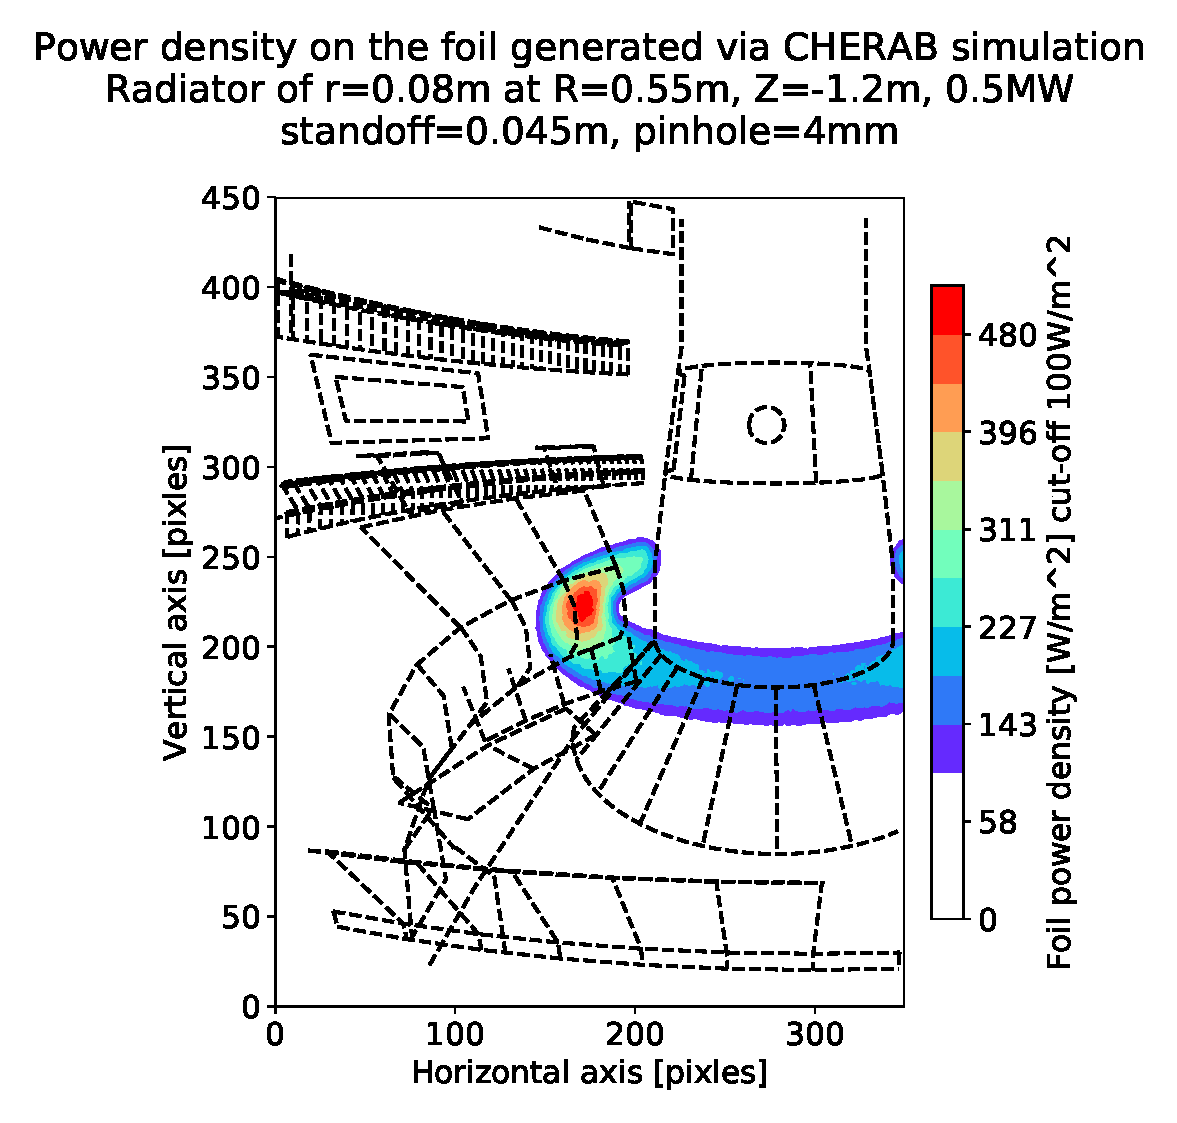
\includegraphics[trim={85 25 57 80},clip,width=\textwidth]{Chapters/chapter2/figs/measured_power_4_45radiator_R0.55_Z-1.2_r0.08.stl.eps}
         \caption{pinhole 4mm/stand-off 45mm}
         \label{fig:4_45}
     \end{subfigure}
     \hfill
     \begin{subfigure}{0.31\textwidth}
         \centering
         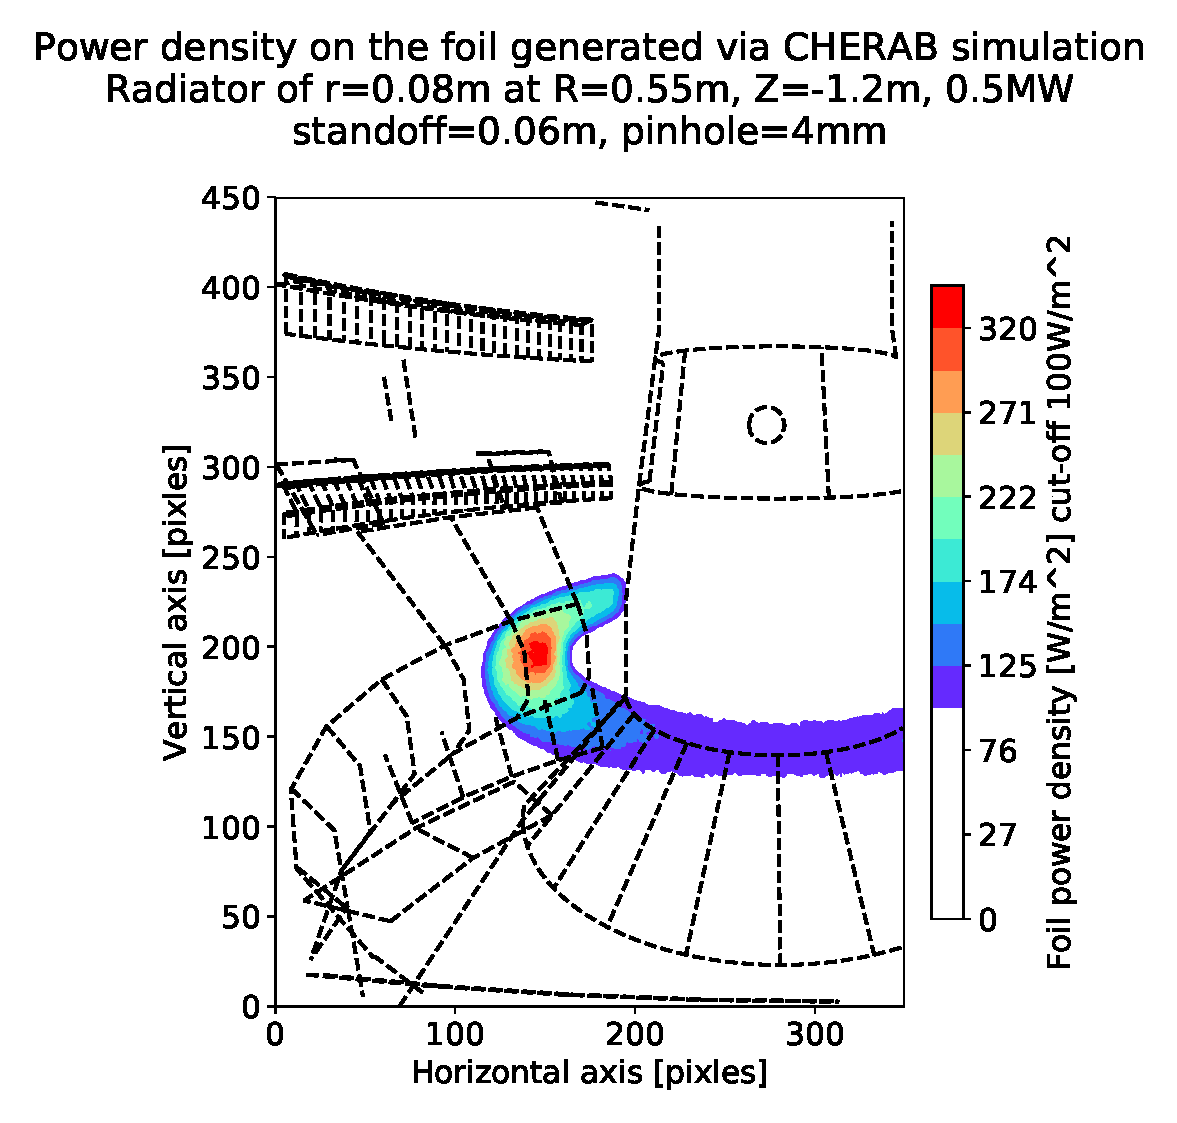
\includegraphics[trim={85 25 57 80},clip,width=\textwidth]{Chapters/chapter2/figs/measured_power_4_60radiator_R0.55_Z-1.2_r0.08.stl.eps}
         \caption{$4/60$}
         \label{fig:4_60}
     \end{subfigure}
     \hfill
     \begin{subfigure}{0.325\textwidth}
         \centering
         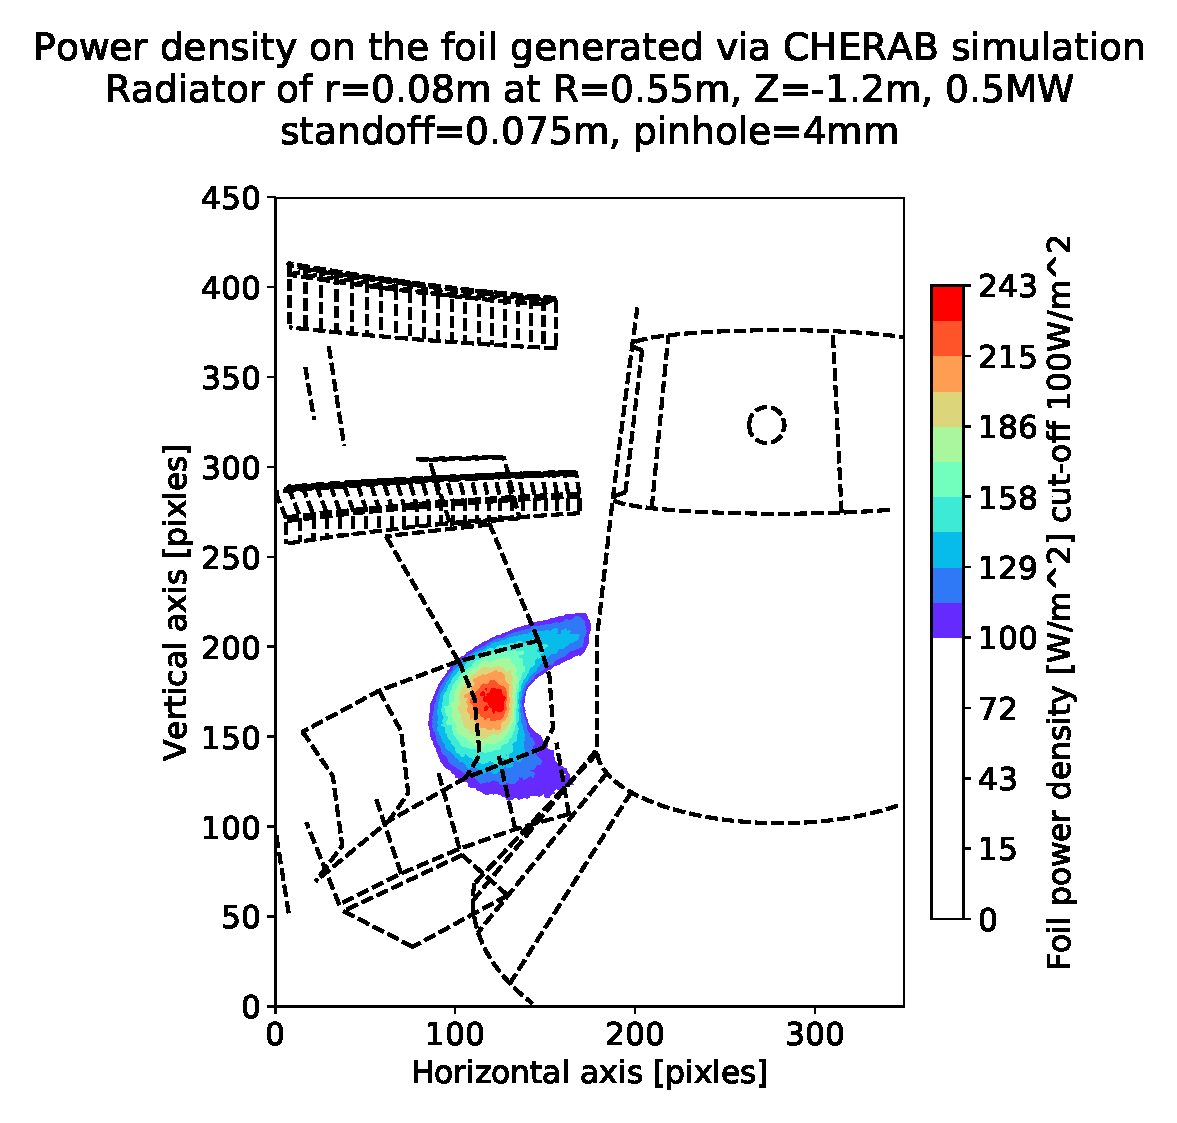
\includegraphics[trim={85 25 40 80},clip,width=\textwidth]{Chapters/chapter2/figs/measured_power_4_75radiator_R0.55_Z-1.2_r0.08.stl.eps}
         \caption{$4/75$}
         \label{fig:$4_75$}
     \end{subfigure}
     \begin{subfigure}{0.32\textwidth}
         \centering
         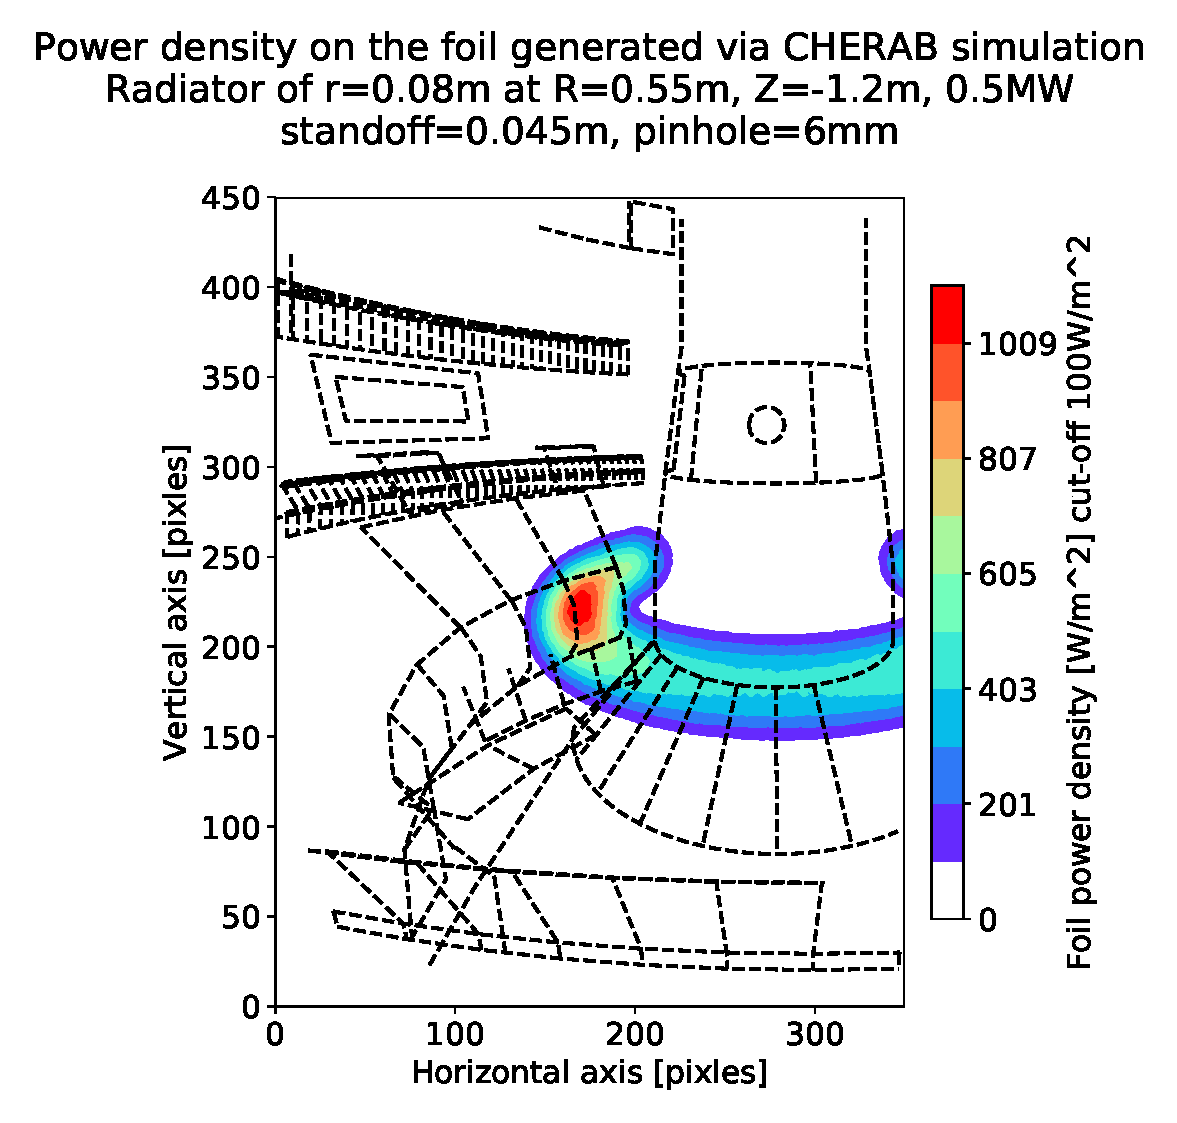
\includegraphics[trim={85 25 49 80},clip,width=\textwidth]{Chapters/chapter2/figs/measured_power_6_45radiator_R0.55_Z-1.2_r0.08.stl.eps}
         \caption{$6/45$}
         \label{fig:6_45}
     \end{subfigure}
     \hfill
     \begin{subfigure}{0.31\textwidth}
         \centering
         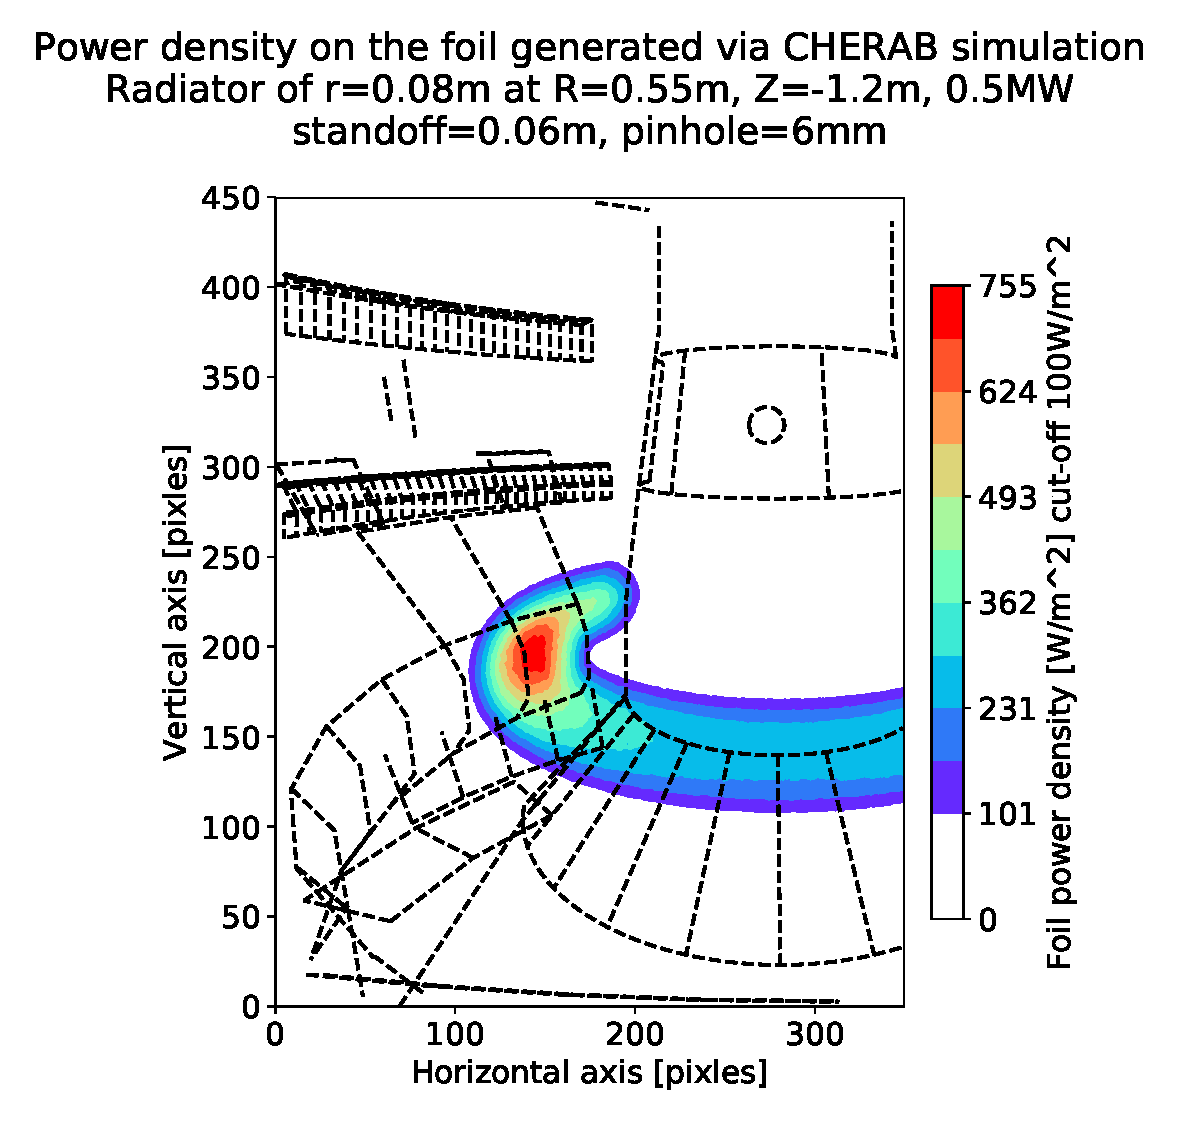
\includegraphics[trim={85 25 57 80},clip,width=\textwidth]{Chapters/chapter2/figs/measured_power_6_60radiator_R0.55_Z-1.2_r0.08.stl.eps}
         \caption{$6/60$}
         \label{fig:6_60}
     \end{subfigure}
     \hfill
     \begin{subfigure}{0.325\textwidth}
         \centering
         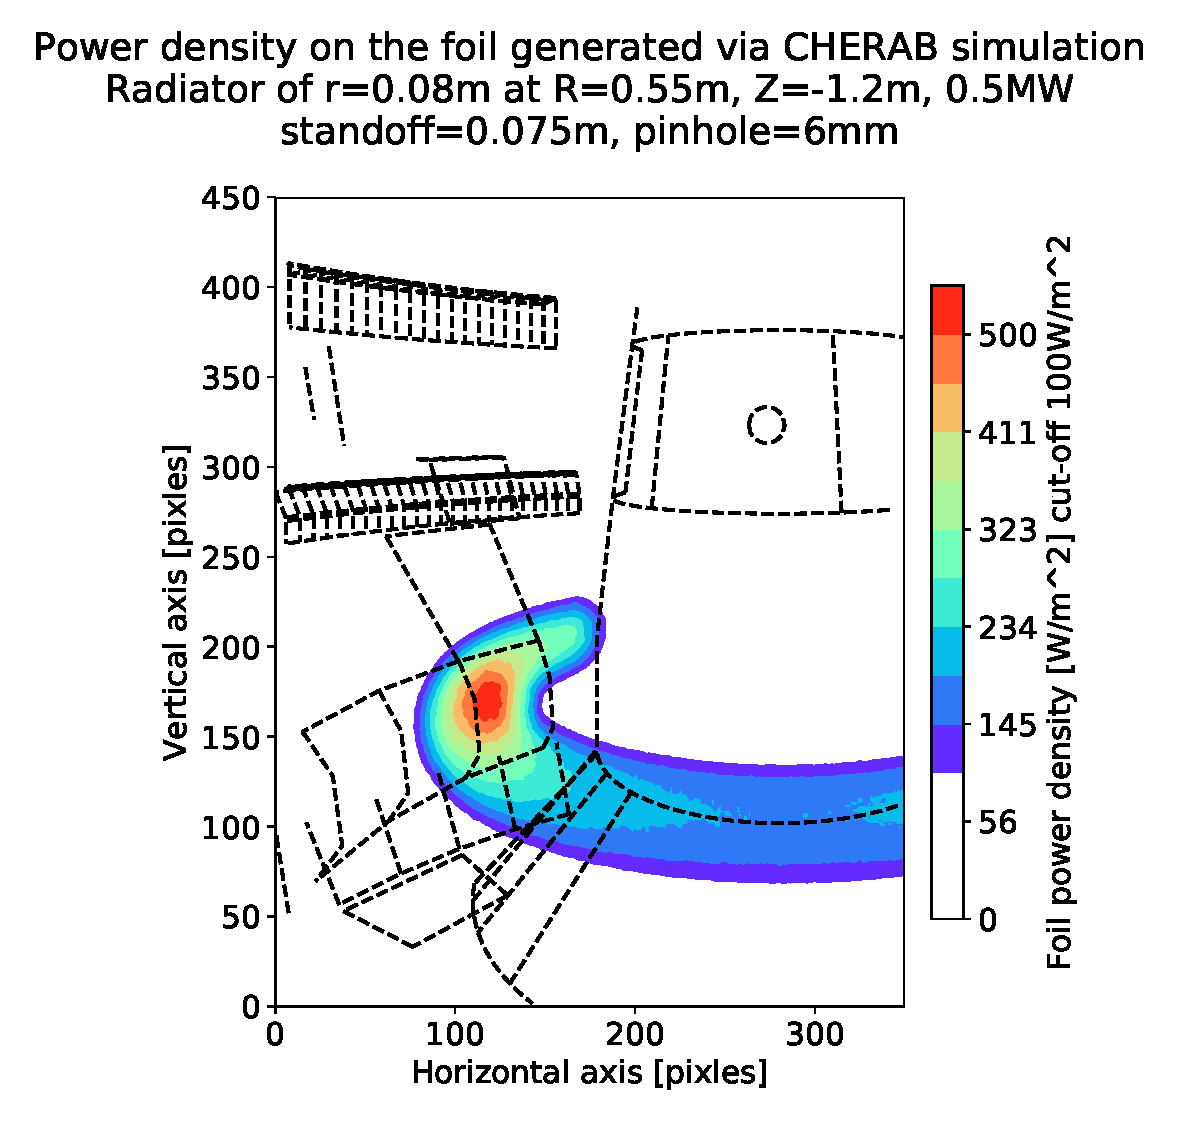
\includegraphics[trim={85 25 40 80},clip,width=\textwidth]{Chapters/chapter2/figs/measured_power_6_75radiator_R0.55_Z-1.2_r0.08.stl.eps}
         \caption{$6/75$}
         \label{fig:6_75}
     \end{subfigure}
     \begin{subfigure}{0.32\textwidth}
         \centering
         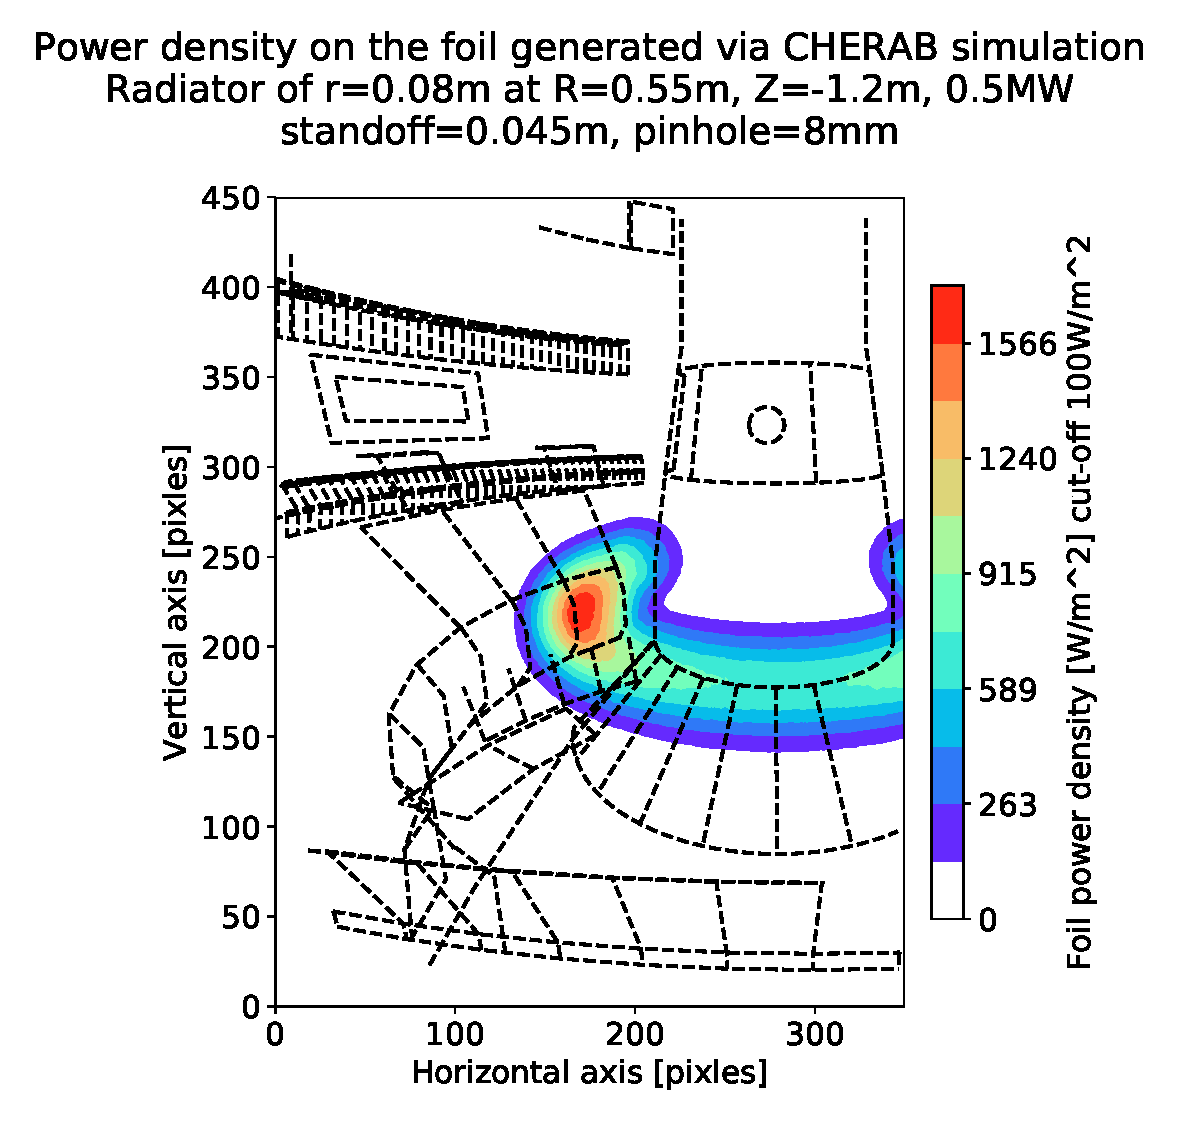
\includegraphics[trim={85 25 49 80},clip,width=\textwidth]{Chapters/chapter2/figs/measured_power_8_45radiator_R0.55_Z-1.2_r0.08.stl.eps}
         \caption{$8/45$}
         \label{fig:8_45}
     \end{subfigure}
     \hfill
     \begin{subfigure}{0.32\textwidth}
         \centering
         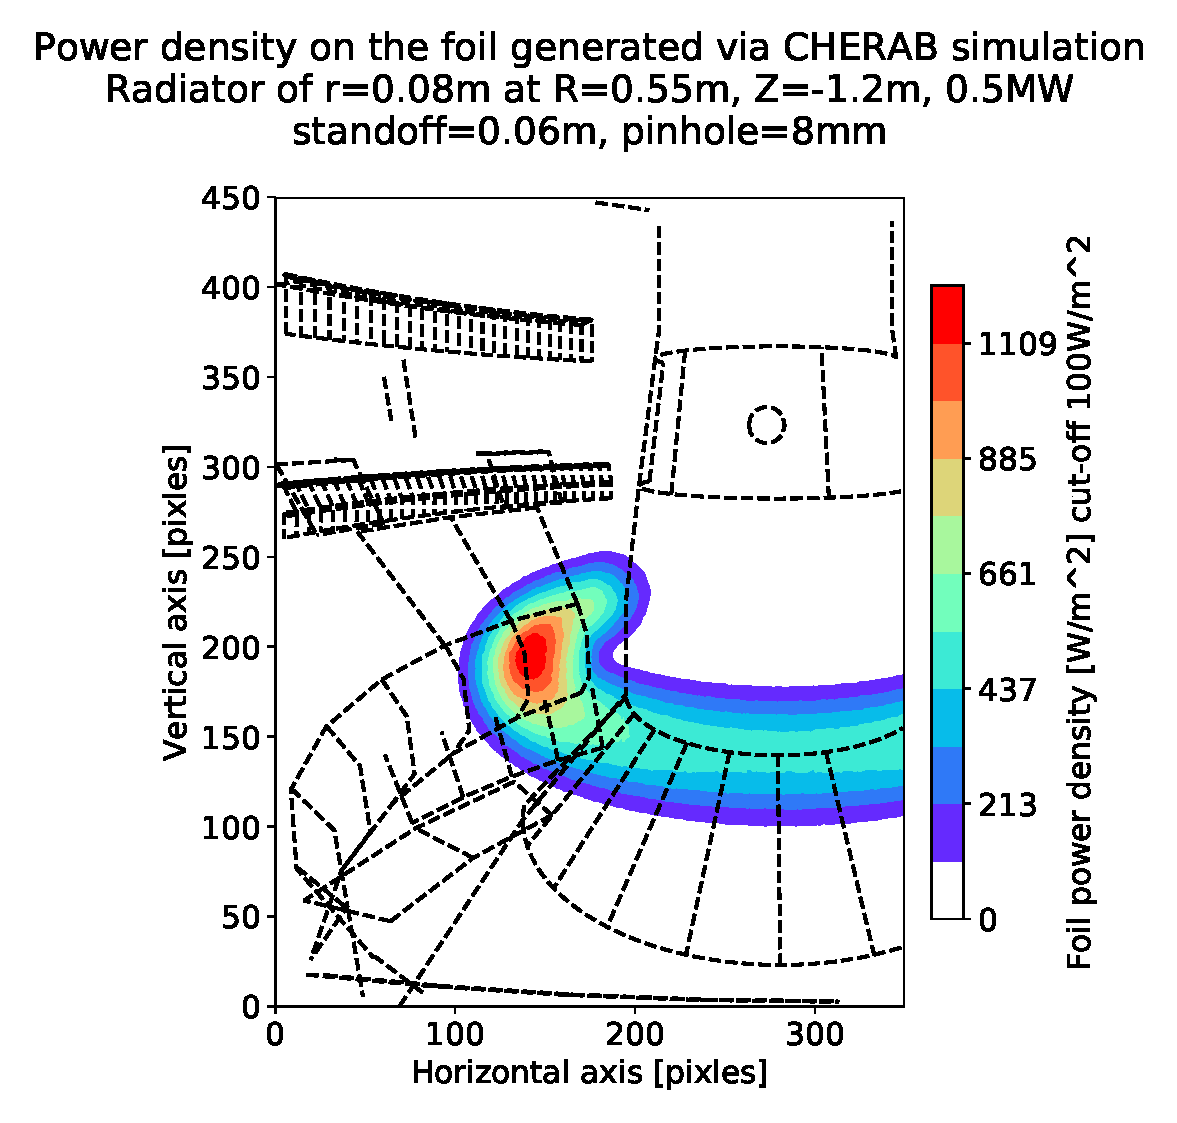
\includegraphics[trim={85 25 49 80},clip,width=\textwidth]{Chapters/chapter2/figs/measured_power_8_60radiator_R0.55_Z-1.2_r0.08.stl.eps}
         \caption{$8/60$}
         \label{fig:8_60}
     \end{subfigure}
     \hfill
     \begin{subfigure}{0.325\textwidth}
         \centering
         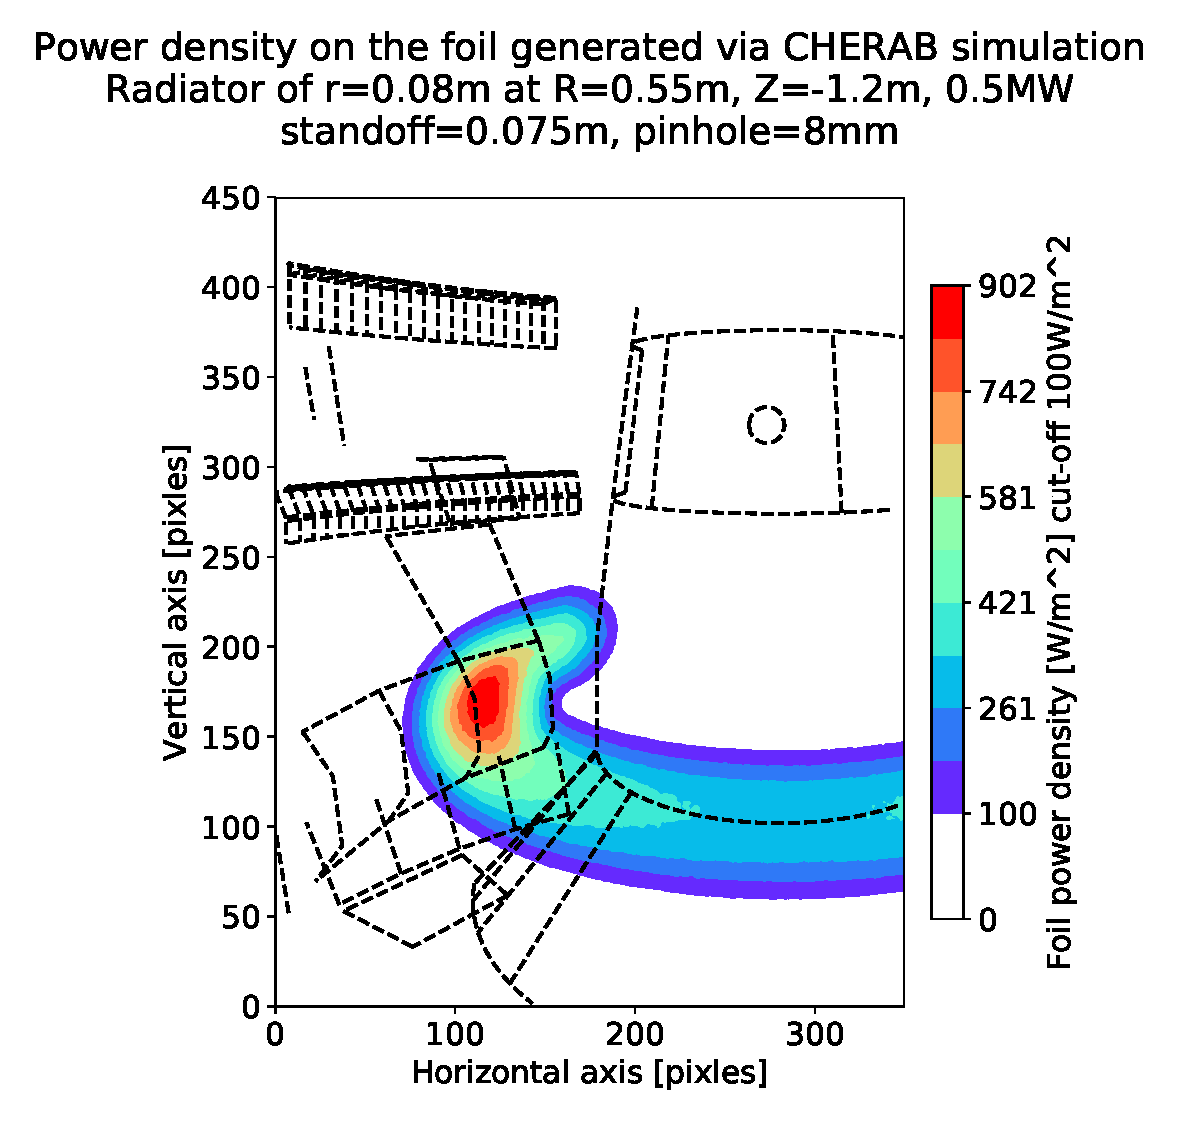
\includegraphics[trim={85 25 40 80},clip,width=\textwidth]{Chapters/chapter2/figs/measured_power_8_75radiator_R0.55_Z-1.2_r0.08.stl.eps}
         \caption{$8/75$}
         \label{fig:8_75}
     \end{subfigure}

    \caption{Radiated power deposited on foil from a homogeneous toroidal emitter of radius 8cm located at R=0.55m and Z=-1.2m, emitting a total of 0,5MW for the combinations of pinhole diameter and stand-off length considered. The power deposited on the foil below $100W/m^2$ is not shown, as that is the minimum desired signal level. In black are overlaid the projection of relevant features of MAST-U structure on the foil for reference.}
    \label{fig:cherab1}
\end{figure}

The power distribution on the foil was also simulated in the case of a core and divertor region filled with a homogeneous emitter.\cite{Federici2022} See \autoref{fig:cherab2}.

\begin{figure}
     \centering
     \begin{subfigure}{0.48\linewidth}
         \centering
         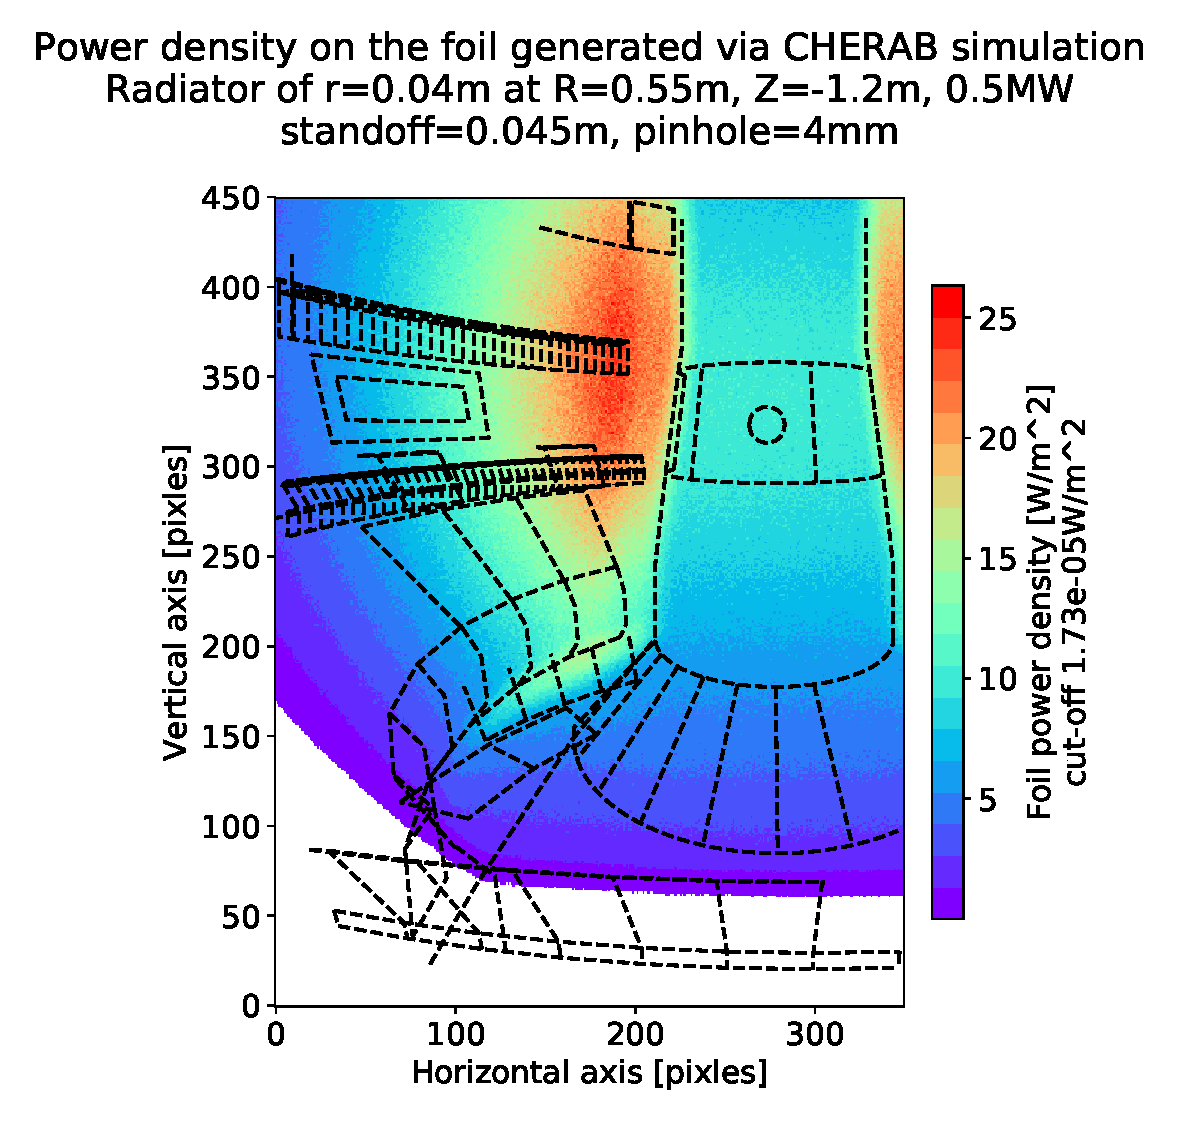
\includegraphics[trim={85 25 50 80},clip,width=\textwidth]{Chapters/chapter2/figs/measured_power_4_45radiator_all_core_and_divertor.stl.eps}
         \caption{pinhole 6mm/stand-off 45mm}
         \label{fig:4_45_all}
     \end{subfigure}
     \hfill
     \begin{subfigure}{0.48\linewidth}
         \centering
         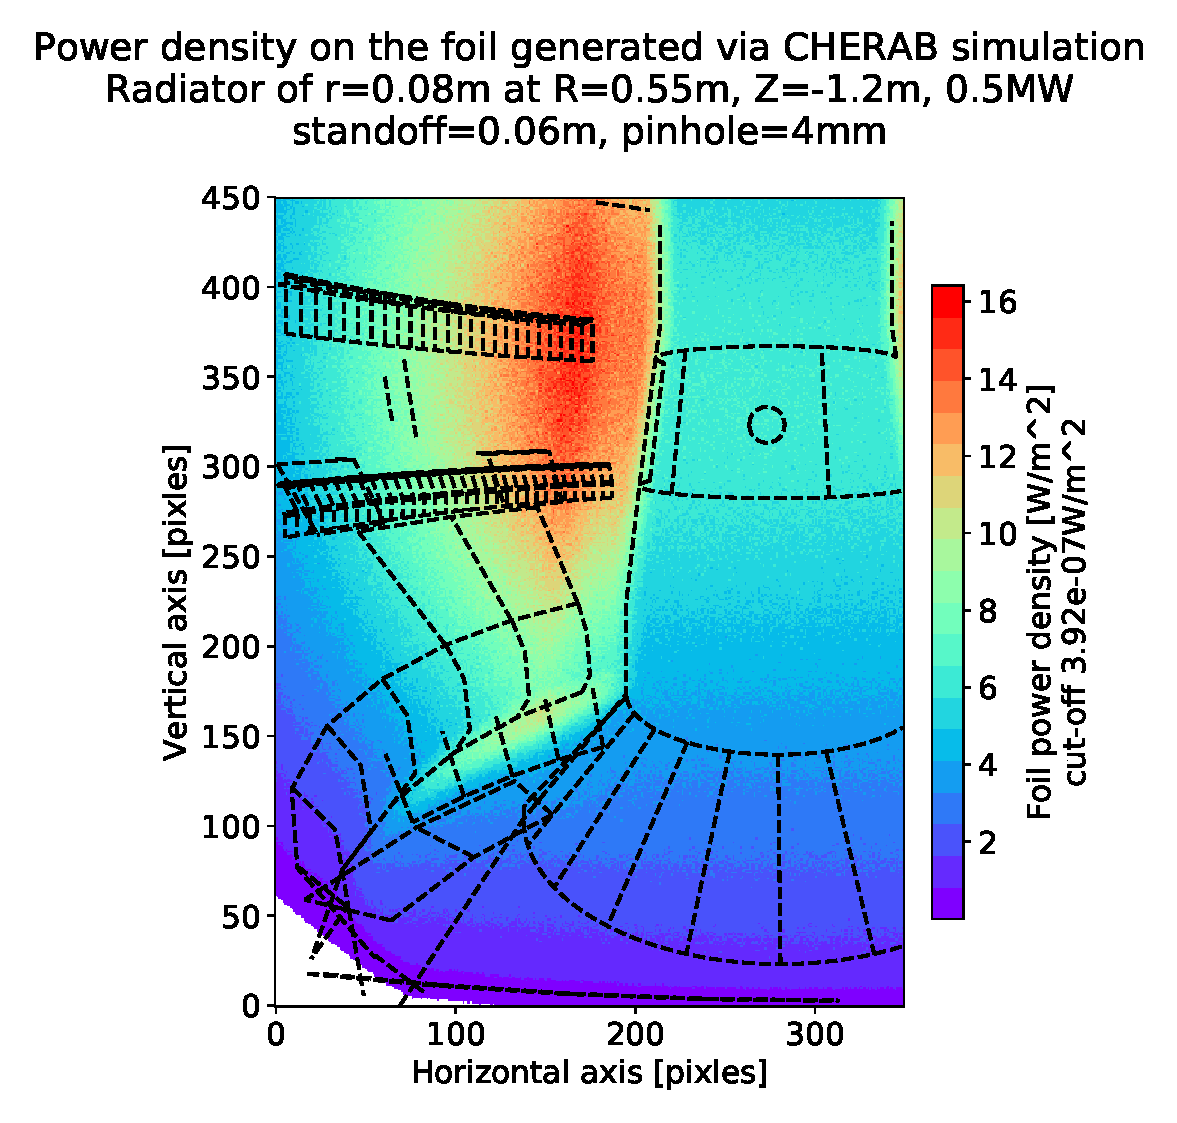
\includegraphics[trim={85 25 50 80},clip,width=\textwidth]{Chapters/chapter2/figs/measured_power_4_60radiator_all_core_and_divertor.stl.eps}
         \caption{$6/60$}
         \label{fig:4_60_all}
     \end{subfigure}

     \caption{Radiated power deposited on foil with a 4mm diameter pinhole and (\subref{fig:4_45_all}) 45mm and (\subref{fig:4_60_all}) stand-off between pinhole and foil, for the case of the core and divertor regions emitting homogeneously at a level of $50kW/m^3$. The white regions do not receive any radiation from the plasma, in black are overlaid the projection of relevant features of MAST-U structure on the foil for reference.}
    \label{fig:cherab2}
\end{figure}

\begin{figure}
     \centering
     \begin{subfigure}{0.7\linewidth}
         \centering
         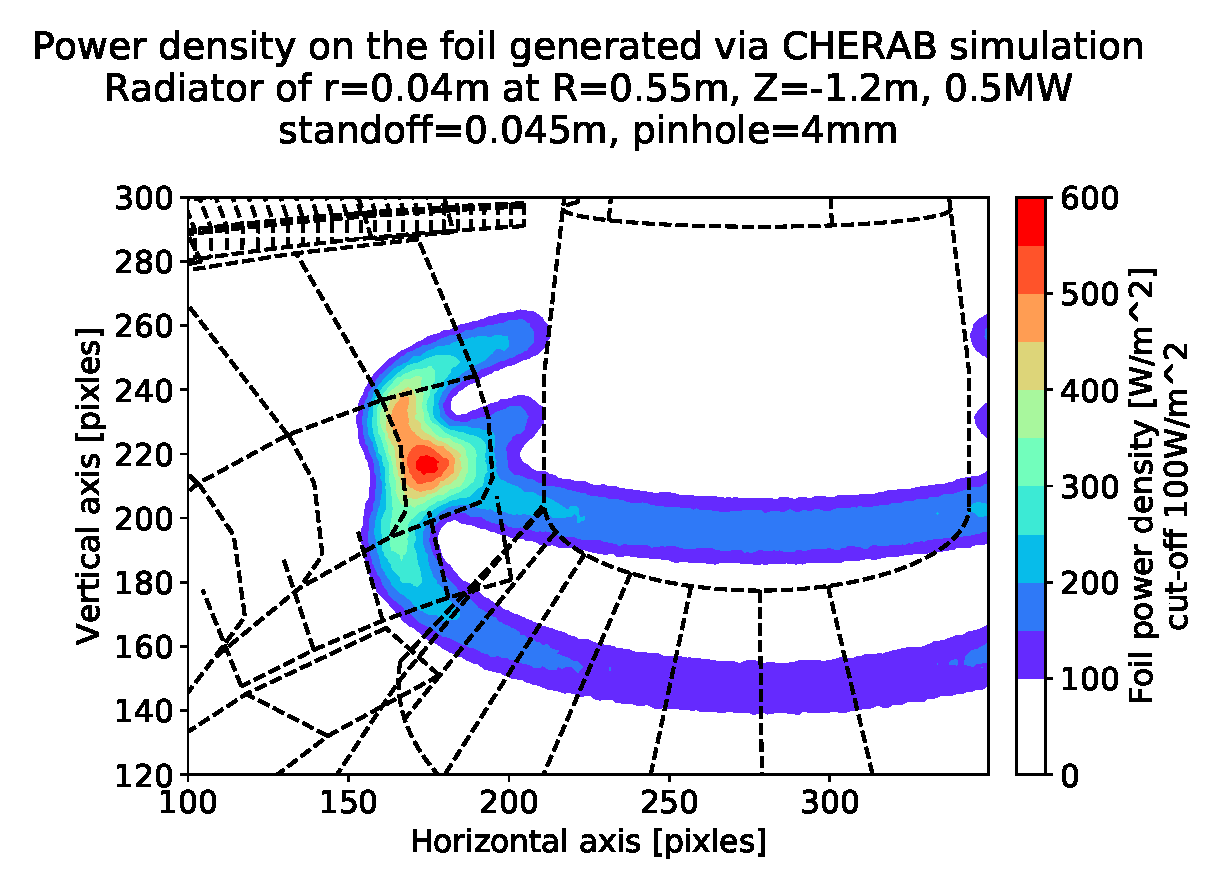
\includegraphics[trim={45 22 0 80},clip,width=\textwidth]{Chapters/chapter2/figs/measured_power_4_452x_radiator_R0.55_Z-1.2-1.3_r0.04.stl.eps}
         \caption{}
         \label{fig:pinhole_resolution4}
     \end{subfigure}
     \begin{subfigure}{0.7\linewidth}
         \centering
         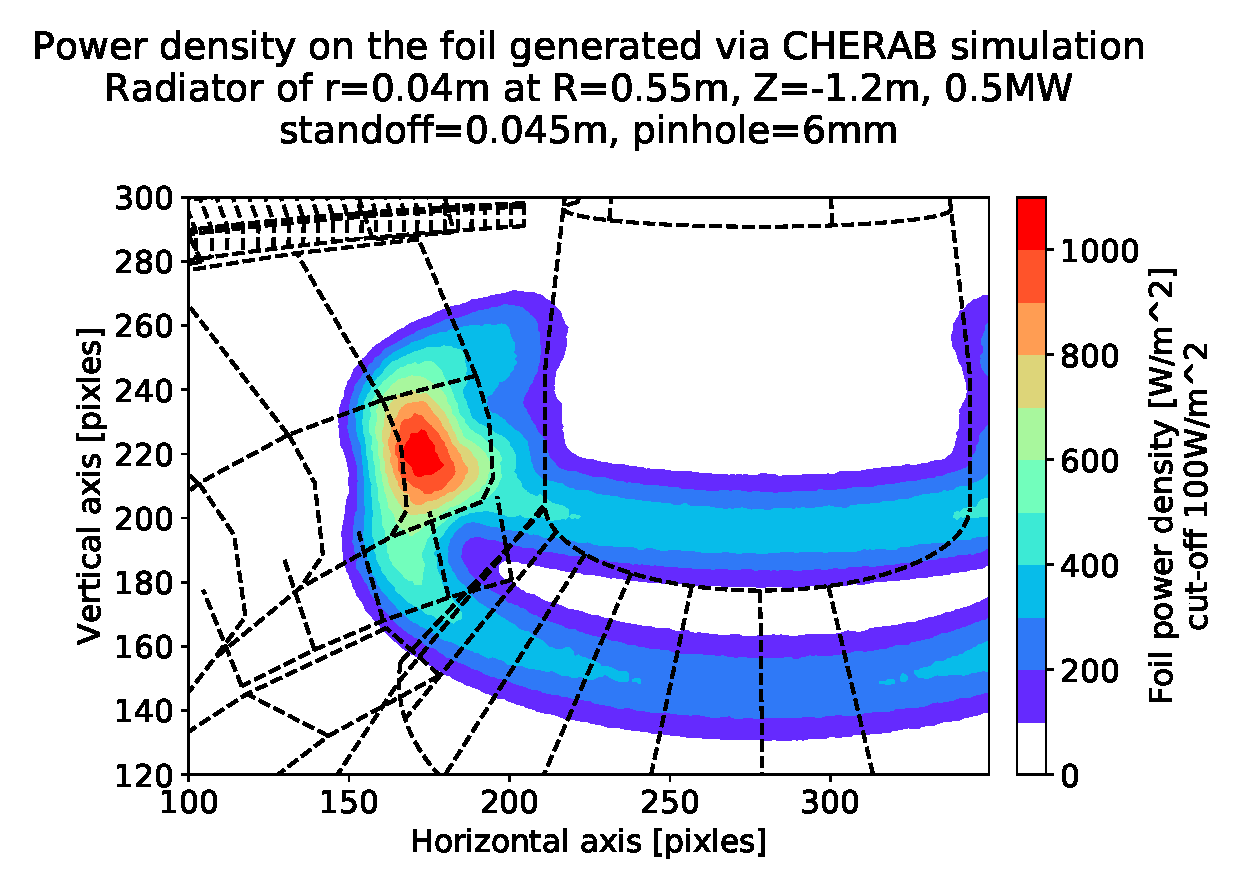
\includegraphics[trim={45 22 0 80},clip,width=\textwidth]{Chapters/chapter2/figs/measured_power_6_452x_radiator_R0.55_Z-1.2-1.3_r0.04.stl.eps}
         \caption{}
         \label{fig:pinhole_resolution6}
     \end{subfigure}
	\caption{Radiated power deposited on foil, modeled with CHERAB, of two toruses of 4 cm minor radius separated by 16cm in vertical position with uniform emissivity such as to total 0.5MW of radiated power, located at the expected x-point location. The pinhole size was varied from 4mm (\subref{fig:pinhole_resolution4}) to 6mm (\subref{fig:pinhole_resolution6}) to illustrate the loss of spatial resolution. The power deposited on the foil below $100W/m^2$ is not shown, as that is the minimum desired signal level. Only the relevant section of the foil is shown. In black are overlaid the projection of relevant features of MAST-U structure on the foil for reference.}
    \label{fig:pinhole_resolution}
\end{figure}


The bottom left region of the image is where no radiation can arrive. This could have been helpful for the prototype phase, because that area could have been used as a reference where the power is zero.
For this reason it has been decided to adopt a stand-off between pinhole and foil distance of 45mm for MU01, which covers results shown in this thesis. This allows for an intense enough radiation from the X-point to adopt a relatively small 4mm diameter pinhole, allowing for better resolution. In \autoref{fig:pinhole_resolution} it is illustrated how, with a smaller pinhole, the signal level is lower but it is easier to identify close but distinct structures in the radiation distribution, even from the poloidal view alone (left side of the foil). For closer toruses it would be easier to distinguish them as separate in the tangential view (right side of the foil) with a smaller rather than large pinhole. The MAST-U IRVB diagnostic has been returned to operation on MAST-U for the second campaign (MU02) with a stand-off of $60mm$, which enables higher spatial resolution within the divertor region, after re-evaluating the nose levels (see \autoref{MU02 geometry optimisation}).

An approximate view inside MAST-U, imagining that the IRVB operates as a camera to show the features and obstructions, is shown in \autoref{fig:calcam}. The view of the plasma is mainly poloidal on the left side of the central column, but the field of view is large enough to see both sides of the central column.

\begin{figure}
	\centering
	\includegraphics[trim={30 30 450 90},clip,width=0.5\linewidth]{Chapters/chapter2/figs/calcam4.png}
	\caption{Approximate view inside MAST-U as if the IRVB operates as a camera. Blue labelling is used to highlight the various sectors and the fuelling locations in the IRVB field of view (FOV). At the bottom of the image is the coil P6 obstructing the field of view.}
	\label{fig:calcam}
\end{figure}

\begin{figure}
     \centering
     \begin{subfigure}{0.48\linewidth}
         \centering
         \includegraphics[trim={175 20 65 60},clip,width=\textwidth]{Chapters/chapter2/figs/res_bolo5.png}
         \caption{}
         \label{fig:res_bolo1a}
     \end{subfigure}
     \begin{subfigure}{0.48\linewidth}
         \centering
         \includegraphics[trim={20 0 70 0},clip,width=\textwidth]{Chapters/chapter2/figs/res_bolo_toroidal3.png}
         \caption{}
         \label{fig:res_bolo1b}
     \end{subfigure}
	\caption{(\subref{fig:res_bolo1a}) Poloidal view of MAST-U showing the comparison of the resistive bolometer system LOS (magenta) with a color plot obtained by scanning all the voxels with a $1W/m^3$ emitter and integrating the power absorbed by the foil, indicating the regions of higher sensitivity of the IRVB. (\subref{fig:res_bolo1b}) Top view of MAST-U showing the position of neutral beam injectors (NBI, green), of the co- and counter-NBI resistive bolometer LOSs and the IRVB FOV (yellow, mostly counter-NBI). Adapted from \cite{Rivero-Rodriguez2018}. For reference the separatrix of a typical plasma is shown as an overlay of a blue dashed line. The resistive bolometer LOSs that will be used in the later analysis are here identified. The LOSs not operational in MU01 are red rather than magenta. The location of CH9 in \subref{fig:res_bolo1b} indicates where the entire core tangential fan is located.}
    \label{fig:res_bolo1}
\end{figure}


\autoref{fig:res_bolo1} displays the overlap between the coverage and views of the resistive bolometry system and that of the IRVB. The core resistive bolometer LOSs are mostly suited to measure the fairly homogeneous core emissivity profiles on a flux surface, as there is no overlap between the various LOS. The super-x chamber has a good coverage, but only between the  strike point and the entrance to the divertor defined by the baffle. The IRVB is aimed to fill the gap between the two systems.

The assembly holding the foil is composed by a $2.5\mu m$ thick platinum foil from Nilaco, Japan, held between oxygen free copper plates and was originally prepared by NIFS. The foil is the same as that used in Alcator C-mod\cite{Reinke2018a} where it is described in more detail. The foil thickness is optimised to stop photons with energies up to $8.2keV$. \cite{PETERSON2010,Gullikson2022} The foil and its support frame have been spray blackened on both sides with Aerodag® G Graphite Aerosol and calibrated with a procedure analogous to the one described in \cite{Itomi2014}. The layer of graphite helps to absorb radiation in the visible range, avoiding reflection; even if its thickness is larger than the platinum layer\cite{Pandya2014} it should be thermally irrelevant. \cite{VanEden2018} Lower energy photons like visible light represent a minor energy loss channel, but their relevance is expected to increase in deeply detached and cold plasmas, therefore the importance of the coating.\cite{Havlickova2015a} In \cite{Mukai2016} it is shown that this type of coating causes irregularities in the foil, leading to non uniform temperature increases. To alleviate this issue, the carbon layer can be deposited with a vacuum evaporation technique that guarantees reproducibility and uniformity, as done at LHD. \cite{Mukai2016} Given the prototype nature of the present implementation and the availability of a vacuum compatible certified absorber, this foil was deemed sufficient.

\begin{figure}
     \centering
     \begin{subfigure}{0.35\linewidth}
         \centering
         \includegraphics[trim={0 0 600 0},clip,width=\textwidth]{Chapters/chapter2/figs/foil_markings3.png}
        %  \caption{386ms}
         \label{fig:foil markings1}
     \end{subfigure}
     \begin{subfigure}{0.63
     \linewidth}
         \centering
         \includegraphics[trim={50 0 0 0},clip,width=\textwidth]{Chapters/chapter2/figs/foil_markings.png}
        %  \caption{511ms}
         \label{fig:foil markings2}
     \end{subfigure}
    \caption{Photographs of the foil in relation of the pinhole (a) and of all the identifying markings (b), taken 23/07/2018.}
    \label{fig:foil markings}
\end{figure}

To guarantee consistency in the positioning and orientation of the foil with respect to the pinhole, a series of markings were inscribed by NIFS on the copper plates as shown in \autoref{fig:foil markings}. The yellow numerical markings are also used to define the thermal calibration supplied with the foil.
The compatibility of the assembly with the thermal expansion caused by the MAST-U VV bake was studied. The bake causes the VV and internal components to reach $\sim110\degree C$ and 120 to $200\degree C$ respectively, likely causing the absorber assembly to reach an intermediate temperature. The thermal expansion coefficients for Cu and Pt are $16 \mu m/mK$ (similar to steel) and $9 \mu m/mK$ respectively. This could have led to stress and thus tearing of the foil, but confidence was gained with the pressure test mentioned in \autoref{MAST-U IRVB design} on the mechanical resilience of the foil. Another item of concern related to the bake is the stability of the carbon coating on the absorber foil. The technical datasheet for Aerodag® G used for coating, indicates that it can be used as lubricant up to $200 \degree C$. Considering the possible failure modes, any piece of carbon detaching from the absorber assembly was expected to stay within the tube, posing no risk for MAST-U operations. The IRVB has ultimately undergone the entire bake cycle prior to MU01 and after inspection did not seem to suffer any damage.

The tube where the foil is installed extends from the vacuum chamber wall to a position close to the plasma, but still safely outside the SOL and potential particle and power loads. The camera images the absorber foil through a $10mm$ thick ZnS view port from Crystran with $4-5 \mu m$ and $8-10 \mu m$ anti reflection coating on both sides and is bolted to the tube. The orientation of the view port with respect to the camera, even if it should not matter substantially, was maintained throughout the test and assembly phases for consistency. The view port assembly was leak checked before final installation with the setup in \autoref{fig:vacuum_setup}. 
The camera, a FLIR SC7500 with InSb detector array, is equipped with a $4-5\mu m$ pass band filter and has a spectral range of $1.5-5.1\mu m$. This model was selected so that the same could be adopted for other diagnostics in MAST-U and the same acquisition software could potentially be developed. This is inconvenient for the IRVB, as the optimal wavelength for a black body radiator around room temperature is around $10-14\mu m$. Considering that the volume between foil and camera is fully enclosed in the IRVB tube and that the temperature of the entire assembly does not deviate appreciably from room temperature during the short duration of the pulse, the use of the filter would not have prevented any stray light to effect the measurements. For this reason the camera was used without the internal filter, increasing the signal. At the maximum frame rate at full frame (383Hz) and 2ms integration time a strong signal around 11000 counts is measured (see \autoref{fig:example_BB_fit}) with saturation at $2^{14}=16384$ counts and a noise floor $\sim5$ counts.
During testing a design flaw of the present IRVB design was discovered. It became clear that, even with the presence of the anti reflection coating, the view port caused the so-called "narcissus effect". This happens when the camera can see its own reflection on the view port, hence "narcissus". The view is orthogonal to the camera FOV, so at its center is the image of the reflection of the sensor array. The detector array is cooled to about $-203\degree C$, while around it the body of the camera is slightly above room temperature. This causes a "dark spot" to appear at the centre of the image. The main difficulty in dealing with the effect arises from the inability to perfectly match the orientation of the view port during calibration and on the machine. Ultimately this systematic error, if stable intra-shot, does not effect the temporal and spatial temperature derivatives on which the analysis primarily relies. In future iterations of the diagnostic, the view port should be angled with respect to the camera so as to reflect light from an area with a more homogeneous temperature and emissivity.

The camera is bolted to aluminum plates cantilevered off an insulating G-10 piece that is connected directly to the vacuum vessel flange (to stop induced current loops) as shown in \autoref{fig:IRVB_components}. The aluminum plates holding the camera have multiple holes so that the camera can be located at 4 fixed distances from the the view port (8.7, 11.2, 13.7, $16.2cm$), with the closest being the one with the foil in focus. The ability to vary the camera location allowed us to progressively test the compatibility of the camera with magnetic field. That data was collected during the commissioning phase of the MAST-U magnets while the camera was first as far as possible from the VV. Once the maximum field was reached the camera was then progressively moved towards its final position whilst checking that no anomalies in its operation arose. The camera operated normally at all distances, making a magnetic shield around it unnecessary.

The IRVB tube was installed on MAST-U in November 2018 while all parts outside the vacuum vessel by early 2021. The calibration of the system was performed in 2018.


\section{System calibration}\label{System calibration}
Before scientific utilization, the IRVB diagnostic has to be properly calibrated. This includes the temperature response of the IR camera, the thermal response of the foil and spatial alignment of the pinhole and camera. Laboratory tests can be performed for the first two calibrations, while the third was verified during operation, using observed features inside the tokamak.

% old sections where the method uses the black body source as close as possible to the window
% \subsection{Counts to temperature model}\label{Counts to temperature model}
% The temperature calibration is the procedure used to convert the camera row data from counts to temperature. It involves defining the mathematical model for the conversion and finding the coefficients required. Once defined it can be applied to MAST-U data to obtain the IRVB foil temperature.
% The surface of the foil is approximated as a black body emitter. The photons emitted by a BB source within the camera integration time can be modelled as \autoref{eq:BBphotons1}


% \begin{equation}
% {\Phi}_p (T) = \epsilon i \int_{ {\lambda}_1 }^{ {\lambda}_2 } {\frac{2 \pi c } { {\lambda}^4 } \frac {1} { e^{\frac {hc} {\lambda k T}} -1} {d \lambda} }
% \label{eq:BBphotons1}
% \end{equation}

% with $\epsilon$ emissivity, $i$ integration time, $\lambda$ wavelength and $\lambda_1-\lambda_2$ the range allowed by the camera filter and $T$ the surface temperature.
% To simplify the calculations an interpolator is built such that

% \begin{equation}
% \frac {{\Phi}_p (T)} {T} = \alpha (T) , T = {\alpha}_r ({\Phi}_p)
% \label{eq:BBphotons2}
% \end{equation}

% The number of photons reaching the camera are going to be proportional to the number of emitted photon ($a_1$), with an additional offset due to thermal photons originated from other solid surfaces and the air ($a_2$). This offset will be approximately constant because it will not depend on the surface temperature observed by the camera.
% The presence of the view port between camera and the source of BB radiation will decrease the number of thermal photons reaching the camera ($a_3$) and potentially modifies the constant offset ($a_4$).
% Assuming that the number of counts is proportional to the number of photons, and that this does not depends on the photon wavelength, the number of camera counts can be expressed as:

% \begin{equation}
% C = a_1 \cdot a_3 \cdot {\Phi}_p (T) + a_2 + a_4
% \label{eq:BBphotons3}
% \end{equation}

% with $a_1\in[0,\infty]$ and $a_2\in[-\infty,\infty]$ the proportional and constant component for the counts without the view port and $a_3\in[0,1]$ and $a_4\in[-\infty,\infty]$ the modifiers for the view port case. $T_0$ and $C_0$ are the temperature and counts relative to the initial conditions at the beginning of the shot (room temperature).
% In order to calculate all 4 coefficients 2 temperature ramps are required, one with and one without view port. When changing the temperature of the BB source the camera counts have to be monitored to make sure to collect the data only after they have stabilised.
% The counts/temperature curves obtained are then fit to return the coefficients. The power absorbed by the IRVB foil is obtained using the temperature increase over the profile before the pulse ($T_0$ and $C_0$), so the constant offset from the calibration will not impact the results while its uncertainty will impart the result uncertainty, even if usually negligibly.
% Once $a_1 \cdot a_3$ is determined the temperature is calculated as:

% \begin{equation}
% T = {\alpha}_r ( {\Phi}_p(T)) = {\alpha}_r \left (\frac {C - a_2 - a_4} {a_1 \cdot a_3} \right ) = {\alpha}_r \left (\frac {C - C_0} {a_1 \cdot a_3} + {\Phi}_p (T_0) \right )
% \label{eq:BBphotons4}
% \end{equation}


% \subsection{Temperature calibration}


% In order to test every pixel of the camera with the limited size of the BB source available the source was taken as close as possible to the view port making it out of focus. This could be done as the whole surface of the BB cavity emits the same amount of radiation isotropically. For the pixels whose entire field of view is inside the source from when it is in focus to when it's closer the etendue is conserved, allowing to perform the calibration. A series of measurements was performed to verify this by changing the distance between the camera and the black body source at room temperature and with a hot black body source. The black body source employed was a MIKRON M315HT with a range of ambient temperature $+10\degree C/+450\degree C$ therefore to calibrate the camera in the useful temperature of ambient $+0\degree C/+10\degree C$ the ambient temperature was lowered to about $5\degree C$. The infrared camera is equipped with 2 distinct digitizers therefore the calibration will be operated independently for each. This means that formally the two digitizers behave as 2 distinct instruments; the power absorbed by the foil will be calculated independently for each and then averaged, causing a reduction of the maximum frame rate from 383Hz to 192Hz.

% \hl{example of vignetting and narcissus}

% \begin{figure}
% 	\centering
% 	\includegraphics[trim={40 5 70 50},clip,width=\linewidth]{Chapters/chapter2/figs/counts vs distance2.png}
% 	\caption{Average counts for pixels that always image the inside of the black body source. The viewport was not present for this measurements. The error bar represent the variation of the reading within the region.}
% 	\label{fig:counts vs distance2}
% \end{figure}
% In \autoref{fig:counts vs distance2} is shown the variation with distance of the average counts for pixels that always image the black body source. The variation is small but not negligible (400 counts correspond to about $1\degree C$ variation). The cause of the variation cannot be identified but could be reflections or the effect of line absorption in the observed wavelength window ($2.5-5 \mu m$, $CO_2$ has a line at $\sim 4.2 \mu m$). The configuration that is closer to the experimental conditions is the one with the black body source as close as possible to the view port as vacuum is present inside the vessel so this will be used.

% \begin{figure*}
% 	\centering
% 	\includegraphics[trim={750 300 0 1200},clip,width=\linewidth]{Chapters/chapter2/figs/calib_schematics.png}
% 	\caption{Schematic of the calibration setup. The plane in focus correspond to the distance at which the IRVB foil is. The view port is at the same distance from the camera as when installed on MAST-U. The location used to measure the distance of the camera from other objects is marked in red.}
% 	\label{fig:BBcalib}
% \end{figure*}

% The geometry of the calibration is represented in \autoref{fig:BBcalib}. As it takes time for the black body source temperature to stabilise the view port is installed in such a way that it can reliably removed and placed back with the same orientation. This allows to do both temperature scans with and without view port in a single source temperature scan.

% \begin{figure}
%      \centering
%      \begin{subfigure}{\linewidth}
%          \centering
%          \includegraphics[trim={0 0 0 25},clip,width=\linewidth]{Chapters/chapter2/figs/example_BB_fit(0, 128, 50).png}
%          \caption{digitizer 0, pixel (128,50)}
%          \label{fig:example_BB_fit(0, 128, 50)}
%      \end{subfigure}
%      \hfill
%      \begin{subfigure}{\linewidth}
%          \centering
%          \includegraphics[trim={0 0 0 25},clip,width=\linewidth]{Chapters/chapter2/figs/example_BB_fit(0, 128, 160).png}
%          \caption{digitizer 0, pixel (128,160)}
%          \label{fig:example_BB_fit(0, 128, 160)}
%      \end{subfigure}

%     \caption{Comparison of the temperature calibration curves for a pixel at the centre of the aberration (\subref{fig:example_BB_fit(0, 128, 160)}) with one on its side (\subref{fig:example_BB_fit(0, 128, 50)}). In yellow is indicated the fit of the data with \autoref{eq:BBphotons3} and in the legend the corresponding coefficients.}
%     \label{fig:example_BB_fit}
% \end{figure}

% The result of the scan for two pixels, one at the centre of the aberration caused by the view port and one on its side, are shown in \autoref{fig:example_BB_fit}. \autoref{eq:BBphotons3} can reproduce the measurements with high accuracy and the effect of the presence of the view port can be readily extracted. As expected, most of the flat offset is in $a_2$ while only a minor component in $a_4$.

% The results of the calibration for the entire foil are shown in \autoref{fig:BBcaliba1}, \ref{fig:BBcaliba3} and \ref{fig:BBcaliba1a3SNR}. The $a_1$ coefficient seems completely not effected by the narcissus effect. Conversely the corrective factor $a_3$ seems dominated by it, while still being $>0.95$ across the thole field of view with a relative variation less then half of $a_1$. The $a_2$ and $a_4$ coefficients are irrelevant as are not used in the temperature and power calculations.

% \begin{figure}
% 	\centering
% 	\includegraphics[trim={140 40 120 50},clip,width=\linewidth]{Chapters/chapter2/figs/calib_a1_2.png}
% 	\caption{$a_1$ coefficient obtained via calibration with BB source}
% 	\label{fig:BBcaliba1}
% \end{figure}
% \begin{figure}
% 	\centering
% 	\includegraphics[trim={140 40 120 50},clip,width=\linewidth]{Chapters/chapter2/figs/calib_a3_2.png}
% 	\caption{$a_3$ coefficient obtained via calibration with BB source}
% 	\label{fig:BBcaliba3}
% \end{figure}
% \begin{figure}
% 	\centering
% 	\includegraphics[trim={140 40 120 50},clip,width=\linewidth]{Chapters/chapter2/figs/calib_a1a3SNR_2.png}
% 	\caption{$a_1 a_3 / \sigma_{a_1 a_3}$ obtained via calibration with BB source}
% 	\label{fig:BBcaliba1a3SNR}
% \end{figure}

% To further verify the effect of the distance 3 separate calibrations were performed: camera and BB source as close as possible ($\sim 10cm$, some room was necessary for the view port in between the two), as far as possible (with the whole field of view still inside the source, $\sim 18cm$) and with the source in focus ($65.7cm$).

% \begin{figure}
% 	\centering
% 	\includegraphics[trim={0 0 40 30},clip,width=\linewidth]{Chapters/chapter2/figs/a1 vs distance.png}
% 	\caption{Variation with the source to camera distance of the average of the a1 coefficient over pixels that image the inside of the black body source. The viewport was not present for this measurements. The error bar represent the variation of the coefficient within the region.}
% 	\label{fig:a1 vs distance}
% \end{figure}
% The effect of the distance of the source on the a1 coefficient is shown in \autoref{fig:a1 vs distance} where the $a_1$ coefficient is averaged over the pixels that always image the inside of the source. The variation is approximatively 1.5\% that, considering small temperature differences in time or space, translate to an error of about 1.5\% in the temperature difference, negligible compared to other sources of error.

% An alternative method for temperature calibration was also tested. A Sofradir non uniformity calibration (NUC) plate, was pre-heated or cooled to a set temperature and let transition to room temperature. The NUC plate is large enough to fill the entire field of view and while in focus. Its surface is such to have an emissivity close to 1. The temperature of the plate is recorded and various samples are collected with the IR camera while the plate temperature approaches ambient. The data is then fit with a low order polynomial curve. This procedure introduces 2 issues:
% \begin{itemize}
%     \item the NUC plate is cooled or heated by the air via conduction, convection and BB radiation. This causes the plate to not have a homogeneous temperature. During these tests it was estimated that the temperature non uniformity reached $\sim$0.4K, and up to 0.1K in the -5/+5K temperature range around room temperature. This is of course not ideal for the IRVB, as the measurement of the power absorbed by the foil relies on very small temperature differences
%     \item The temperature/counts correlation does not rely on to a physical model, but it is a simple polynomial that will try to match the real physical dependency behind the IR measurements. The physics of a BB source is fairly simple, and the only factors are the wavelength range and emissivity. The camera could potentially have a different sensitivity for different photon energy, but this is usually neglected given the small wavelength range allowed by the filter ($2,5-5\mu m$).
% \end{itemize}
% For these reasons this method was later abandoned.


% new sections where the data is from the NUC plate but the fit is done with the BB model
\subsection{Counts to temperature model}\label{Counts to temperature model}
The temperature calibration is the procedure used to convert the camera raw data from counts to temperature. It involves defining the mathematical model for the conversion and finding the coefficients required. Once defined it can be applied to MAST-U data to obtain the IRVB foil temperature.
The surface of the foil is approximated as a black body emitter. The photons emitted by a BB source within the camera integration time can be modelled as \autoref{eq:BBphotons1}


\begin{equation}
{\Phi}_p (T) = \epsilon i \int_{ {\lambda}_1 }^{ {\lambda}_2 } {\frac{2 \pi c } { {\lambda}^4 } \frac {1} { e^{\frac {hc} {\lambda k T}} -1} {d \lambda} }
\label{eq:BBphotons1}
\end{equation}

where $\epsilon$ is the emissivity, $i$ the integration time, $\lambda$ the wavelength, $\lambda_1-\lambda_2$ the wavelength range allowed by the camera or filter and $T$ the surface temperature.
To simplify the calculations an interpolator is built such that:

\begin{equation}
\frac {{\Phi}_p (T)} {T} = \alpha (T) , T = {\alpha}_r ({\Phi}_p)
\label{eq:BBphotons2}
\end{equation}

The number of photons reaching the camera is proportional to the number of photons emitted from the absorber foil ($a_1$), with an additional offset due to thermal photons originating from the view port and the air between sample and camera as well as their reflections ($a_2$). This offset will be approximately constant because it will not depend on the surface temperature observed by the camera.
Assuming that the number of counts is proportional to the number of photons, and that this does not depends on the photon wavelength, the number of camera counts can be expressed as:

\begin{equation}
C = a_1 \cdot {\Phi}_p (T) + a_2
\label{eq:BBphotons3}
\end{equation}

where $a_1\in[0,\infty]$ and $a_2\in[-\infty,\infty]$ the proportional and constant components. $T_0$ and $C_0$ are the temperature and counts relative to the initial conditions at the beginning of the shot (approximated with the vacuum vessel temperature).
The power absorbed by the IRVB foil is obtained using the temperature increase over the profile before the pulse so the constant offset from the calibration will not impact the results.
Once $a_1$ is determined the temperature is calculated as:

\begin{equation}
T = {\alpha}_r ( {\Phi}_p(T)) = {\alpha}_r \left (\frac {C - a_2} {a_1} \right ) = {\alpha}_r \left (\frac {C - C_0} {a_1} + {\Phi}_p (T_0) \right )
\label{eq:BBphotons4}
\end{equation}

\subsection{Temperature calibration}\label{Temperature calibration}

Given that the IRVB relies on measuring small temperature differentials with high precision it was necessary to calibrate all camera pixels independently. Given a black body source that could encompass the entire field of view with the image in focus was not available, the method employed was similar to the one by Reinke. \cite{Reinke2018a}: A Sofradir non-uniformity correction (NUC) plate, built such that it emits black body radiation uniformly with an emissivity close to 1, was used. The plate was then heated in an oven to $\sim70\degree C$, then left to cool to room temperature while taking samples with the IR camera. Similarly, the plate was also cooled below room temperature and observed while heating up. The temperature of the plate was monitored with a thermocouple. For consistency, two cooling and heating temperature ramps were performed and the data fitted with the model in \autoref{Counts to temperature model}.
The infrared camera is equipped with two distinct digitizers therefore the calibration will be operated independently for each. This means that the two digitizers behave as two distinct instruments; the power absorbed by the foil will be calculated independently for each and then averaged, causing a reduction of the maximum (full frame) frame rate from 383 to 192Hz.

\begin{figure*}
	\centering
	\includegraphics[trim={780 850 280 700},clip,width=\linewidth]{Chapters/chapter2/figs/calib_schematics.png}
	\caption{Schematic of the calibration setup. The NUC plate and the IR window are located at the same distance from the camera as when installed and as per design. Effort is made to keep the window with the same rotational orientation. See the marking for the view port alignment in the detail.}
	\label{fig:BBcalib}
\end{figure*}

The geometry of the calibration is represented in \autoref{fig:BBcalib}. The relative distances are the same as when the camera is installed. The rotational orientation of the view port was maintained during calibration and on the machine thanks to markings on the side of the window. During testing the narcissus effect was clearly observed.

\begin{figure}
     \centering
     \begin{subfigure}{0.435\linewidth}
         \centering
         \includegraphics[trim={5 0 130 5},clip,width=\linewidth]{Chapters/chapter2/figs/NUC_calib2.png}
         \caption{}
         \label{NUC_calib2}
     \end{subfigure}
     \begin{subfigure}{0.535\linewidth}
         \centering
         \includegraphics[trim={5 0 5 5},clip,width=\linewidth]{Chapters/chapter2/figs/NUC_calib1.png}
         \caption{}
         \label{NUC_calib1}
     \end{subfigure}
     \begin{subfigure}{0.7\linewidth}
         \centering
         \includegraphics[trim={120 0 15 63},clip,width=\linewidth]{Chapters/chapter2/figs/IRVB-MASTU_shot-45473_foil_fit.eps}
         \caption{}
         \label{foil_fit}
     \end{subfigure}
    \caption{Example of non uniformity of the counts of the IR camera when aimed at the NUC plate at room temperature. Shown are the images without the view port (\subref{NUC_calib2}) and with (\subref{NUC_calib1}). The same scale is applied to both plots and there was a 2ms integration time. The black cross indicates two reference points (inside/outside the narcissus) that will be used in later analysis. \subref{foil_fit} shows the position of the foil (the red square) inside the camera field of view. Around the foil are the bolts that lock the foil in between the two copper plates, that can be used to identify the foil orientation.}
    \label{fig:NUC1}
\end{figure}

\autoref{fig:NUC1} displays the qualitative effect of the presence of the view port. \autoref{NUC_calib2} shows the typical view when the camera images the NUC plate; vignetting due to the camera lenses is apparent. \autoref{NUC_calib1} shows the effect of the window reflections. In \autoref{foil_fit} the effect on the foil image is shown. The dark spot caused by the narcissus is at the centre of the image, decreasing the counts by $\sim$200 counts at an integration time of $2ms$. This should be a systematic error and, therefore, should mostly impact the $a_2$ coefficient that ultimately doesn't impact the temperature measurement.
During the temperature ramps it was observed that the NUC plate, albeit having a uniform emissivity, shows a non uniform temperature across the FOV due to heat transfer. The plate is naturally cooled/heated via conduction, convection and black body radiation. Air flows around the plate and can lead to uneven heat transport.

\begin{figure}
     \centering
     \begin{subfigure}{0.7\linewidth}
         \centering
         \includegraphics[trim={0 0 0 0},clip,width=\linewidth]{Chapters/chapter2/figs/NUC_calib6.png}
         \caption{}
         \label{NUC_calib6}
     \end{subfigure}
     \begin{subfigure}{0.7\linewidth}
         \centering
         \includegraphics[trim={0 0 5 0},clip,width=\linewidth]{Chapters/chapter2/figs/NUC_calib5.png}
         \caption{}
         \label{NUC_calib5}
     \end{subfigure}
    \caption{(\subref{NUC_calib6}) Shown are the IR camera counts at $41.9\degree C$ minus the counts at room temperature, scaled up such that the average across the foil is the same as at high temperature. In black is highlighted the region corresponding approximately to the IRVB foil and the two reference points defined in \autoref{fig:NUC1}. The vertical orientation is here bottom to top, with the top of the image being up. (\subref{NUC_calib5}) Peak temperature difference between the temperature deriving from the counts at high temperature and the counts at room temperature scaled up as previously mentioned.}
    \label{fig:NUC2}
\end{figure}

The temperature non uniformity across the image was estimated for different temperature ramps as shown in \autoref{NUC_calib5} and it was found to be at most $0.3\degree C$ on average in the temperature range of interest. As shown in \autoref{NUC_calib6} the spatial variation of temperature is very slow, with a very minor impact on the spatial and temporal derivative. The effect of the location where the thermocouple is connected to the NUC plate was also investigated by moving it to different corners of the plate. The spread of the temperature around a curve that fits average camera counts and temperature for all the probe positions with the model in \autoref{Counts to temperature model} is about $0.25\degree C$. There was, though, no pattern found so the difference is most likely due to the connection of the sensor to the plate rather than the actual temperature of the plate.

\begin{figure}
     \centering
     \begin{subfigure}{0.7\linewidth}
         \centering
         \includegraphics[trim={5 0 0 25},clip,width=\linewidth]{Chapters/chapter2/figs/example_BB_fit(0, 128, 160)2.png}
     \end{subfigure}
    \caption{Comparison of the temperature calibration curves for a pixel at the centre of the narcissus (red) with one on its side (blue). The legend gives the fit parameters ($a_1$ proportional and $a_2$ additive components), their uncertainties, and the coefficient of determination of the fit.}
    \label{fig:example_BB_fit}
\end{figure}

The result of the scan for the two pixels identified in \autoref{fig:NUC1}, one close to the centre of the narcissus effect and one on its side, are shown in \autoref{fig:example_BB_fit}. \autoref{eq:BBphotons3} can reproduce the measurements with high accuracy. As expected the presence of the narcissus mostly affects the $a_2$ offset.

The results of the calibration for the entire foil are shown in \autoref{fig:NUC_a1_a2}. Both coefficients are affected by vignetting and the narcissus effect. It is noteworthy that the $\sim$200 counts at the centre of the narcissus are assigned entirely to the constant parameter, as one would expect for a systematic error. Some of the variation in $a_1$, especially the red ring around the centre, could be related to the narcissus, meaning that its effect is not completely independent of temperature. The variation in $a_1$ is very small, however, only $\sim$2\% and changes fairly slowly across the FOV, resulting in a small impact on the spatial and temporal temperature derivatives. Both coefficients seem to have a general dependency on the vertical direction (right to left in the figure), possibly due to the slight non-uniformity of the temperature of the NUC plate.

\begin{figure}
     \centering
     \begin{subfigure}{0.6\linewidth}
         \centering
	    \includegraphics[trim={40 0 0 60},clip,width=\linewidth]{Chapters/chapter2/figs/NUC_a12.png}
         \phantomcaption{$a_1$}
         \label{NUC_a1}
     \end{subfigure}
     \begin{subfigure}{0.6\linewidth}
         \centering
    	\includegraphics[trim={40 0 0 60},clip,width=\linewidth]{Chapters/chapter2/figs/NUC_a22.png}
         \phantomcaption{$a_2$}
         \label{NUC_a2}
     \end{subfigure}
    \caption{$a_1$ and $a_2$ coefficients of \autoref{eq:BBphotons3} obtained via calibration with the NUC plate. In black is highlighted the region corresponding approximately to the IRVB foil and the two reference points defined in \autoref{fig:NUC1}. The vertical orientation during this calibration is right to left, with the top on the left.}
    \label{fig:NUC_a1_a2}
\end{figure}

For future calibrations, a large flat black body calibration source with the capability to cool below and heat above room temperature could be used to further reduce the uncertainties in the NUC plate temperature. 

\subsection{Foil model}\label{Foil model}
The foil thermal response is dictated by heat transport: the source is the radiated power from the plasma ($P_{foil}$) while the local sinks are its black body radiation ($P_{BB}$), conduction ($P_{\Delta T}$) and temperature variation ($P_{\frac {\partial T} {\partial t}}$). The foil is very thin and therefore 2D heat transport can safely be considered instead of 3D. \autoref{eq:heat2d} shows how to calculate the power absorbed by the foil based on its temperature.

\begin{equation}
\label{eq:heat2d}
\begin{aligned}
P_{foil}=& P_{\frac {\partial T} {\partial t}}+P_{\Delta T}+P_{BB}\\
P_{\frac {\partial T} {\partial t}}=& \dfrac{k \: t_f}{\kappa} \dfrac{dT}{dt} \\
 P_{\Delta T} =& -k \: t_f \:  \left( \dfrac{\partial^2 T}{\partial x^2} + \dfrac{\partial^2 T}{\partial y^2} \right) \approx -k \: t_f \: L \cdot T \\ P_{BB} =& 2 \: \varepsilon \: \sigma_{SB} \: (T^4 - T_0^4)
\end{aligned}
\end{equation}

where $k$ is the thermal conductivity, $t_f$ the thickness, $\kappa$ the thermal diffusivity, $\varepsilon$ the black body emissivity and $\sigma_{SB}$ the Stefan-Boltzmann constant. $L$ is the matrix containing the coefficients to build the temperature Laplacian via the dot product. It is built such that its dot product with the temperature returns the sum of the second order central finite difference in all directions. In the Laplacian matrix the elements corresponding to the derivative in the diagonal direction are divided by 2, to account for the increase in distance.

Assuming $\alpha(T)$ to be slowly varying the uncertainty in the temporal variation, diffusion and radiation terms of the heat equation can be calculated with Equations \ref{eq:uncert1}, \ref{eq:uncert2} and \ref{eq:uncert3} respectively for the pixel $i$:
\begin{equation}
{\sigma }_{ \frac {\partial T} {\partial t}} = \frac{k \: t_f}{\kappa \: dt}  \sqrt{ \left ( \frac {{\sigma }_{C_{i+1}}} { a_1 \alpha(T_{i+1}) } \right )^2 + \left ( \frac {{\sigma }_{C_{i-1}}} { a_1 \alpha(T_{i-1}) } \right )^2 + \left [ \left ( T_{i+1}-T_{i-1} \right ) \frac {{\sigma }_{a_1}} {a_1} \right ]^2 } 
\label{eq:uncert1}
\end{equation}
\begin{equation}
{\sigma }_{ \Delta T} = \frac {k \: t_f} {dx^2} \sqrt{ L^2 \cdot \left[  \left(  \frac {{\sigma }_{C_i}} { a_1 \alpha(T_i) } \right)^2 + \left( \frac {{\sigma }_{C_0}} { a_1 \alpha(T_0) } \right)^2 + \left( ({T_i -T_0}) \frac {{\sigma }_{a_1}} {a_1} \right)^2 \right] } 
\label{eq:uncert2}
\end{equation}
\begin{equation}
\begin{aligned}
{\sigma }_{T_i} =& \frac 1 {\alpha(T_i)} \sqrt{ \frac {({\sigma }_{C_i}^2 + {\sigma }_{C_0}^2 )} { a_1^2 } + \left [ \left (\frac {C_i -C_0} {a_1} \right ) \frac {{\sigma }_{a_1}} {a_1} \right ]^2  + (\alpha(T_i) {\sigma }_{T_0})^2 } \\ {\sigma }_{ BB} =& 4 \: \varepsilon \: \sigma_{SB} \sqrt{ ({T_i}^3 {\sigma }_{T_i})^2 + ({T_0}^3 {\sigma }_{T_0})^2 }
\label{eq:uncert3}
\end{aligned}
\end{equation}

\subsection{Foil calibration}\label{Foil calibration}
In this section the calibration procedure followed to obtain the foil properties will be detailed. To calibrate the foil its thickness $t_f$, thermal $\kappa$ diffusivity and black body emissivity $\varepsilon$ must be determined (assuming nominal Platinum thermal conductivity $k=71.6W/mK$). A set of spatially resolved parameters was supplied together with the foil of which the average and variability across the foil corresponds to ${\epsilon=0.85\pm0.04}, {t_f=1.29\pm0.17 \mu m}$. Nominal platinum thermal diffusivity is assumed ${\kappa=2.5\;10^{-5}m^2/s}$. These values were obtained with a single exposure of a laser of known power, pulse and and spatial shape by monitoring the cooling down phase of the foil in vacuum as described in \cite{Itomi2014}. There are different ways to find the foil parameters, all reliant on shining a laser on the foil (see references \cite{Sano2012,Itomi2014,Cernuschi2001}).

Rather than using a single laser exposure, the method of choice relied upon varying the laser intensity, frequency and focus as done by Reinke.\cite{Reinke2018a} With slow pulses, the time variation component tends to become irrelevant such that only black body radiation and diffusion remain. With a defocused laser (low laser power density), the temperature increase is low and the spatial distribution slowly varying, increasing the relevance of the black body radiation. With a fast pulsed laser the time dependent component is dominant.


\begin{figure}
     \centering
     \begin{subfigure}{0.8\linewidth}
        \centering
        \includegraphics[width=\textwidth,trim={20 0 20 0},clip]{Chapters/chapter2/figs/vacuum_setup_3.png}
        \vspace*{-5mm}
        {\color{white}\caption{\phantom{ }}\label{fig:vacuum_setup1}}
        %  \caption{\phantom{}}
        %  \label{fig:MAST-U_HFS_MID_L08_1}
     \end{subfigure}
     \begin{subfigure}{0.8\linewidth}
        \centering
        \includegraphics[width=\textwidth,trim={0 0 0 0},clip]{Chapters/chapter2/figs/vacuum_setup2.png}
        \vspace*{-5mm}
        {\color{white}\caption{\phantom{ }}\label{fig:vacuum_setup2}}
        %  \caption{\phantom{}}
        %  \label{fig:vacuum_setup2}
     \end{subfigure}
        \vspace*{+5mm}
        \caption{Photograph (\subref{fig:vacuum_setup1}) and CAD model (\subref{fig:vacuum_setup2}) of the bench-top setup used for the foil calibration. In the CAD model the re-entrant tube is shown in white and the foil assembly is on the left side. The photograph, taken on 02/08/2018, shows the laser used to illuminate the foil, as well as the diode and aperture used to calibrate the laser and vacuum system.}
        \label{fig:vacuum_setup}
\end{figure}


A bench top vacuum system was built for the foil calibration, is shown in \autoref{fig:vacuum_setup}. The vacuum is necessary to eliminate convection as a heat loss mechanism, as it is also absent during the experiments. The pressure during calibration was $\sim 3 \cdot 10^{-5}bar$, compared to $\sim 10^{-8}bar$ during MAST-U experiments.
%\hl{Matt has a plot to compare pressure and effect on calibration, ask the reference} 
A $5mW, 655nm$ BlueLyte laser was used, capable of gradually reducing the total power output to zero and with a maximum modulation up to 750kHz. The laser was equipped with an adjustable lens to change the focus. The laser was calibrated with a Thorlabs PDA100A2 diode in combination with a variable aperture. The maximum laser intensity was measured to be about $1200W/m^2$ and $50W/m^2$ when focused and defocused respectively, with a maximum total power of 4.16mW. The laser was controlled with a square wave function generator so that the laser output was modulated in intensity, frequency and focus. The transmission of the vacuum window on the laser side was measured at $93.3\%$ and taken into account. The power delivered to the foil integrated over the pinhole area, $P$, can be determined with \autoref{eq:heat2d}. To find the foil thermal properties, the the running average of $P$ is computed, averaging over the duration of half the square wave duration. The peaks and troughs of the running average, $P_h$ and $P_l$ respectively, are compared to the input values $P_{in}$.
% Additionally a measure of the squareness of the found power profile given by \autoref{eq:squareness}. The denominator is a proxy for the standard deviation but that it is almost insensitive of the shape of the wave.

% \begin{equation}
% SQ = \frac{std \left (P \left [P>P_l+\frac{P_h-P_l}{2} \right ] \right ) + std \left (P \left [P<P_l+\frac{P_h-P_l}{2} \right ] \right )}{\sqrt{mean((P[1:]-P[:-1])^2)}}
% \label{eq:squareness}
% \end{equation}

A scan in laser power from 0 to 100\% and frequency from 0.2 to 90Hz with the laser fully focused and fully defocused was carried out in the location of the foil closer to the pinhole. The fit was done with data up to 10Hz returning the following fit parameters: ${\epsilon=1}, {t_f=2.69\mu m}, {\kappa=1.35\;10^{-5}m^2/s}$. The $t_f / \kappa$ ratio is similar to foil properties measured prior to the installation on NSTX-U, differing significantly from the supplied one.\cite{Reinke2018} The difference in the $t_f$ and $\kappa$ values is likely due to the difference in emissivity inferred.

\begin{figure}
     \centering
     \begin{subfigure}{0.6\linewidth}
        \centering
        \includegraphics[width=\textwidth,trim={270 0 320 115},clip]{Chapters/chapter2/figs/example_for_paper_22.png}
        \vspace*{-5mm}
        {\color{white}\caption{\phantom{ }}\label{fig:example_for_paper_15}}
        %  \caption{\phantom{}}
        %  \label{fig:MAST-U_HFS_MID_L08_1}
     \end{subfigure}
     \begin{subfigure}{0.6\linewidth}
        \centering
        \includegraphics[width=\textwidth,trim={270 0 320 115},clip]{Chapters/chapter2/figs/example_for_paper_23.png}
        \vspace*{-5mm}
        {\color{white}\caption{\phantom{ }}\label{fig:example_for_paper_14}}
        %  \caption{\phantom{}}
        %  \label{fig:vacuum_setup2}
     \end{subfigure}
     \begin{subfigure}{0.62\linewidth}
        \centering
        \includegraphics[width=\textwidth,trim={250 0 320 115},clip]{Chapters/chapter2/figs/example_for_paper_21.png}
        \vspace*{-5mm}
        {\color{white}\caption{\phantom{ }}\label{fig:example_for_paper_12}}
        %  \caption{\phantom{}}
        %  \label{fig:vacuum_setup2}
     \end{subfigure}
        % \vspace*{+5mm}
        \caption{Examples of the power absorbed by the foil and its components (total absorbed power $P$ and its components black body radiation $P_{BB}$, conduction $P_{\Delta T}$ and temperature variation $P_{\frac {\partial T} {\partial t}}$; peaks and troughs of $P$ running average, $P_h$ and $P_l$; peak input power $P_{in}$) with the laser at maximum intensity for a focused low frequency case (\subref{fig:example_for_paper_15}), a focused high frequency case (\subref{fig:example_for_paper_14}) and a defocused low frequency one (\subref{fig:example_for_paper_12}).}
        \label{fig:example_for_paper_1}
\end{figure}

\begin{figure}
	\centering
	\includegraphics[trim={290 0 330 100},clip,width=0.65\linewidth]{Chapters/chapter2/figs/example_for_paper_24.png}
	\caption{Variation of the measured power compared to the expected values with laser intensity (top) and frequency (bottom). The blue color indicates the defocused cases while the red the focused ones. $P_h$ and $P_l$ are the inferred high and low power level of the laser square wave, $area$ is the area of the foil receiving laser light, $P_{in}$ is the known peak laser power density.}
	\label{fig:example_for_paper_2}
\end{figure}

An example of the power calculated in the laser experiments is shown in \autoref{fig:example_for_paper_1} while \autoref{fig:example_for_paper_2} shows the quality of the fit for varying power and frequency and for focused and defocused laser light. It can be observed that above 30Hz the inferred power drops, implying a limit in the temporal resolution of the IRVB. The data corresponding to the defocused laser degrades at lower frequencies, as the total delivered laser power is lower. During these experiments it was also observed that a fixed oscillation of $0.01K$ at about $29Hz$ is superimposed on the data so measurements at the same frequency or higher will be affected. The oscillation seems to be independent of the power supply system and the frame rate but proportional to the integration time, ultimately due to the internal operation of the camera.


These foil properties were measured in a single location and were therefore assumed uniform across the foil. To account for the variability across the foil the uncertainty from the fit is increased by the variability of the properties provided to us with the foil. This returns the uncertainties ${\sigma_{\epsilon}/\epsilon=8.61\%}, {\sigma_{t_f}/t_f=13.6\%}, {\sigma_{\kappa}/\kappa=13.9\%}$ (for $\kappa$ is used the same variability across the foil as for $t_f$).

\subsection{Etendue}\label{Etendue}
In order to convert the measurement from the power absorbed by the foil to the brightness at the pinhole, the geometrical configuration of the foil compared to the pinhole has to be considered. This is given by the etendue, that it is calculated here for the section of the foil corresponding to the $(i,j)$ pixel of the IR camera with the simplified formulation in \autoref{eq:etendue} \cite{Reinke2011,Carr2018a}

\begin{equation}
U_{i,j} = \frac{A_{i,j} A_{pin} cos(\psi) cos(\phi)}{d_{i,j}^2}
\label{eq:etendue}
\end{equation}

Where $A_{i,j}$ is the area of the pixel, $A_{pin}$ is the area of the pinhole, $d_{i,j}$ is the distance from the centre of the pinhole to the pixel and $\psi$ and $\phi$ are the angle from the normal to the pinhole to the vector from pinhole to pixel and the angle from the normal to the pixel to the vector from pixel to pinhole respectively. $A_{i,j}$ is considered equal for all pixels ($A_pix$) and is given by the size of the foil as seen from the camera. As it can be seen in \autoref{fig:IRVB3} the foil is parallel to the aperture therefore $cos(\psi) = cos(\phi) = d_{fp}/d_{i,j}$ where $d_{fp}$ is the minimum distance from the pinhole to the foil. \autoref{eq:etendue} reduces then to \autoref{eq:etendue2}.

\begin{equation}
U_{i,j} = \frac{A_{pix} A_{pin} d_{fp}^2}{d_{i,j}^4}
\label{eq:etendue2}
\end{equation}

The brightness is then simply obtained with \autoref{eq:etendue3}.

\begin{equation}
B = P_{foil}\frac{4\pi}{U}
\label{eq:etendue3}
\end{equation}



\subsection{Viewing geometry validation}

The viewing geometry of the diagnostic as designed in \autoref{MAST-U IRVB design} has to be validated to make sure that each IRVB pixel FOV into the plasma is as expected. For diagnostics where a camera is directly imaging inside the vacuum vessel this is usually done by acquiring long exposure images and matching the observed features on the machine surface with features from CAD models. For bolometers this is not possible as the black body radiation of the vessel surfaces is many orders of magnitude below the detection limit, even when heated up by the plasma. For this reason this spatial calibration has to rely on laser light sources. The size and orientation of the LOS viewing cone is often measured in dedicated laboratory experiments and translated into machine coordinates using some reference point of the diagnostic assembly and the vessel.\cite{McCormick2005,Huber2007} If there is good access to the inside of the machine, a laser can be placed in fixed locations to measure the bounds of the light detection region of every LOS.\cite{Reinke2011} More recently, in the effort to develop the bolometer system for ITER, a robotic arm was developed on AUG which can probe the relation between the origin of the emission and sensor response by moving a laser to various positions in the field of view of the bolometer.\cite{Penzel2014} An inability to access the interior of MAST-U prevented these types of measurements. For these reasons the geometry of the IRVB was verified by comparing known features of the plasma during operation with their expected locations, adapting methods used for visible imaging. The bright features of interest are fueling locations, alignment of the center-column and the flash heating of the foil from disruptions.

\subsubsection{Spatial calibration using fueling valves and EFIT++}\label{Spatial calibration using fueling valves and EFIT++}

% \begin{figure}
% 	\centering
% 	\includegraphics[trim={0 0 0 0},clip,width=\linewidth]{Chapters/chapter2/figs/Mast_u_gas_valves.jpg}
% 	\caption{Poloidal cross section of the lower half of MAST-U indicating the location of the fuelling inlets and relative naming. The inlets are symmetric above the below midplane and for each a series of them are toroidally distributed. Only a limited fraction of the gas valves was available for MU01. \cite{McArdle2020}}
% 	\label{fig:MAST-U_valves}
% \end{figure}

% \begin{figure}
% 	\centering
% 	\includegraphics[trim={40 0 25 10},clip,width=\linewidth]{Chapters/chapter2/figs/Mast_u_gas_valves_2.png}
% 	\caption{Schematic of the fuelling piping for the lower half of MAST-U. The names correspond to the only valves that the IRVB can directly image. \cite{Hawkins2022}}
% 	\label{fig:MAST-U_valves2}
% \end{figure}

The plasma can be fuelled via a multitude of entry ports, of which only some are directly visible by the IRVB. The names of the valves corresponding to the visible outlets are indicated in \autoref{fig:calcam}. %Of the gas fuelling valves with outlets in the FOV, HFS\_MID\_L02 was not available during the MU01 campaign. 
If hot plasma is present in the immediate vicinity of the gas outlet, the hot electrons dissociate and then excite and ionise the injected neutrals. If the electron temperature is not too high and the plasma is close enough, a bright non-toroidally-symmetric emission appears in the vicinity of the gas outlet. In all the observed discharges when the gas injection valve PFR\_BOT\_B01 was employed, a localised bright region never appeared, possibly because the separatrix was too far away or the gas flow too low. The fuelling valves, then, that caused a visible localised emission to appear in the IRVB FOV are HFS\_MID\_L08 and HFS\_BOT\_B03, although HFS\_BOT\_B03 was only used once and thus not very useful to compare across pulses.

% \begin{figure}
% 	\centering
% 	\includegraphics[trim={0 0 0 15},clip,width=\linewidth]{Chapters/chapter2/figs/IRVB-MASTU_shot-44647_export_1.png}
% 	\caption{Example of the radiation spot caused by the valve HFS\_BOT\_B03 (marked by a black cross and a violet arrow) from shot 44647. The brightness data is obtained by binning the temperature profile, solving the heat equation and dividing by the etendue. In dashed blue the poloidal projection of the separatrix. In solid red the toroidal trace of x-point and strike points and in dashed red the magnetic axis. The radiation appear in the closer location on the separatrix from the valve location.}
% 	\label{fig:MAST-U_HFS_BOT_B03}
% \end{figure}

%The valve HFS\_BOT\_B03 was activated only once in MU01 for the early shot 44647 so it is not possible to verify if the emission appears consistently across multiple shots. It must be noted that during MU01 there was no feedback of the actual flow rate from the valves, so the proper operation of the valve is not certain. Emission from the gas injected by the valve cannot be conclusively identified with the IRVB and the outlet is not in the field of view of any other diagnostic, so this data is omitted. 
% In \autoref{fig:MAST-U_HFS_BOT_B03} is shown the brightness resulting by the gas injected by the valve. The radiation is clearly non toroidally symmetric and comes from a region with sufficiently high plasma density and temperature and still close to the injection point. This happens in the vicinity of the separatrix, whose poloidal projection is indicated in dashed blue. The radiation induced by this valve cannot be verified with other diagnostics, as no other has LOS at this toroidal and poloidal location.

The 2 HFS\_MID\_L08 valve outlets locations at the inner wall can be used as one spatial calibration of the IRVB viewing geometry. The valve is consistently used throughout MU01 and its outlets are both in the field of view of the high speed visible light camera (HSV), shown in \autoref{fig:HSV1}, while only one outlet is in the IRVB FOV. Strong visible light brightness does not necessarily indicate a strong total radiated power, but indicates regions where neutral hydrogen is interacting with the plasma.\cite{Walkden2017}

\begin{figure}
	\centering
	\includegraphics[width=0.6\linewidth,trim={0 0 0 0},clip]{Chapters/chapter2/figs/hsv_FOV2.png}
	\caption{Field of view of the high speed visible light camera indicating the sector numbers. In yellow the locations of the outlets of the gas valve HFS\_MID\_L08 are indicated. In red is shown the location of the outlets of the gas valve HFS\_MID\_U02, dashed because they are on the other side of the central column, hidden from view.}
	\label{fig:HSV1}
\end{figure}


\begin{figure}
     \centering
     \begin{subfigure}{0.48\linewidth}
        \centering
        \includegraphics[width=\textwidth,trim={15 10 0 20},clip]{Chapters/chapter2/figs/IRVB-MASTU_shot-45295_export_4.png}
        \vspace*{-6mm}
        {\color{white}\caption{\phantom{ }}\label{fig:MAST-U_HFS_MID_L08_1}}
        %  \caption{\phantom{}}
        %  \label{fig:MAST-U_HFS_MID_L08_1}
     \end{subfigure}
     \begin{subfigure}{0.48\linewidth}
        \vspace*{2mm}
        \centering
        \includegraphics[width=\textwidth,trim={55 41 0 50},clip]{Chapters/chapter2/figs/45295_for_paper3.png}
        \vspace*{-6mm}
        {\color{white}\caption{\phantom{ }}\label{fig:MAST-U_HFS_MID_L08_2}}
        %  \caption{\phantom{}}
        %  \label{fig:MAST-U_HFS_MID_L08_2}
     \end{subfigure}
     \begin{subfigure}{0.6\linewidth}
        \vspace*{2mm}
        \centering
        \includegraphics[width=\textwidth,trim={5 0 0 0},clip]{Chapters/chapter2/figs/45295_for_paper2.png}
        \vspace*{-6mm}
        {\color{white}\caption{\phantom{ }}\label{fig:MAST-U_HFS_MID_L08_3}}
        %  \caption{\phantom{}}
        %  \label{fig:MAST-U_HFS_MID_L08_3}
     \end{subfigure}
        \vspace*{+5mm}
        \caption{Example of the radiation caused by the valve HFS\_MID\_L08 from shot 45295. (\subref{fig:MAST-U_HFS_MID_L08_1}) brightness data from IRVB at 132ms. Shown in dashed blue is the poloidal projection of the separatrix. The toroidal traces of x-point and strike points are shown in solid red, and in dashed red is the magnetic axis. The outlet of the valve HFS\_MID\_L08 in the IRVB FOV, marked by a black cross and a yellow arrow, is clearly visible in the IRVB image. In (\subref{fig:MAST-U_HFS_MID_L08_2}) a cropped image of the raw data from the high speed visible light camera (HSV) for the same shot at 50ms. The two bright spots correspond to the two outlets from the valve, both in the HSV FOV, marked as in (\subref{fig:MAST-U_HFS_MID_L08_1}). Note: this data is affected by saturation. In (\subref{fig:MAST-U_HFS_MID_L08_3}), the relative average of the readings inside the dashed regions that are outlined in \subref{fig:MAST-U_HFS_MID_L08_1} and \subref{fig:MAST-U_HFS_MID_L08_2}, and the programmed flow for the HFS\_MID\_L08 valve.}
        \label{fig:MAST-U_HFS_MID_L08}
\end{figure}

\autoref{fig:MAST-U_HFS_MID_L08} shows the comparison of the localised emission arising from the use of valve HFS\_MID\_L08 for HSV and IRVB for the shot 45351. \autoref{fig:MAST-U_HFS_MID_L08_1} shows the brightness from the IRVB while \autoref{fig:MAST-U_HFS_MID_L08_2} shows the brightness from the HSV. The IRVB shows that the emissivity is clearly non symmetric and localised in the proximity of the outlet. The HSV data is affected by saturation but the bright spot due to both outlets is clearly visible. To further illustrate the validity of the comparison \autoref{fig:MAST-U_HFS_MID_L08_2} shows the time evolution of the average of the relative brightness around outlets compared to the flow rate of gas programmed for the valve. Both IRVB and HSV measure an increase and decrease of the local emissivity that matches the gas output.

\begin{figure}
	\centering
	\includegraphics[width=0.65\linewidth,trim={0 0 0 20},clip]{Chapters/chapter2/figs/IRVB-MASTU_shot-45295_export_5.png}
	\caption{IRVB Brightness image of the plasma from shot 45295, 388ms, at a time when high field side valves are off and the target is radiatively detached. In blue a tangential projection the separatrix from EFIT++ magnetic reconstruction overlaid on the image using nominal IRVB design geometry. The toroidal traces of x-point and strike points are shown in solid red, and in dashed red, is the magnetic axis.}
	\label{fig:45295_export_5}
\end{figure}

\autoref{fig:45295_export_5} shows a later stage of the discharge when the HFS\_MID\_L08 valve is off. The image, determined with EFIT++ magnetic reconstruction\cite{Lao1985}, shows that high emissivity regions are present along the inner and outer legs as would be expected in the divertor for a detached target. This consistency is true across all shots providing further indication of the similarity of the real IRVB geometry to the designed one.% Of perhaps more importance is the location of radiation in the region of the x-point, indicating a rough spatial calibration of +- 3-4 cm?

\subsubsection{Spatial calibration using disruptions}

During disruptions the core plasma can quickly move towards plasma facing components (PFC). There the ion flux is recycled as neutrals which are then excited through electron-atom interactions, leading to a strong localised radiation from the proximity of the PFCs in question. Additionally, some carbon can be sputtered from the PFCs because of the sudden increase of particle flux and also lead to radiation from the excited C ions and neutrals. Because of the transient nature of the phenomena it is sufficient to investigate the temporal derivative of the foil temperature, neglecting the other components of the heat transfer equation, to locate regions where a high emission originates. %Additionally, observing the foil temperature increase between consecutive time steps increases the time resolution with respect to calculating the time derivative with the second order central difference method normally employed.

\begin{figure}
	\centering
	\includegraphics[width=0.65\linewidth,trim={0 0 0 80},clip]{Chapters/chapter2/figs/IRVB-MASTU_shot-45225_export_5.png}
	\caption{Image of foil temperature increase due to the disruption of the plasma in shot 45225. No temporal or spatial binning of the data applied. Indicated in white is the demarcation line between the region of the foil that receives any radiation or none from an homogeneous emitter in the core and divertor region from \autoref{fig:4_45_all}.}
	\label{fig:disruption}
\end{figure}

\autoref{fig:disruption} shows the foil temperature increase due to a disruption at the end of shot 45225. The plasma moved towards the lower half of the machine and as a consequence the a strong emission comes from regions of the image within close proximity to the tiles. Details of the radiation structure can't be easily interpreted as the source of signal is not necessarily toroidally symmetric. A bright emission is present close to the tiles around the baffle and it is therefore possible to observe the presence of a part of the foil that cannot be illuminated because of the interference of the P6 coil close to the pinhole seen in \autoref{fig:calcam}. The demarcation line between the region of the foil that can or cannot receive radiation from \autoref{fig:4_45_all} is overlaid, and it lines up well with the observation.

From the above observations it can be stated that the IRVB is positioned "close" to what is expected from the design; we cannot be quantitative in determining how accurate the view of each pixel is. The FOV calibration could be further improved by including the valve HFS\_MID\_L02 and modifying the geometry such that the observation in \autoref{fig:4_45_all} has an even better match with \autoref{fig:disruption}, but a confirmation of the geometry as per design is for now sufficient.


\section{MU01 Line integrated results}\label{MU01 Line integrated results}

Once the IR camera, the foil and the viewing geometry are validated the IRVB can be used to measure the radiation brightness (and emissivity) from the plasma during experiments. The data is first split between the two digitizers and the counts converted to temperature as per \autoref{Counts to temperature model}. As mentioned in \autoref{Foil calibration} the camera is affected by a pickup oscillation of the signal at a frequency of about $29Hz$, so the temperature is binned in time over one period of such oscillation, returning a temporal resolution of about $30ms$. In order to reduce the noise the temperature is also binned spatially over the foil, with a good compromise between resolution and noise being a $3\times3$ pixel binning, reducing the independent LOS in the plasma from 36700 to about 3900. The binned temperature is then used to calculate the power absorbed by the foil and the result from the two digitizers averaged. Finally the power is converted to brightness with \autoref{eq:etendue3}. %In the next chapter I'll show early results from the first experimental campaign in MAST-U, illustrating the capability of the system and the consistency with other diagnostics.


% \subsection{Movement of peak radiation with detachment}\label{Movement of peak radiation with detachment}

In conventionally diverted discharges\cite{Morris2018} in which the core density was progressively increased with either fuelling from the midplane or the divertor, it can be observed that the peak brightness is at first close to the targets before moving along the divertor legs to the x-point forming what has been called an x-point radiator configuration (XPR)\cite{Bernert2021} or X-point MARFE\cite{Kallenbach2015a}. On further increase of the density, the radiation moves upstream along the inner separatrix to a region around the midplane where a toroidally symmetric MARFE-like structure forms at the high field side (HFS) of the plasma \cite{Lipschultz1984}. From there the structure becomes brighter and moves slowly inwards from the inner wall, correlating with the ensuing disruption.

\begin{figure}
     \centering
     \begin{subfigure}{0.355\linewidth}
         \centering
         \includegraphics[trim={50 0 25 80},clip,width=\textwidth]{Chapters/chapter2/figs/IRVB-MASTU_shot-45473_export_34.png}
         \caption{386ms}
         \label{fig:45473_export_1}
     \end{subfigure}
     \begin{subfigure}{0.355\linewidth}
         \centering
         \includegraphics[trim={50 0 25 80},clip,width=\textwidth]{Chapters/chapter2/figs/IRVB-MASTU_shot-45473_export_35.png}
         \caption{511ms}
         \label{fig:45473_export_2}
     \end{subfigure}
     \begin{subfigure}{0.355\linewidth}
         \centering
         \includegraphics[trim={50 25 25 80},clip,width=\textwidth]{Chapters/chapter2/figs/IRVB-MASTU_shot-45473_export_36.png}
         \caption{605ms}
         \label{fig:45473_export_3}
     \end{subfigure}
     \begin{subfigure}{0.355\linewidth}
         \centering
         \includegraphics[trim={50 25 25 80},clip,width=\textwidth]{Chapters/chapter2/figs/IRVB-MASTU_shot-45473_export_37.png}
         \caption{699ms}
         \label{fig:45473_export_4}
     \end{subfigure}
     \begin{subfigure}{0.4\linewidth}
         \centering
         \includegraphics[trim={5 25 0 80},clip,width=\textwidth]{Chapters/chapter2/figs/IRVB-MASTU_shot-45473_export_38.png}
         \caption{762ms}
         \label{fig:45473_export_5}
     \end{subfigure}
    \caption{Changes in brightness pattern in a density ramp for a conventional divertor, L-mode, Ohmic plasma (shot 45473, Double-null and 600kA). First the inner target is radiatively attached (\subref{fig:45473_export_1}), then it starts detaching (\subref{fig:45473_export_2}) to form an x-point radiator (\subref{fig:45473_export_3}) and finally a radiation MARFE-like structure on the high field side (HFS) midplane (\subref{fig:45473_export_4}). Further increasing the density the structure moves inward (\subref{fig:45473_export_5}) leading to a disruption. Note that the all images have different color bar ranges.}
    \label{fig:45473_export}
\end{figure}

These phases are shown for the double null low power Ohmic shot 45473 in \autoref{fig:45473_export}. The movement of the radiation can be correlated with other plasma parameters like the core plasma density and with the existing resistive bolometry system for which the chordal views are shown in \autoref{fig:res_bolo1}. For MU01, multiple LOSs of the resistive bolometers were damaged (including the two poloidal LOS closer to upper and lower x-point) and the measurements were severely affected by noise, but the system was robust enough to return low time resolution data. The two LOS closest to the x-point are not available, but the one just below the midplane (CH9, see \autoref{fig:res_bolo1}) is.% and can be compared with the IRVB to observe the increase in emission due to the HFS MARFE.

\begin{figure}
	\centering
	\includegraphics[width=0.7\linewidth,trim={15 0 0 0},clip]{Chapters/chapter2/figs/45473_for_paper.png}
	\caption{Comparison of the measurements from different diagnostics for the shot 45473. In (a) is the IRVB brightness averaged inside the small regions indicated with dashed lines of matching colors around the x-point and other regions in \autoref{fig:45473_export} while the vertical black lines indicate the time corresponding to the images in \autoref{fig:45473_export}. In (b) is the core line averaged density, (c) is the Greenwald density ratio and (d) is the brightness from the resistive bolometer core toroidal channel 9.}
	\label{fig:45473_plots}
\end{figure}

\autoref{fig:45473_plots} shows the comparison between resistive bolometry CH9 chordal brightness and similar brightness measurements from the IRVB. \autoref{fig:45473_plots}a shows the average IRVB brightness inside the regions marked with matching colors in \autoref{fig:45473_export} vs time. The region with the highest brightness changes with time according to the time development described for \autoref{fig:45473_export}. This is related to a monotonic increase of the core density that causes the plasma to detach from the targets.
%This can be see also from the integrated current from Langmuir probes in \autoref{fig:45473_plots}(d) where the roll over on the outer target happens at about the same time as the radiative detachment. 
The brightness from the resistive bolometer CH9 (\autoref{fig:45473_plots}d) has to be compared with the midplane data from the IRVB (\autoref{fig:45473_plots}a). The absolute value of the brightness is different, with the IRVB recording about two times the brightness of the resistive bolometer (possibly because the LOS of the IRVB is integrated over a much longer path through the plasma). Most importantly, though, the emission starts to rise for both at $\sim550ms$ and at a similar rate, indicating that both are observing the same phenomena. An important observation to demonstrate the absence of systematic errors is to check the region of the foil that should not receive radiation from the plasma shown in \autoref{fig:4_45_all}. This is labelled as \emph{control} in \autoref{fig:45473_plots} and while drifting upwards in time it is much smaller than the relevant quantities. This region can also be used to measure the noise level of the diagnostic. The measured NEPD, with the binning mentioned above, is $0.79 W/m^2$, close to that indicated by previous models ($0.58W/m^2$ from \cite{Pandya2014b}) and below initial expectations. The uncertainty on the power density with the same binning, whose estimate includes the uncertainty on the foil parameters and the camera calibration, has a minimum of about $10 W/m^2$, gradually increasing with a stronger signal up to about $30 W/m^2$ in \autoref{fig:45401_export_4}.

\begin{figure}
     \centering
     \begin{subfigure}{0.355\linewidth}
         \centering
         \includegraphics[trim={50 0 25 80},clip,width=\textwidth]{Chapters/chapter2/figs/IRVB-MASTU_shot-45401_export_63.png}
         \caption{315ms}
         \label{fig:45401_export_1}
     \end{subfigure}
     \begin{subfigure}{0.355\linewidth}
         \centering
         \includegraphics[trim={50 0 25 80},clip,width=\textwidth]{Chapters/chapter2/figs/IRVB-MASTU_shot-45401_export_64.png}
         \caption{717ms}
         \label{fig:45401_export_2}
     \end{subfigure}
     \begin{subfigure}{0.34\linewidth}
         \centering
         \includegraphics[trim={50 25 25 80},clip,width=\textwidth]{Chapters/chapter2/figs/IRVB-MASTU_shot-45401_export_65.png}
         \caption{826ms}
         \label{fig:45401_export_3}
     \end{subfigure}
     \begin{subfigure}{0.36\linewidth}
         \centering
         \includegraphics[trim={50 25 0 80},clip,width=\textwidth]{Chapters/chapter2/figs/IRVB-MASTU_shot-45401_export_66.png}
         \caption{1009ms}
         \label{fig:45401_export_4}
     \end{subfigure}
    \caption{Changes in brightness pattern in a density ramp for a conventional divertor, H-mode, beam heated plasma (shot 45401, Double-null and 750kA). First, the inner target is radiatively attached (\subref{fig:45401_export_1}). Then, it detaches and forms an x-point radiator (\subref{fig:45401_export_2}) and finally a radiation MARFE-like structure on the HFS midplane (\subref{fig:45401_export_3}). In this shot the density was decreased after this point and this resulted in the peak radiation to move back towards the x-point (\subref{fig:45401_export_4}). The bright region at the top left of (\subref{fig:45401_export_1}) is likely due to the foil being heated by a particle flux rather than radiation from the plasma. In (\subref{fig:45401_export_4}) are overlaid in dashed red and numbered, the resistive bolometer LOS through similar regions as included in the IRVB brightness image shown. Note that all images have different color bar ranges.}
    \label{fig:45401_export}
\end{figure}

In higher power discharges, like when the NBI is used and H-mode can be achieved, a similar sequence of events happens to that shown and discussed above for L-mode plasmas and detachment. This is demonstrated in \autoref{fig:45401_export} which shows the change in IRVB brightness pattern for a conventional divertor beam heated discharge. The sequence proceeds as for the lower power one, except that after the HFS MARFE-like structure is developed, the core density decreases and the peak radiation moves back closer to the x-point. The brightness is much higher than \autoref{fig:45473_export} because of the increase in heating power. In \autoref{fig:45401_export_1} a region at the top left of the image that shows strong brightness but which does not seem field aligned can be observed. This region typically has strong brightness in beam heated discharges before and after the H-mode phase. Similar behaviour was observed also in resistive bolometry for LOS aimed in the direction opposite to the NBI. The origin of this effect is unclear but it is possible that the heat flux is associated with fast particles escaping the core plasma and undergoing charge exchange. This could be verified by comparing the brightness of the region of interest with data from the fast ion loss detector diagnostic, or results from modelling, but it is outside the scope of thesis.

\begin{figure}
	\centering
	\includegraphics[width=0.7\linewidth,trim={15 0 0 0},clip]{Chapters/chapter2/figs/45401_for_paper.png}
	\caption{Comparison of the measurements from different diagnostics for the shot 45401. In (a) is the IRVB brightness averaged inside the small regions indicated with dashed lines in \autoref{fig:45401_export} while the black lines indicate the time corresponding to the images in \autoref{fig:45401_export}. In (b) is the core line averaged density, (c) is the Greenwald density ratio and (d) is the brightness from the resistive bolometer core toroidal channel 9, 13 and 14, where the first corresponds to the midplane while the others to the intermediate regions of the IRVB.}
	\label{fig:45401_plots}
\end{figure}

\autoref{fig:45401_plots} shows the relevant time traces for shot 45401. The density is much higher and the Greenwald fraction (a metric of the tokamak performance such that the maximum usually achievable is 1\cite{Greenwald2002a}) corresponding to radiative detachment is around 0.6 rather than 0.15 as for the lower power shot 45473. Here the comparison with resistive bolometry can be done both at the midplane (CH9) as well as close to the location on the separatrix labelled as intermediate, that corresponds to channel 13 and 14 (CH13, CH14). Agreement is good at the midplane but not as good in the intermediate position, where CH13 and CH14 detect significant radiation even before $\sim850ms$, unlike IRVB. The difference is likely not due to the NBI, as only the leftmost part of the foil is affected, and also only the outermost counter-NBI resistive bolometer LOS is affected (see \autoref{fig:res_bolo1b}), while it could be due to a different length of the resistive bolometer LOS in the emitting region or because it is detecting some radiation from the inner leg (CH14 could be more affected than CH13, hence the higher brightness in CH14).





\section{Tomography}\label{Tomography}
Once the system is fully characterised it is possible to calculate the power absorbed by each region of the foil. With a Tomographic inversion is then possible to relate the absorbed power to the local emissivity of the plasma. A schematic of the entire process is shown in \autoref{fig:numerical_path}.

\begin{figure}
	\centering
	\includegraphics[width=\linewidth]{Chapters/chapter2/figs/numerical_path.png}
	\caption{Path for forward modeling, left to right, and for experimental data analysis, right to left.}
	\label{fig:numerical_path}
\end{figure}

Assuming the radiation from every voxel of the plasma is emitted isotropically and the opacity of the plasma itself is neglected (given the relatively low density in MAST-U this should not be a concern\cite{Verhaegh2021a,Terry1998,Soukhanovskii2022}) the relation between emissivity map $m$ and power to every pixel of the foil $q$ is linear and can be summarised in the matrix product

\begin{equation}
\bm{W}m=q
\label{eq:gmq}
\end{equation}

To calculate the elements of $\bm{W}$, the geometry matrix, for every voxel it was calculated what the power absorbed by the foil would be is said voxel would have a unitary emissivity of $1W/m^3$. This was done with the Monte Carlo ray tracing code CHERAB. All the volume inside the vacuum vessel was divided in regular toroidal annular voxels of 2cm of both radial and vertical extent, and only the ones that are at least in part inside the IRVB FOV considered. The power absorbed by the foil was calculated assuming:
\begin{itemize}
    \item no radiation penetrating the IRVB tube apart from the pinhole (therefore neglecting the pressure equalisation cutout)
    \item no reflections inside the MAST-U vacuum vessel
    \item no reflection inside the IRVB tube
\end{itemize}
The result from this method, showing the region of the MAST-U vacuum vessel to which the IRVB is most sensitive, is shown in \autoref{fig:res_bolo1a}.
To obtain the emissivity map from the power on the foil the geometry matrix must be inverted, but this is an ill-posed problem. A problem is well posed if a solution exists, it is unique and it has small changes for small changes of the inputs. \cite{Hansen1998} In the case of tomographic inversions often the last condition fails. \cite{Hansen2010} This means additional information have to be added in order to find a solution. In the most famous case of tomographic inversion, MRI scans, the source and detector are moved around the volume of interest as to collect information from different angles. This decreases the under-determination of the problem and a solution can be found. In our case neither observer or observed object can be moved so additional information are required for a stable solution.

It must be noted that, as mentioned in \autoref{MU01 Line integrated results} and shown in \autoref{fig:45401_export}, some parts of the foil are affected by particle flux from the NBI. This is a heat source not related to the power radiated from the plasma, and would change the inferred emissivity profile. For this reason, for MAST-U shots where NBIs are used the red section of the foil in \autoref{fig:foil_excluded} is not considered. Additionally some parts of the foil near the right and top edge show regular patterns, characterised by spots of lower power density vertically and horizontally aligned. These can cause a variation between neighbouring bright and weak areas of up to a fifth of the peak power density. These feature do not change with time or radiation pattern, implying that are likely due to foil properties non uniformity, like a thicker foil or carbon coating. To prevent these to effect the inversion also these edge region are not considering, leaving only the region indicated in green in \autoref{fig:foil_excluded}.

\begin{figure}
	\centering
	\includegraphics[trim={0 0 0 80},clip,width=0.75\linewidth]{Chapters/chapter2/figs/IRVB-MASTU_shot-45401_export_80.png}
	\caption{Example of power density distribution on the foil from the shot 45401, showing the region of the foil used for Ohmic discharges (green) and that is excluded when the NBI is used (red)}
	\label{fig:foil_excluded}
\end{figure}

\section{Inversion techniques}
\subsection{Truncated singular value decomposition (SVD)}
The SVD method for tomographic inversion relies on the direct inversion of the geometry matrix. The inversion is performed by finding the eigenvalues and eigenvectors associated with the geometry matrix. A $m \times n$ matrix can be written as 
\begin{equation}
\bm{W} = \bm{A \Sigma B^T}
\label{eq:svg1}
\end{equation}
where the columns of $\bm{A}$ ($mxm$) are the eigenvectors of $\bm{WW^T}$, the columns of $\bm{B}$ ($nxn$) are the eigenvectors of $\bm{W^TW}$ and the values on the diagonal of $\bm{\Sigma}$ ($m \times n$) are the square roots of the eigenvalues of $\bm{WW^T}$ and $\bm{W^TW}$ \cite{Hansen1992}. Using the singular value decomposition it is possible to define $\bm{\Sigma}^+$ as a diagonal matrix with the elements on the diagonal the reciprocal of the elements of $\bm{\Sigma}$ and then
\begin{equation}
\bm{W^+} = \bm{B \Sigma^+ A^T} \; , \; m_{SVD} = \bm{W^+} q
\label{eq:svg2}
\end{equation}
where $m_{SVD}$ is the solution of \autoref{eq:gmq}.
The decomposition can often be numerically performed, but the smaller eigenvalues greatly enhance the effect of noise in the measured data and numerical rounding errors. \cite{Schou2015} This can be limited by neglecting the smaller eigenvalues (hence truncating) and to consider only the more significant ones.
\subsection{Tikhonov regularization}
This method relies in replacing the ill conditioned problem in \autoref{eq:gmq} with another closely related but well conditioned. Rather than finding the solution $m$ that exactly matches the input data, that translate to the residuals
\begin{equation}
r = ||\bm{W}m-q|| = 0
\label{eq:tikhonov1}
\end{equation}
it is sought to find the solution $m'$ that minimizes
\begin{equation}
||\bm{W}m'-q|| + \alpha^2 ||\bm{L}m'||
\label{eq:tikhonov2}
\end{equation}
where the regularisation coefficient $\alpha$ is a scalar and the penalty function $L$ indicates what type of constrain is applied to the solution. There are various choices for the penalty function depending on the prior knowledge, but the most common is to limit one of the spatial derivatives of the solution: from the zero-th order (limitation on large values) to second (limitation of the Laplacian). For the specific application of tokamaks the derivative can be limited preferentially along field lines, such to obtain a smoother profile within flux surfaces.\cite{Schou2015} In this work a uniform Laplacian penalty is considered. The solutions from this method don't match exactly the input data but are normally more scientifically relevant and less affected by noise. The regularisation coefficient $\alpha$ determines the strength of the regularisation and needs to be determined. This will be shown in \autoref{Regularisation_optimisation}.
\subsection{Simultaneous algebraic reconstruction technique}
Simultaneous algebraic reconstruction technique (SART) is an iterative method that aims at minimizing the difference between the measurement $q$ and the synthetic image $\bm{W}m'$, and the difference at each step informs how to correct the previous guess. The emissivity at the step $i+1$ is calculated from the estimation at the step $i$ with \cite{Carr2018,Andersen1984}
\begin{equation}
\hat{q} = \bm{W} m^i \; , \; W_{k} = {\sum_{l=1}^{n} W_{k,l}} \; , \; W_{l} = {\sum_{k=1}^{m} W_{k,l}}  \; , \; {m_{l}}^{(i+1)} = {m_{l}}^{(i)} + \frac{\omega}{W_{l}} {\sum_{k=1}^{m} \frac{W_{k,l}}{W_{k}}(q-\hat{q})}
\label{eq:sart1}
\end{equation}
This method too is affected by the problem being ill conditioned, therefore the use of prior information is required. Similarly to Tikhonov a penalty function mediated by a regularisation coefficient can be added to the scheme returning \autoref{eq:sart2}.
\begin{equation}
{m_{l}}^{(i+1)} = {m_{l}}^{(i)} + \frac{\omega}{W_{l}} {\sum_{k=1}^{m} \frac{W_{k,l}}{W_{k}}(q-\hat{q})} - \alpha^2({\sum_{k=1}^{m} L_{k,l} {m_{k}}^{(1)}})
\label{eq:sart2}
\end{equation}
By limiting to only positive values what is added to ${m_{l}}^{(i)}$ SART can also be modified to avoid negative emissivity.\cite{Carr2018} %Other penalties can be added to \autoref{eq:sart2} mediated by a positive coefficient to compensate for artefacts or unwanted behaviours. 
Because of it's relative low computational cost this is often the method of choice when inverting imaging data from plasma. This method requires too other techniques to determine the optimal regularisation or penalty coefficients.

\subsection{Bayesian method}
This approach was developed specifically for the IRVB in MAST-U and it is similar to Tikhonov regularisation in that the aim is to find a solution $m'$ as to minimize \autoref{eq:tikhonov2}. Crucially, the residual norm is calculated including the uncertainty of the measurement in each pixel. This effectively changes the problem into one Bayesian in nature, where it is found the emissivity profile that maximises the likelihood of generating the observed foil power density, given the probability of a specific power density to be observed. The practical effect is that power density levels much smaller then the estimated uncertainty (see \autoref{eq:uncert1}, \ref{eq:uncert2}, \ref{eq:uncert3}) are neglected, allowing only the patterns associated with the stronger signals to become apparent. The Laplacian operator is here divided by the voxel grid resolution $d_g$ squared (as to return the real second derivative) and an arbitrary $10^6W/m^3$ to avoid floating point precision errors.
In order to penalise negative emissivities a dedicated term is added, mediated via a coefficient. This coefficient should be optimised alongside $\alpha$ but it would be prohibitively computationally demanding, so it is instead arbitrarily fixed to $200/(10^6W/m^3)$. Additionally two variables are included: a uniform power density value over the whole foil ($Q_f$) and one only over the region of the foil actually affected by the plasma ($Q_p$, see \autoref{fig:4_45_all}). This is done to allow for uniform signal arising from a change of the IR camera temperature or sensitivity, sources of radiation close to the pinhole to be accounted for or other systematic errors. This did not prove very successful in preventing some non field aligned emissivity features, especially close to the pinhole (as it will be shown later SART being affected by it  in \autoref{Experimental data}). To compensate for it the voxels that are closer to the pinhole and that have the largest impact on the foil as shown in \autoref{fig:res_bolo1a}, defined as the ones for which $\sum_{k=1}^{m} W_{k,l} \geq 0.2(\sum_{k=1}^{m} W_{k,l})_{max}$, have been excluded from the Laplacian penalty. This allows for the emissivity associated with slowly varying power density patterns on the foil to be separated out from the emissivity in the region of interest. The emissivity in this small region is then discarded. As it will be shown later this will account for a very minor part of the foil power density.

This approach is similar to the Maximum Likelihood (ML) reconstruction method, an iterative method that aims at maximising the likelihood of the measurements being generated by the searched emission pattern.\cite{Craciunescu2008,Craciunescu2018} The differences between ML and the Bayesian method here developed are that in ML the effect of noise is limited by observing the evolution of the iterative solution rather than with a regularisation parameter, the use of a Poisson distribution for the emissivity (that contemplates only positive values) rather than Gaussian and that the simple mathematical formulation of Bayesian method allows for specific corrections like the uniform offsets to be added. A more relevant aspect is that with the Bayesian method the strength of the measured signal is scaled by its modelled uncertainty, while an effectively uniform constant uncertainty is considered. This should make the algorithm more resilient and provide a more rigorous treatment of the uncertainty. In the opinion of the author these are minor differences that, being similar equations solved, would lead to similar results. A comparison is therefore not provided here. The choice to use a Gaussian distribution was done, beyond the simpler mathematical treatment, to allow for negative values, to see if any systematic error would give rise to negative emissivity patterns. Now that this is verified not to be the case a probability distribution that considers only positive values could be similarly developed for the IRVB. This would prevent the need of an arbitrarily fixed coefficient to limit the negativity of the inverted emission profile. The feature of weighting the measurements by their estimated uncertainty, not possible with only a Poison distribution, will need to be conserved.

The Bayesian  method results in the minimisation of \autoref{eq:Bayesian1}.
\begin{equation}
\mathcal{L}(m') = \sum_{k=1}^{m} \left(\frac{q_k - \hat{q}_k}{\sigma_k}\right)^2 + \alpha^2\sum_{l=1}^{n} \left(\sum_{j=1}^{n} \frac{L_{l,j}}{d_g^2} \frac{m'_{j}}{10^6W/m^3} \right)^2 + (200)^2\sum_{l=1}^{n} \left( \frac{min(0,m'_l)}{10^6W/m^3} \right)^2
\label{eq:Bayesian1}
\end{equation}
with
\begin{equation}
\label{eq:Bayesian2}
\begin{aligned}
\hat{q}_k =& \sum_{l=1}^{n} W_{k,l} m'_{l} + Q_f + Q_p \cdot select \; foil(k) \\
select \; foil(k) =& \begin{cases}
    1, & \text{k in are shone by plasma}.\\
    0, & \text{otherwise}.
    \end{cases} \\
L_{l} =& 0 \;if \sum_{k=1}^{m} W_{k,l} \geq max \left( \sum_{k=1}^{m} W_{k,l} \right) \cdot 0.2
\end{aligned}
\end{equation}
This method is very computationally demanding as all emissivities and offsets are independent variables to be optimised. To alleviate the computational cost the derivative of $\mathcal{L}(m')$ respect to all variables is generated analytically at each iteration. The minimisation was operated with the L-BFGS-B algorithm, specifically the Python scipy.optimize.fmin\_l\_bfgs\_b package. \cite{Morales2011} Like SART this method requires other means to define $\alpha$, as it will be shown in the next chapter.
Differently from SART this method allows to directly estimate the uncertainty of the solution. Assuming the error has a Gaussian distribution and the solution $\mathcal{L}(m')$ is close to its minimum, the covariance matrix of standard errors of the parameters can be estimated as the inverse Hessian matrix.\cite{Thacker2013,Rhodri} The Hessian matrix is given by

\begin{equation}
H_{l^*,j^*} = \frac{\partial \mathcal{L}(m')}{\partial m'_{l^*}} \frac{\partial \mathcal{L}(m')}{\partial m'_{j^*}}
\label{eq:Bayesian3}
\end{equation}

where $l^*,j^*$ means all parameters: not only the n emissivities but also $Q_f$ and $Q_p$. The covariance matrix is $\bm{C}=\bm{H}^{-1}$. There a significant negative correlation between voxels, so in order to correctly propagate the error the uncertainty for the total radiated power in a region is calculated with \autoref{eq:Bayesian4}.

\begin{equation}
\label{eq:Bayesian4}
\begin{aligned}
\sigma_{power} =& \sqrt{ \sum_{k=1}^{n} \sum_{l=1}^{n} C_{k,l} coeff_{l} coeff_{k}} \\
coeff_{k} =& 2\pi r_k {d_g}^2 select \; voxel(k) \\
select \; voxel(k) =& \begin{cases}
    1, & \text{k in region of interest}.\\
    0, & \text{otherwise}.
    \end{cases} \\
\end{aligned}
\end{equation}





\subsection{Regularisation optimisation}\label{Regularisation_optimisation}
The regularisation method depends on the type of inversion technique chosen. The goal is to find the best compromise between a smooth solution with a realistic profile and one that fits best the measured data.
\subsubsection{Eigenvalues truncation}
It is often observed that the eigenvalues associated with the geometry matrix, sorted by amplitude, behave as shown in \autoref{fig:eigenvalues}.

\begin{figure}
	\centering
	\includegraphics[trim={0 20 0 40},clip,width=0.8\linewidth]{Chapters/chapter2/figs/eigenvalues_for_alpha_1e-30_2.eps}
	\caption{Typical amplitude of the eigenvalues in an undetermined inversion problem.}
	\label{fig:eigenvalues}
\end{figure}

In the process of inverting the geometry matrix the the reciprocal of the eigenvalues is used. This means that the smaller ones, that have the lesser influence on the measured data, have a disproportionate effect on the solution. Small variations due to noise and rounding error are amplified and the solution can lose physical meaning. To limit this the smaller eigenvalues can be neglected. How to find the threshold is not simple and it can depend on the noise level in the input data. In general truncated can SVD returns more detailed inversions, but it is more effected by noise than other methods. More detail can be found in \cite{Schou2015} and \cite{Widman2002}.

\subsubsection{L-curve}
For the Tikinov, SART, and Bayesian algorithms one has to establish the magnitude of the regularisation coefficient and the quantity to regularise. As mentioned before in this work a Laplacian penalty, defined as $\bm{L}\cdot m'$, will be minimised. The elenents of $\bm{L}$ are such that $\bm{L}_{i,i}$ is equal to the central element in \autoref{fig:Laplacian} and for the neighbouring cells $j$ the values around it as per the figure. The more commonly used Laplacian penalties are as shown in \autoref{fig:Laplacian_std1} and \subref{fig:Laplacian_std2}.\cite{Fisher2004} Using \autoref{fig:Laplacian_std1} the derivatives on the diagonals are not calculated, favouring solutions with larger gradients in the diagonal direction, while the opposite happens for \autoref{fig:Laplacian_std2}. To properly account for the diagonals, important for the IRVB as the LOSs directed towards the x-point are all at a downward angle, the elements of $\bm{L}$ are calculated as per \autoref{fig:Laplacian_IRVB}.

\begin{figure}
     \begin{subfigure}{0.2\linewidth}
         \centering
         \includegraphics[trim={0 4 4 0},clip,width=\textwidth]{Chapters/chapter2/figs/Laplacian_std1.png}
         \caption{}
         \label{fig:Laplacian_std1}
     \end{subfigure}
     \hfill
     \begin{subfigure}{0.2\linewidth}
         \centering
         \includegraphics[trim={0 4 4 0},clip,width=\textwidth]{Chapters/chapter2/figs/Laplacian_std2.png}
         \caption{}
         \label{fig:Laplacian_std2}
     \end{subfigure}
     \hfill
     \begin{subfigure}{0.2\linewidth}
         \centering
         \includegraphics[trim={0 4 4 0},clip,width=\textwidth]{Chapters/chapter2/figs/Laplacian_IRVB.png}
         \caption{}
         \label{fig:Laplacian_IRVB}
     \end{subfigure}
    \caption{(\subref{fig:Laplacian_std1}), (\subref{fig:Laplacian_std2}): types of Laplacian operators commonly used for tomographic inversions.\cite{Fisher2004} (\subref{fig:Laplacian_IRVB}): Laplacian operator corresponding to the real 2D second degree derivative used to analyse IRVB data.}
    \label{fig:Laplacian}
\end{figure}

A method to determine the regularisation coefficient has then to be define. A commonly used method is the L-curve.\cite{Schou2015} With this approach the emissivity solution is calculated for a range of regularisation parameters. The residuals norm ($||\bm{W}m'-q||$) and Laplacian penalty norm ($||\bm{L}m'||$) are plotted in a log-log plot to create the L-curve. A typical L-curve is shown in \autoref{fig:l-curve}.

\begin{figure}
	\centering
	\includegraphics[width=0.7\linewidth]{Chapters/chapter2/figs/l-curve.png}
	\caption{Typical L-curve shape. On the horizontal axis the residual norm, on the vertical the penalty norm.\cite{Schou2015}}
	\label{fig:l-curve}
\end{figure}

The optimal solution is one that fits well the measured data but is not dominated by noise. A good compromise corresponds is the lower left corner of the curve, determined as the region of highest curvature. Rather than calculating the curvature, as in \cite{Schou2015} a circle it is here fitted to a number of points that represent a pre-determined portion of the entire L-curve length. This alleviates the impact of irregularities in the L-curve. To prevent anomalies as the one shown in \autoref{fig:SOLPS_phantom2d} only peaks of the L-curve curvature are considered. This procedure is computationally demanding as it requires a multitude of solution to be found for each inversion, but guarantees that the regularisation is always adequate to the signal strength.

\subsection{Comparison between SART and Bayesian methods}
One of the most commonly used inversion algorithms for imaging data in fusion is SART. The optimisation of the regularisation coefficient is sometimes neglected with SART, but for a fair comparison the L-curve method in both.

\subsubsection{SOLPS phantom}\label{SOLPS phantom}

\begin{figure}
	\centering
	\includegraphics[trim={0 0 0 45},clip,width=0.5\linewidth]{Chapters/chapter2/figs/inversion_comparison_phantom_SOLPS_pantom_test.png}
	\caption{Emissivity distribution for the MDS+ SOLPS simulation 69590 corresponding to a MAST-U conventional plasma with the NBIs injecting a total of 10MW (configuration investigated for a future upgrade) characterised by a large radiated power. The approximate location of the separatrix is in dashed blue.}
	\label{fig:SOLPS_phantom}
\end{figure}

The radiation pattern from the MDSplus\cite{MDSplus2020} SOLPS simulation 69590, corresponding to a MAST-U conventional plasma with NBIs injecting a total of 10MW, shown in \autoref{fig:SOLPS_phantom}, is used for the comparison as it generates a strong radiation in the divertor (total of 1145MW, 0.92MW below the x-point). The emissivity is multiplied by the sensitivity matrix $\bm{W}$ to calculate the power absorbed by the foil. This is used to calculate the temperature increase of the foil from room temperature for a duration and with time steps equivalent to what set during the experiments. For this the foil properties from \autoref{Foil calibration} are used. The temperature is then converted to counts via the coefficients found in \autoref{Temperature calibration} and to them is added a random noise of about 5 counts. This dataset is then processed with the same routines used to process experimental data, to determine the power density and uncertainty shown in \autoref{fig:SOLPS_phantom1}.

\begin{figure}
     \begin{subfigure}{0.45\linewidth}
         \centering
         \includegraphics[trim={0 0 0 45},clip,width=\textwidth]{Chapters/chapter2/figs/inversion_comparison_foil_power_SOLPS_pantom_test.png}
         \caption{}
         \label{fig:SOLPS_phantom1a}
     \end{subfigure}
     \hfill
     \begin{subfigure}{0.45\linewidth}
         \centering
         \includegraphics[trim={0 0 0 45},clip,width=\textwidth]{Chapters/chapter2/figs/inversion_comparison_foil_power_std_SOLPS_pantom_test.png}
         \caption{}
         \label{fig:SOLPS_phantom1b}
     \end{subfigure}
    \caption{Power density (\subref{fig:SOLPS_phantom1a}) and power density uncertainty (\subref{fig:SOLPS_phantom1b}) generated by the emissivity pattern as per \autoref{fig:SOLPS_phantom}. Of these only the area defined by the green line in \autoref{fig:foil_excluded} is used.}
    \label{fig:SOLPS_phantom1}
\end{figure}

This is then inverted using SART and the Bayesian method, scanning a large range of regularisation parameters. The respective L-curves, curvatures and optimal emissivity profiles are determined for both as shown in \autoref{fig:SOLPS_phantom2}.

\begin{figure}
     \begin{subfigure}{0.45\linewidth}
         \centering
         \includegraphics[trim={0 0 0 45},clip,width=\textwidth]{Chapters/chapter2/figs/inversion_comparison_L_curve_SOLPS_pantom_test-SART.png}
         \caption{}
         \label{fig:SOLPS_phantom2a}
     \end{subfigure}
     \hfill
     \begin{subfigure}{0.45\linewidth}
         \centering
         \includegraphics[trim={0 0 0 45},clip,width=\textwidth]{Chapters/chapter2/figs/inversion_comparison_L_curve_SOLPS_pantom_test-Bayes.png}
         \caption{}
         \label{fig:SOLPS_phantom2b}
     \end{subfigure}
     \begin{subfigure}{0.45\linewidth}
         \centering
         \includegraphics[trim={0 0 0 45},clip,width=\textwidth]{Chapters/chapter2/figs/inversion_comparison_L_curve_curvature_SOLPS_pantom_test-SART.png}
         \caption{}
         \label{fig:SOLPS_phantom2c}
     \end{subfigure}
     \hfill
     \begin{subfigure}{0.45\linewidth}
         \centering
         \includegraphics[trim={0 0 0 45},clip,width=\textwidth]{Chapters/chapter2/figs/inversion_comparison_L_curve_curvature_SOLPS_pantom_test-Bayes.png}
         \caption{}
         \label{fig:SOLPS_phantom2d}
     \end{subfigure}
     \begin{subfigure}{0.45\linewidth}
         \centering
         \includegraphics[trim={0 0 0 45},clip,width=\textwidth]{Chapters/chapter2/figs/inversion_comparison_emissivity_SOLPS_pantom_test-SART.png}
         \caption{}
         \label{fig:SOLPS_phantom2e}
     \end{subfigure}
     \hfill
     \begin{subfigure}{0.45\linewidth}
         \centering
         \includegraphics[trim={0 0 0 45},clip,width=\textwidth]{Chapters/chapter2/figs/inversion_comparison_emissivity_SOLPS_pantom_test-Bayes.png}
         \caption{}
         \label{fig:SOLPS_phantom2f}
     \end{subfigure}
     \caption{L-curve for SART (\subref{fig:SOLPS_phantom2a}) and Bayesian (\subref{fig:SOLPS_phantom2b}) methods and respective curvature (\subref{fig:SOLPS_phantom2c}), (\subref{fig:SOLPS_phantom2b}). The blue point in the L-curve and curvature represent the selected optimal regularisation. In (\subref{fig:SOLPS_phantom2a}),(\subref{fig:SOLPS_phantom2b})(\subref{fig:SOLPS_phantom2c}) and (\subref{fig:SOLPS_phantom2d}) the green and red points represent respectively a high and low regularisation coefficient. In (\subref{fig:SOLPS_phantom2d}) the dashed lines indicate the maximum and minimum acceptable regularisation coefficient for the peak of the L-curve curvature. Note that the $\alpha$ regularisation coefficients are not equivalent between SART and the Bayesian method. The approximate location of the separatrix is in dashed blue. Tomographically inverted emissivity using SART (\subref{fig:SOLPS_phantom2e}) and the Bayesian method (\subref{fig:SOLPS_phantom2f}).}
    \label{fig:SOLPS_phantom2}
\end{figure}

Sometimes the L-curve of the bayesian method can present two concave sections, or it can be particularly flat and small deviations could result in erroneous identification of a peak in the curvature. To filter out this anomalies only the peaks of the L-curve curvature are considered and of those only the one with $2 \cdot 10^{-4} < \alpha < 10^{-1}$ are considered valid. Of the remaining peaks the highest is then selected.

\begin{figure}
	\centering
	\includegraphics[trim={0 0 0 45},clip,width=0.5\linewidth]{Chapters/chapter2/figs/inversion_comparison_foil_power_excluded_SOLPS_pantom_test-Bayes.png}
	\caption{Power absorbed by the foil excluded by Bayesian method because attributed to the region close to the pinhole or due to offsets (see \autoref{eq:Bayesian2}). This plot is restricted to the section of the foil used as per \autoref{fig:foil_excluded}.}
	\label{fig:SOLPS_phantom3}
\end{figure}

The power absorbed by the foil that is excluded (part because associated to the voxels close to the pinhole unbound by the Laplacian, part because of the offsets) is shown in \autoref{fig:SOLPS_phantom3}. Compared to \autoref{fig:SOLPS_phantom1a} it is clear that it is very low and does not significantly impact the inversion.
The difference in the result between the two methods is minor. The Bayesian method seems to return a better match then SART in the SXD chamber (approximately z<-1.5m and r>0.8m), but that is of minor importance for the IRVB. From the inner strike point towards the pinhole (both in green) can be observed a stripe of higher emissivity not present in the phantom. This is a common feature for strong signal cases, where the radiation is distributed from its real origin towards the pinhole. This happens because the sensitivity to the poloidal view is higher then the toroidal (longer integration path). In terms of total power SART is within 1\% of the total radiated power while he Bayesian method measures $517\pm207 kW$ respect to $572kW$. The phantom power is within the uncertainty given by the Bayesian method. Both methods have a very good agreement in the core but both return about 33\% weaker radiation below x-point and out of the SXD chamber. This is not captured by the uncertainty given by the Bayesian method, amounting to 6\%. This is likely due to the very peaked emissivity of the phantom on the inner target, difficult to reproduce because of the smoothing induced by the regularisation.

\subsubsection{Experimental data}\label{Experimental data}

To compare the performance of the two methods it will be used the conventional Ohmic shot 45473 shown in \autoref{MU01 Line integrated results}, at the time corresponding to \autoref{fig:45473_export_2} when the radiation peak transitions from close to the inner target to the x-point. The power to the foil and its uncertainty are shown in \autoref{fig:real_phantom1}. Note that the signal is low enough as to affect the the uncertainty, corresponding to the minimum that is can be.


\begin{figure}
     \begin{subfigure}{0.45\linewidth}
         \centering
         \includegraphics[trim={0 0 0 45},clip,width=\textwidth]{Chapters/chapter2/figs/inversion_comparison_foil_power_real_data_test.png}
         \caption{}
         \label{fig:real_phantom1a}
     \end{subfigure}
     \hfill
     \begin{subfigure}{0.45\linewidth}
         \centering
         \includegraphics[trim={0 0 0 45},clip,width=\textwidth]{Chapters/chapter2/figs/inversion_comparison_foil_power_std_real_data_test.png}
         \caption{}
         \label{fig:real_phantom1b}
     \end{subfigure}
    \caption{Power density (\subref{fig:real_phantom1a}) and power density uncertainty (\subref{fig:real_phantom1b}) from the conventional Ohmic shot 45473 at 511ms.}
    \label{fig:real_phantom1}
\end{figure}

The inversions are performed scanning the regularisation coefficient and the optimal one is selected. The result is shown in 


\begin{figure}
     \begin{subfigure}{0.45\linewidth}
         \centering
         \includegraphics[trim={0 0 0 43},clip,width=\textwidth]{Chapters/chapter2/figs/inversion_comparison_emissivity_real_data_test-SART.png}
         \caption{}
         \label{fig:real_phantom2a}
     \end{subfigure}
     \hfill
     \begin{subfigure}{0.45\linewidth}
         \centering
         \includegraphics[trim={0 0 0 43},clip,width=\textwidth]{Chapters/chapter2/figs/inversion_comparison_emissivity_real_data_test-Bayes.png}
         \caption{}
         \label{fig:real_phantom2b}
     \end{subfigure}
    \caption{Tomographically inverted emissivity using SART (\subref{fig:real_phantom2a}) and the Bayesian method (\subref{fig:real_phantom2b}) for data from shot 45473 at 511ms.}
    \label{fig:real_phantom2}
\end{figure}

The inversions look again similar, but there are some important differences. This time it is possible to observe that the SART inversion is affected by anomalous emissivity close to the magnetic axis and the low field side midplane while not the Bayesian. It is also significant the presence of stripes with higher emissivity converging on the pinhole as observed in \autoref{fig:SOLPS_phantom2e} and \subref{fig:SOLPS_phantom2f}. They are much less prominent in the Bayesian inversion if not absent. In the SART inversion, at larger radius compared to the outer strike point, below the inner strike point and between it and HFS midplane, it is possible to observe a series of non field aligned features. These are all reduced or missing from the Bayesian inversion, likely because they are due to low intensity patterns on the power absorbed by the foil, that fall significantly below the uncertainty, therefore penalised. Despite this the power within a 10cm of the x-point ($33kW$ SART, $32\pm3kW$ Bayesian) and below the x-point and out of the SXD chamber ($21kW$ SART, $20\pm3kW$ Bayesian) is similar between the two. Also the radiation patterns, with strong radiation between x-point and inner target and at the outer target is maintained, meaning the same physics is captured.

\subsubsection{Self generated phantom}

As a last test the emissivity in \autoref{fig:real_phantom2b} was used as phantom, to evaluate the difference between the different inversion methods with an emissivity profile similar to what normally observed in MAST-U. The negative emissivity is set to 0 as well outside of the plasma region (solid black line). The result is shown in \autoref{fig:self_phantom1}.

\begin{figure}
     \begin{subfigure}{0.45\linewidth}
         \centering
         \includegraphics[trim={0 0 0 43},clip,width=\textwidth]{Chapters/chapter2/figs/inversion_comparison_emissivity_pantom_test-SART.png}
         \caption{}
         \label{fig:self_phantom1a}
     \end{subfigure}
     \hfill
     \begin{subfigure}{0.45\linewidth}
         \centering
         \includegraphics[trim={0 0 0 43},clip,width=\textwidth]{Chapters/chapter2/figs/inversion_comparison_emissivity_pantom_test-Bayes.png}
         \caption{}
         \label{fig:self_phantom1b}
     \end{subfigure}
    \caption{Tomographically inverted emissivity using SART (\subref{fig:real_phantom2a}) and the Bayesian method (\subref{fig:real_phantom2b}) for data from shot 45473 at 511ms.}
    \label{fig:self_phantom1}
\end{figure}

Both inversions are close to the phantom even if the emissivity profiles are weaker, corresponding to a measured total power 8.3\% (SART) and 6.4\% (Bayesian) lower. In the divertor and x-point regions the power is for both about 10\% less than in the phantom.
Ultimately, both method can reliably invert the power absorbed by the foil from a conventional plasma to the emissivity profile, being able to measure between 10 and 30\% less of the input radiated power. The Bayesian method is preferred to SART because it is less subject to anomalies when inverting real experimental data.

\subsection{Inversions in the SXD chamber}\label{Inversions in the SXD}

We mentioned before conventional plasmas because, during MU01, it was noticed that the radiation for super-x shots could not be properly inverted. In the SXD chamber the inverted radiation is elongated and moved along the LOS from the likely position where it originates to the target. To characterise this phenomena a series of localised phantoms of constant emissivity of $1.26MW/m^3$, located from the outer target to the x-point was forward modelled to the foil and inverted. The regularisation coefficient was maintained fixed at $\alpha=5 \; 10^{-3}$, a common value for most of the experimental conditions. Some of the results are shown in \autoref{fig:scan1} showing the elongation of the radiation.

\begin{figure}
     \begin{subfigure}{0.32\linewidth}
         \centering
         \includegraphics[trim={0 0 25 35},clip,width=\textwidth]{Chapters/chapter2/figs/phantom_example1.png}
         \caption{}
         \label{fig:scan1a}
     \end{subfigure}
     \hfill
     \begin{subfigure}{0.32\linewidth}
         \centering
         \includegraphics[trim={0 0 25 35},clip,width=\textwidth]{Chapters/chapter2/figs/phantom_example2.png}
         \caption{}
         \label{fig:scan1b}
     \end{subfigure}
     \hfill
     \begin{subfigure}{0.33\linewidth}
         \centering
         \includegraphics[trim={0 0 0 35},clip,width=\textwidth]{Chapters/chapter2/figs/phantom_example3.png}
         \caption{}
         \label{fig:scan1c}
     \end{subfigure}
    \caption{Emissivity profiles for 3 phantoms occupying 9 voxels (indicated by the solid black line) with fixed emissivity of $1.26MW/m^3$. The radiation from the phantoms is forward modelled to the foil power density, foil temperature and camera counts and then inverted to emissivity with a fixed regularisation coefficient of $\alpha=5 \; 10^{-3}$. Inside of the SXD chamber the radiation is elongated along the LOS. In dashed black indicated the centre of different phantom located as to follow the typical shape of the separatrix in a super-x plasma. The green indicates the different share for a conventional plasma (the shape at smaller radii is shared with the super-x case so not repeated). In magenta is a scan of location close to the target to evaluate the precision at the strike point.}
    \label{fig:scan1}
\end{figure}

Important metrics for later discussion are the location of the peak radiation and the radiated power over a region of interest. In \autoref{fig:scan2a} is shown the distance between the centre of the input phantom and the peak of the emissivity for the 3 scans. On the x-axis is the radius of the peak of the emissivity profile. A radiator located on the separatrix of a conventional plasma would be marginally affected by the shift in position with an error comparable to the volume grid resolution. Radiators along the super-s separatrix can be located with sufficient precision up to the initial section of the SXD chamber, being pushed towards the strike point afterwards. This is an important finding, as it implies that the IRVB, in the present configuration, cannot directly observe the radiation front detach from the the outer target in super-x. A radiator on the tiles surface is significantly affected on the downward facing section, that more closely is aligned with the IRVB LOSs, indicating that locating the peak radiator could be difficult in the transition from a conventional to a super-x divertor in an attached regime.

\begin{figure}
    \centering
    \begin{subfigure}{0.7\linewidth}
         \centering
         \includegraphics[trim={0 0 0 0},clip,width=\textwidth]{Chapters/chapter2/figs/position_error.png}
         \caption{}
         \label{fig:scan2a}
    \end{subfigure}
    \begin{subfigure}{0.7\linewidth}
         \centering
         \includegraphics[trim={0 0 0 0},clip,width=\textwidth]{Chapters/chapter2/figs/power_error.png}
         \caption{}
         \label{fig:scan2b}
    \end{subfigure}
    \caption{Impact of the location of the phantom on the capability to reconstruct its location (\subref{fig:scan2a}, distance of peak emissivity and phantom locations) and total radiated power (\subref{fig:scan2b}, error in total radiated power relative to the input), for phantoms moved as shown in \autoref{fig:scan1}.}
    \label{fig:scan2}
\end{figure}

In figure \autoref{fig:scan2b} is shown the difference respect to the input of the total radiated power. As observed before in \autoref{SOLPS phantom} when the radiation is concentrated on a surface it is difficult to estimate the total power and this happens too in this case. Radiation at the tiles can be reconstructed with an error up to 60\%, while up to 30\% in other locations. It is noteworthy that for phantoms that follow the super-x separatrix the error is limited, even when the profile is significantly affected by the elongation. This is an important result as it indicates that even if the local information on the profile is lost, the integrated one about the total radiated losses is still present and can be found with reasonable uncertainty.


\begin{figure}
	\centering
	\includegraphics[trim={0 0 0 0},clip,width=0.6\linewidth]{Chapters/chapter2/figs/radiation_movement.png}
	\caption{Position of the peak radiation compared to the phantom given, indicated by the arrows. In the region right of the blue dashed line the position of the emissivity is considered unreliable.}
	\label{fig:scan3}
\end{figure}

Given the above, we can say that the IRVB in the present setup can be used with reasonable uncertainty to determine where high emissivity regions of the plasma are located from the core up to the blue dashed line at the entrance of the SXD chamber in \autoref{fig:scan3}. Beyond that only integrated information like the total radiated power can be obtained.
It must be noted that what discussed in this section is valid for the common regularisation coefficient $\alpha=5 \; 10^{-3}$. If the signal level is low and a stronger regularisation is necessary the radiation is more spread out and this results in the region with insufficient resolution to move towards the x-point. It is therefore use extra caution in examining data relative to super-x plasmas.

Now that the Bayesian inversion method is characterised and benchmarked against a commonly used method like SART, we can analyse the inverted data from the first experimental campaign in MAST-U. We will first analyse the same shots from \autoref{MU01 Line integrated results} and compare the results with other diagnostics, then try to find correlations between multiple shot to gain physics understanding and characterise the behaviour of MAST-U plasmas.

\section{MU01 tomographycally inverted results}

\subsection{Metrics from diagnostics}\label{Metrics from diagnostics}
In order to characterise the change of the radiation distribution along the separatrix a scaling was defined as shown in \autoref{fig:peka_track}.

\begin{figure}
	\centering
	\includegraphics[trim={0 0 0 45},clip,width=0.5\linewidth]{Chapters/chapter2/figs/peak radiation tracking.png}
	\caption{How it is defined the metric for the movement of the peak radiation along the separatrix. $(L_{peak}-L_{target})_{sep}$ is the distance between the closer position on the separatrix to the peak of the radiation to the target, calculated along the separatrix. $(L_{x-point}-L_{target})_{sep}$ is the same calculated for the x-point. The region where the peak is selected is within 10cm of the inner separatrix. To estimate the not be affected by the radiation at the x-point the observed region is first limited to 10cm away from the x-point. When the peak reaches the region of the x-point then the region is extended to the entire separatrix. The same is done on the outer separatrix.}
	\label{fig:peka_track}
\end{figure}

This metric was defined such that when $\hat{L}_{peak}=0$ the radiator is at the target, when it is 1 it moved to the x-point and for number greater than 1 it has moved further upstream (the midplane is usually around 5). With this metric established one can compare its change with other metrics of detachment like target ion flux from Langmuir probes, plasma density and others. 

Langmuir probes (LPs) are widely used to diagnose the plasma properties close to solid surfaces. They consist a small conducting element protruding from a solid surface into the plasma. To this is applied a voltage relative to the rest of the surface and the measured current can be used to infer properties like electron temperature, density and plasma flux to the target. \cite{Hutchinson2002} In MAST-U a large number of probes are located in the upper and lower divertor to help characterize the behaviour of the super-x divertor.\cite{Lovell2017} As explained in \autoref{Detachment} the onset of detached regime can be identified by the decrease of the target current for increasing upstream density or rollover, so LPs are fundamental. Due to hardware problems a large number of probes were not available during MU01 as shown in \autoref{fig:working_vs_bad_LPs}.

\begin{figure}
	\centering
	\includegraphics[trim={0 0 0 0},clip,width=0.5\linewidth]{Chapters/chapter2/figs/working_vs_bad_LPs.png}
	\caption{Location of the working (green) and broken (red) Langmuir probes for MU01. The probes are in two toroidal locations (sector 4 and 10) but are here shown overlapped.}
	\label{fig:working_vs_bad_LPs}
\end{figure}

This is more severe on the lower divertor, that unfortunately is the one where most of other diagnostics are available. When integrating the current density over the surface of the target bad probes are ignored, while the data is not shown if a bad probe is within 1cm of the strike point. Nevertheless, the qualitative change of the current to the target can still be used to identify detachment.

As mentioned in \autoref{Tomography} the IRVB does not have the HFS midplane in its useful FOV. To examine the change in radiated power there the resistive bolometer LOS CH26 and CH27 will be used. As per \autoref{fig:res_bolo1} these are part of the tangential midplane fan and correspond to the LOS closer to the central column (CH27) and the one immediately further away from it (CH26). When the radiator moves upstream along the HFS separatrix it stops at the midplane and from there penetrates further in the core forming the MARFE-like structure. When this happens it is observed that the brightness of CH27 over CH26 increases, indicating strong radiation close to the separatrix. Later when the radiation moves in the core also CH26 is excited, and the ratio decreases. The increase in the CH27/CH26 ratio can therefore be used to determine when the radiation is increasing on the midplane. Even if the difference is small, the brightness of CH26 is scaled up to match the integration path of CH27 in the plasma.

Additionally the tangential view of the resistive bolometer system can be used, even considering the large uncertainty because of the dead channels mentioned in \autoref{MU01 Line integrated results}, to give a ballpark figure for the total core emissivity, that can then be compared with the IRVB. In order to calculate the radiated power from the brightness it would be necessary to perform an inversion, but the resolution is deemed insufficient. Instead, an integral approach is used as done before for JET resistive bolometer system.\cite{Ingesson2000} Here it is assumed that the line integrated emission from each LOS is generated at the radial distance of the magnetic axis, and a weight is applied to the brightness to compensate for the different length of the LOS in the vacuum vessel. In JET the result using this approximation is shown to be within 10\% of the phantom used, and not requiring an inversion, resilient to noise in the data. In MU01 the LOS close to the x-point are not operational, as shown in \autoref{fig:res_bolo1}, therefore this estimate is likely an underestimation of the real core emission. This comparison is done assuming up/down symmetry for the emissivity from IRVB. This is normally a good approximation for up/down symmetric fuelling, but can lead to under/overestimation of the radiated power otherwise.
For easy of analysis the volume in the IRVB FOV is partitioned similar to \cite{Harrison2017}. The regions are shown in \autoref{fig:IRVB_regions_divided}. Additionally, the radiation around the legs and outside the x-point region is also recorded.

\begin{figure}
	\centering
	\includegraphics[trim={0 0 0 0},clip,width=0.4\linewidth]{Chapters/chapter2/figs/IRVB_regions_divided2.png}
	\caption{Regions in which the plasma volume is divided similar to \cite{Harrison2011}: red = x-point (radius of 10cm around x-point), green = core, yellow = inner SOL, light blue = inner leg and SOL below the x-point, blue = outer leg and SOL below the x-point, magenta = outer SOL. The distinction between inner and outer leg region is dove via the extension of the line between magnetic axis and x-point. The radiation within 10cm of the legs and out of the x-point region is also separately accounted. The green dashed line indicates the left limit of the SXD chamber region limit. The red dashed line indicates the upper limit of the MWI diagnostic FOV.}
	\label{fig:IRVB_regions_divided}
\end{figure}

Lastly an important metric for the characterisation of detachment is the upstream density. During MU01 it is believed that the plasma was effected by MHD modes, that could appear or not during repeats or density scans. The upstream density is here preferred as an indicator rather the core density, as sometime done, because there is then no need to assume that a direct proportionality exists between the two. This requires, though, the upstream density to be estimated. The Thomson scattering system (TS) on the midplane can measure it, but the LFS separatrix region is characterised by strong gradients. A small error in the calculation of the separtrix location can yield a large error, and is also not guaranteed that the separatrix is a good proxy for the upstream location as defined in \autoref{Analytic models}. For these reasons the upstream temperature is estimated with an analytical model and the upstream density is the temperature near to the LFS midplane corresponding to that temperature. The analytical model used is the DLS model\cite{Lipschultz2016}, itself based on an analytical model for one-dimensional thermal fronts, defined as a region characterised by strong temperature gradients where ionisation, recombination and other neutral processes dominate.\cite{Hutchinson1994} The expression for the upstream temperature is then

\begin{equation}
T_u \approx \left [ \frac{7}{2 \kappa} \int_{s_{\parallel,f}}^{L} q_{\parallel,u} \frac{B(s_{\parallel})}{B_u} ds_{\parallel} \right ]^{2/7}
\label{eq:thomo1}
\end{equation}
where the location of the front is assumed at the target ($s_{\parallel,f}=0$), $B(s_{\parallel})$ and ${B_u}$ the magnetic field along the SOL and upstream respectively. The heat flux upstream is calculated as the input power (Ohmic and from NBI) minus the core radiated power as mentioned above and the variation in stored energy.

\subsection{Low power discharges}

The tomographically inverted emissivity from the shot 45473 is shown in \autoref{fig:45473_export2}.

\begin{figure}
     \centering
     \begin{subfigure}{0.395\linewidth}
         \centering
         \includegraphics[trim={75 90 0 190},clip,width=\textwidth]{Chapters/chapter2/figs/IRVB-MASTU_shot-45473_export_72.png}
         \vspace*{-6.5mm}
         \caption{386ms}
         \label{fig:45473_export2_1}
     \end{subfigure}
     \begin{subfigure}{0.395\linewidth}
         \centering
         \includegraphics[trim={75 90 0 190},clip,width=\textwidth]{Chapters/chapter2/figs/IRVB-MASTU_shot-45473_export_73.png}
         \vspace*{-6.5mm}
         \caption{511ms}
         \label{fig:45473_export2_2}
     \end{subfigure}
     \begin{subfigure}{0.395\linewidth}
         \centering
         \includegraphics[trim={75 90 0 190},clip,width=\textwidth]{Chapters/chapter2/figs/IRVB-MASTU_shot-45473_export_74.png}
         \vspace*{-6.5mm}
         \caption{605ms}
         \label{fig:45473_export2_3}
     \end{subfigure}
     \begin{subfigure}{0.355\linewidth}
         \centering
         \includegraphics[trim={75 90 0 190},clip,width=\textwidth]{Chapters/chapter2/figs/IRVB-MASTU_shot-45473_export_75.png}
         \vspace*{-6.5mm}
         \caption{699ms}
         \label{fig:45473_export2_4}
     \end{subfigure}
     \begin{subfigure}{0.395\linewidth}
         \centering
         \includegraphics[trim={5 90 0 190},clip,width=\textwidth]{Chapters/chapter2/figs/IRVB-MASTU_shot-45473_export_76.png}
         \vspace*{-6.5mm}
         \caption{762ms}
         \label{fig:45473_export2_5}
     \end{subfigure}
    \vspace*{-3mm}
    \caption{Changes in emissivity distribution in a density ramp for a conventional divertor, L-mode, Ohmic plasma (shot 45473, Double-null and 600kA), same as \autoref{fig:45473_export}. First both inner and outer target are radiatively attached (\subref{fig:45473_export2_1}), then the inner detaches (\subref{fig:45473_export2_2}) to form an x-point radiator while the outer detaches too (\subref{fig:45473_export2_3}) and finally a radiation MARFE-like structure on the high field side (HFS) midplane (\subref{fig:45473_export2_4}). Further increasing the density the structure moves inward (\subref{fig:45473_export2_5}) leading to a disruption (the radiation peak is here too close to the midplane and out of view). Note that the all images have different color bar ranges.}
    \label{fig:45473_export2}
\end{figure}

Like for the line integrated data it is possible to observe the movement of the inner leg, but also the outer one can now be examined. In this conditions, Ohmic L-mode conventional divertor, the outer leg detaches after the inner one and it has a lower emissivity. After the formation of the XPR the radiator moves along the inner separatrix. Here it seems that the radiation is concentrated inside the core, but the resolution is not deemed enough to say it for certain. Conversely, when the HFS MARFE-like structure grows in the later stages of the discharge a general movement of the radiation inward can be observed. In \autoref{fig:45473_export2_5} the radiation is still concentrated at the midplane, only outside the IRVB FOV. This sequence of events is similar to what expected from \autoref{The x-point radiator}. From \autoref{fig:45473_export2_1} and \subref{fig:45473_export2_2} can be also observed that the poloidal extend of the emitting region in the leg is larger on the outer leg than the inner, most likely given by the toroidal magnetic field weakening. Also, the radiation seem to move forming small continuous spots of higher radiation rather than in a continuous manner. This is most likely due to irregularities of the foil properties, that cause similarly irregular changes of the measure foil absorbed power.
These observations can now be compared with other diagnostics as per \autoref{Metrics from diagnostics} as shown in \autoref{fig:mu01_tomo1}.
\begin{figure}
     \centering
     \begin{subfigure}{0.8\linewidth}
         \centering
         \includegraphics[trim={0 960 0 150},clip,width=\textwidth]{Chapters/chapter2/figs/IRVB-MASTU_shot-45473_pass1_bin6x3x3_gridres2cm_all_variables_absolute_small3.png}
         \vspace*{-12mm}
         \caption{\phantom{ww}}
         \label{fig:mu01_tomo1a}
     \end{subfigure}
     \begin{subfigure}{0.8\linewidth}
         \centering
         \includegraphics[trim={0 753 0 350},clip,width=\textwidth]{Chapters/chapter2/figs/IRVB-MASTU_shot-45473_pass1_bin6x3x3_gridres2cm_all_variables_absolute_small3.png}
         \vspace*{-12mm}
         \caption{\phantom{ww}}
         \label{fig:mu01_tomo1b}
     \end{subfigure}
     \begin{subfigure}{0.8\linewidth}
         \centering
         \includegraphics[trim={0 550 0 555},clip,width=\textwidth]{Chapters/chapter2/figs/IRVB-MASTU_shot-45473_pass1_bin6x3x3_gridres2cm_all_variables_absolute_small3.png}
         \vspace*{-12mm}
         \caption{\phantom{ww}}
         \label{fig:mu01_tomo1c}
     \end{subfigure}
     \begin{subfigure}{0.8\linewidth}
         \centering
         \includegraphics[trim={0 305 0 760},clip,width=\textwidth]{Chapters/chapter2/figs/IRVB-MASTU_shot-45473_pass1_bin6x3x3_gridres2cm_all_variables_absolute_small3.png}
         \vspace*{-18mm}
         \caption{\phantom{ww}}
         \label{fig:mu01_tomo1d}
     \end{subfigure}
     \begin{subfigure}{0.8\linewidth}
         \centering
         \includegraphics[trim={0 100 0 970},clip,width=\textwidth]{Chapters/chapter2/figs/IRVB-MASTU_shot-45473_pass1_bin6x3x3_gridres2cm_all_variables_absolute_small3.png}
         \vspace*{-7mm}
         \caption{\phantom{ww}}
         \label{fig:mu01_tomo1e}
     \end{subfigure}
     \vspace*{-3mm}
     \caption{Results from different diagnostics related to detachment for a conventional divertor, L-mode, Ohmic plasma (shot 45473, Double-null and 600kA). (\subref{fig:mu01_tomo1a}) movement of the peak radiator along the separatrix as per scaling defined in \autoref{Metrics from diagnostics} for the inner and outer separatrix. The vertical dashed lines indicate the time that corresponds to the data in \autoref{fig:45473_export2}. (\subref{fig:mu01_tomo1b}) Components of the global power balance: input power defined as the sum of Ohmic and NBI minus the variation in stored energy. The IRVB power is obtained by adding all voxels at Z$<$0 then multiplying by 2, therefore assuming up/down symmetry. The divertor region is obtained adding the inner leg + SOL and outer log + SOL region (see \autoref{fig:IRVB_regions_divided}). (\subref{fig:mu01_tomo1c}) particle flux from Langmuir probes at the outer targets. (\subref{fig:mu01_tomo1d}) brightness for the tangential LOSs CH25, CH26 and CH27 (CH25 and CH26 scaled to match CH27 integration path length) and (red) the radio of the two, showing the growth of the MARFE. The vertical red line corresponds to when the CH27/CH26 ratio starts to grow. (\subref{fig:mu01_tomo1e}) averaged core density ($\overline{n_e}$) and upstream density from TS as per \autoref{Metrics from diagnostics} ($n_u$).}
	\label{fig:mu01_tomo1}
\end{figure}

This shot was fueled from HFS\_MID\_U02, a valve on the HFS 26cm above the midplane (see \autoref{fig:HSV1}), with a usually negligible impact on up/down symmetry. Another factor in up/dowm symmetry is how close are the two separatrixes, given by the upper and lower x-point. This is expressed by the $\delta R_{sep}$ parameter equal to the radial distance between the separatrixes at the LFS midplane. It has been shown that a small change around $\delta R_{sep}=0$ has a significant influence on the up/down and inner/outer leg power balance.\cite{Fevrier2021} For this shot $\delta R_{sep}$ evolved from -2mm to +5mm, with a characteristic SOL power decay length ($\lambda_q$) of 4/7mm at the midplane; in TCV double null (DN) experiments, with a similar $\lambda_q$=3/6mm that would have caused a change of about -25/+50\% of the heat flux to the lower divertor.\cite{Potzel2014} This seems not happening here, as the particle flux difference from LPs is present but limited. Moreover, beyond some noise caused by a strike point sweep and the presence of bad probes, the difference stays fairly constant, possibly due by the forward field direction and associated drifts (see \autoref{fig:mu01_tomo1c}). For this shot, also, neither the high speed camera or the resistive bolometer display dramatic asymmetries, indicating that MAST-U could be less sensitive to $\delta R_{sep}$ than other devices. An important parameter to asses the quality of the discharge is the inner gap, the distance between the central column and the separatrix. This was maintained higher than 4cm throughout the shot, much larger than $\lambda_q$ so guaranteeing no local interaction of the plasma.

\autoref{fig:mu01_tomo1a} shows again how the inner leg detaches radiatively before the outer. Noteworthy is that the detachment process on both legs seems to be gradual, with a progressive movement along the separatrix. This goes against expectations from theory, as intermediate states are expected to be unstable in nature on the inner leg, therefore a sharp transition would be expected.\cite{Lipschultz2016} \hl{I need to check this one. check also if there are more differences I missed from}with \cite{Fevrier2021}

One point is missing in \autoref{fig:mu01_tomo1c}, but the particle flux roll over is clear, happening about at the same time or slightly after radiative detachment.

From \autoref{fig:mu01_tomo1b} one can see that the total radiated power from IRVB is below the input power available to dissipate. In order to compare the emission with the resistive bolometer system, the "core+SOL" region is composed of the core plus both inner and outer SOL region from \autoref{fig:IRVB_regions_divided}.The radiated power in the core from resistive bolometry and IRVB match up to the start of the inner leg detachment. From there the resistive bolometer is measuring a higher power in the core. This is not what would be expected. At the beginning of the detachment process the x-point region and even more the legs (the outer leg has usually a lower emissivity, but its weight in power is higher because of the larger radius and poloidal spread) dominates radiatively. These regions are out of the FOV of the resistive bolometry system (because of the bad LOSs) so until a lower power would be expected until significant radiation doesn't climb the separatrix. An explanation is that the fuelling location for this shot is above the midplane, out of the IRVB FOV, and from \autoref{Spatial calibration using fueling valves and EFIT++} it was already noted strong radiating regions can be localised there. The resistive bolometric LOS CH6 (see \autoref{fig:res_bolo1}) is from $\sim$0.5s shows a noticeably higher brightness than the others and this could explain the over prediction from the early stage of detachment. Later in the discharge the MARFE-like structure becomes dominant and, because outside the IRVB FOV, a higher measured power is to be expected. In \autoref{fig:mu01_tomo4} are shown high speed visible imaging data showing the radiation profile at the beginning and end of the MARFE-like structure growth. It can be observed that the radiation is stronger on the top of the machine and that the strong radiating region grows from the plasma fuelling location. For this reason it is not clear if this structure is due to the interaction with the fuelled gas with the plasma or due to the radiation-condensation phenomena driven by impurities observed during MARFEs.\cite{Lipschultz1984}

\begin{figure}
    \centering
    \begin{subfigure}{0.3\linewidth}
         \centering
         \includegraphics[trim={60 0 120 60},clip,width=\textwidth]{Chapters/chapter2/figs/45473_for_paper_600ms.png}
         \caption{600ms}
         \label{fig:mu01_tomo4a}
    \end{subfigure}
    \begin{subfigure}{0.3\linewidth}
         \centering
         \includegraphics[trim={60 0 120 60},clip,width=\textwidth]{Chapters/chapter2/figs/45473_for_paper_750ms.png}
         \caption{750ms}
         \label{fig:mu01_tomo4b}
    \end{subfigure}
    \begin{subfigure}{0.054\linewidth}
         \centering
         \vspace{-6mm}
         \includegraphics[trim={595 0 0 50},clip,width=\textwidth]{Chapters/chapter2/figs/45473_for_paper_750ms.png}
    \end{subfigure}
    \caption{Data from the high speed visible camera for shot 45473 showing the level up/down symmetry in a shot fuelled only by the midplane HFS\_MID\_U02 valve at the beginning of the formation of the MARFE-like structure (\subref{fig:mu01_tomo4a}) and the end(\subref{fig:mu01_tomo4b}) showing the up/down asymmetry.}
    \label{fig:mu01_tomo4}
\end{figure}

In \autoref{fig:mu01_tomo1d} is shown that the ratio of CH27 and CH26 brightnesses starts to rise since the early stages of detachment, after the inner leg radiatively detaches. This is confirmed by the IRVB and fast camera, as the emissivity on the inner separatrix starts to increase early on too. The CH27/CH26 ratio plateau after the outer leg detaches both radiatively and from LPs. It is hard to tell in this process when a proper MARFE starts, if it does. From radiative clues the increase of emissivity on the HFS is a continuous process, and the same can be seen from TS where plasma of high density (more than twice the core peak) and low temperature (below 10eV) is seen penetrating towards the magnetic axis.

Finally \autoref{fig:mu01_tomo1e} shows how the core and upstream density both rise during the discharge. This mirrors the fuelling, that was linearly increased during the discharge from 0.3s.


Within the same session other 3 discharges were performed to complete a density scan from attached to deeply detached by changing the fuelling. The data from the 4 can be combined using as coordinate the plasma upstream density and verify the consistency of the behaviour observed. The relation between target particle flux and radiative detachment is shown in \autoref{fig:cd_compare}.
\begin{figure}
	\centering
	\includegraphics[trim={70 30 110 50},clip,width=\linewidth]{Chapters/chapter2/figs/CD_OH_MU01_compare.png}
	\caption{Comparison of the target current, returning the detachment condition from particle flux roll over, with the movement of the emission radiator, indicating radiative detachment. The vertical dashed line indicate the beginning of the growth of the MARFE-like structure on the HFS midplane.}
	\label{fig:cd_compare}
\end{figure}
There is a significant spread in the change of upper particle flux with detachment. The upper target is well diagnosed with LPs, so the spread for $n_u > 0.5\cdot 10^{19}$ is most likely due to imprecision in determining it with the method mentioned in \autoref{Metrics from diagnostics}. A correlation built using $n_u$ from SOLPS simulations gave slightly better results, but leading to the same conclusions. The spread on ${\hat{L}}_peak$ and its almost stepwise look are most likely due to the non uniformity of the foil mentioned before. Even considering this one can infere that across multiple shots the radiative detachment on the outer target happens slightly earlier or at the same time as particle flux roll over. Radiative detachment happens first on the inner target then on the outer, and happens gradually, differently from expectations from theory.\cite{Lipschultz2016} Increasing the density further causes the radiation to move upstream along the separatrix towards the inner midplane and the emergence of a MARFE-like structure that can impact the core plasma.

\subsection{High power discharges}

High power discharges are here defined the ones where the NBI contributed to the input power as to reach H-mode. The two NBIs (located as per \autoref{fig:res_bolo1}) were, for MU01, not capable to run at full nominal power (2.5MW each) and on top the fraction of the beam energy retained by the plasma was difficult to quantify, given the plasma scenarios were being developed. For this reasons the fractions are here only estimated to be approximately 40\% for the south west (SW) and 80\% for south south (SS).

The data shown in \autoref{fig:45401_export2} and \ref{fig:mu01_tomo2} regards the same high power discharge as in \autoref{MU01 Line integrated results}.

\begin{figure}
     \centering
     \begin{subfigure}{0.395\linewidth}
         \centering
         \includegraphics[trim={75 90 0 190},clip,width=\textwidth]{Chapters/chapter2/figs/IRVB-MASTU_shot-45401_export_88.png}
         \vspace*{-6.5mm}
         \caption{315ms}
         \label{fig:45401_export2_1}
     \end{subfigure}
     \begin{subfigure}{0.395\linewidth}
         \centering
         \includegraphics[trim={75 90 0 190},clip,width=\textwidth]{Chapters/chapter2/figs/IRVB-MASTU_shot-45401_export_86.png}
         \vspace*{-6.5mm}
         \caption{607ms}
         \label{fig:45401_export2_2}
     \end{subfigure}
     \begin{subfigure}{0.395\linewidth}
         \centering
         \includegraphics[trim={75 90 0 190},clip,width=\textwidth]{Chapters/chapter2/figs/IRVB-MASTU_shot-45401_export_89.png}
         \vspace*{-6.5mm}
         \caption{717ms}
         \label{fig:45401_export2_3}
     \end{subfigure}
     \begin{subfigure}{0.395\linewidth}
         \centering
         \includegraphics[trim={75 90 0 190},clip,width=\textwidth]{Chapters/chapter2/figs/IRVB-MASTU_shot-45401_export_87.png}
         \vspace*{-6.5mm}
         \caption{826ms}
         \label{fig:45401_export2_4}
     \end{subfigure}
     \begin{subfigure}{0.395\linewidth}
         \centering
         \includegraphics[trim={75 90 0 190},clip,width=\textwidth]{Chapters/chapter2/figs/IRVB-MASTU_shot-45401_export_90.png}
         \vspace*{-6.5mm}
         \caption{1009ms}
         \label{fig:45401_export2_5}
     \end{subfigure}
    \vspace*{-3mm}
    \caption{Changes in emissivity distribution in a density ramp for a conventional divertor, H-mode, NBI heated plasma (shot 45401, Double-null and 750kA), same as \autoref{fig:45401_export}. First both inner and outer target are radiatively attached (\subref{fig:45401_export2_1}), then the outer starts detaching (\subref{fig:45401_export2_2}) and closely after the inner to form an x-point radiator (\subref{fig:45401_export2_3}). Then a radiation MARFE-like structure on the high field side (HFS) just below the midplane (\subref{fig:45401_export2_4}) and moves slightly back towards the x-for decreasing core density (\subref{fig:45401_export2_5}). A disruption then follows. Note that the all images have different color bar ranges. The range in (\subref{fig:45401_export2_1}) was adapted to show the early detachment of the outer leg.}
    \label{fig:45401_export2}
\end{figure}

\begin{figure}
     \centering
     \begin{subfigure}{0.8\linewidth}
         \centering
         \includegraphics[trim={0 960 0 150},clip,width=\textwidth]{Chapters/chapter2/figs/IRVB-MASTU_shot-45401_pass1_bin7x3x3_gridres2cm_all_variables_absolute_small3.png}
         \vspace*{-12mm}
         \caption{\phantom{ww}}
         \label{fig:mu01_tomo2a}
     \end{subfigure}
     \begin{subfigure}{0.8\linewidth}
         \centering
         \includegraphics[trim={0 753 0 350},clip,width=\textwidth]{Chapters/chapter2/figs/IRVB-MASTU_shot-45401_pass1_bin7x3x3_gridres2cm_all_variables_absolute_small3.png}
         \vspace*{-12mm}
         \caption{\phantom{ww}}
         \label{fig:mu01_tomo2b}
     \end{subfigure}
     \begin{subfigure}{0.8\linewidth}
         \centering
         \includegraphics[trim={0 550 0 555},clip,width=\textwidth]{Chapters/chapter2/figs/IRVB-MASTU_shot-45401_pass1_bin7x3x3_gridres2cm_all_variables_absolute_small3.png}
         \vspace*{-12mm}
         \caption{\phantom{ww}}
         \label{fig:mu01_tomo2c}
     \end{subfigure}
     \begin{subfigure}{0.8\linewidth}
         \centering
         \includegraphics[trim={0 305 0 760},clip,width=\textwidth]{Chapters/chapter2/figs/IRVB-MASTU_shot-45401_pass1_bin7x3x3_gridres2cm_all_variables_absolute_small3.png}
         \vspace*{-18mm}
         \caption{\phantom{ww}}
         \label{fig:mu01_tomo2d}
     \end{subfigure}
     \begin{subfigure}{0.8\linewidth}
         \centering
         \includegraphics[trim={0 100 0 970},clip,width=\textwidth]{Chapters/chapter2/figs/IRVB-MASTU_shot-45401_pass1_bin7x3x3_gridres2cm_all_variables_absolute_small3.png}
         \vspace*{-7mm}
         \caption{\phantom{ww}}
         \label{fig:mu01_tomo2e}
     \end{subfigure}
     \vspace*{-3mm}
     \caption{Results from different diagnostics related to detachment for a conventional divertor, L-mode, NBI heated plasma (shot 45401, Double-null and 750kA). (\subref{fig:mu01_tomo2a}) movement of the peak radiator along the separatrix as per scaling defined in \autoref{Metrics from diagnostics} for the inner and outer separatrix. The vertical dashed lines indicate the time that corresponds to the data in \autoref{fig:45401_export2}. (\subref{fig:mu01_tomo2b}) Components of the global power balance: input power defined as the sum of Ohmic and NBI minus the variation in stored energy. The NBI power is already scaled by the corrective factors 0.4 and 0.8 for SW and SS respectively. The IRVB power is obtained by adding all voxels at Z$<$0 then multiplying by 2, therefore assuming up/down symmetry. The divertor region is obtained adding the inner leg + SOL and outer log + SOL region (see \autoref{fig:IRVB_regions_divided}). (\subref{fig:mu01_tomo2c}) particle flux from Langmuir probes at the outer targets. (\subref{fig:mu01_tomo2d}) brightness for the tangential LOSs CH25, CH26 and CH27 (CH25 and CH26 scaled to match CH27 integration path length), (red) the radio of the two, showing the growth of the MARFE, and poloidal LOSs CH4 and CH13. The vertical red line corresponds to when the CH27/CH26 ratio starts to grow. (\subref{fig:mu01_tomo2e}) averaged core density ($\overline{n_e}$) and upstream density from TS as per \autoref{Metrics from diagnostics} ($n_u$).}
	\label{fig:mu01_tomo2}
\end{figure}


Here both beams are used and $\delta R_{sep}$ stays within 2mm but the plasma is mainly fuelled from the valve LFSD\_BOT\_L0102, located inside the SXD chamber on the flat top wall. This means that the plasma is most likely not up/down symmetric. The inner gap was maintained around 5cm.

The sequence of events is here significantly different than the low power case. The outer leg starts detaching first, but then remains stable 2/3 of the way to the x-point. Then the inner leg detaches completely and the radiation climbs up the separatrix, with the outer leg detaching only later. As shown in \autoref{fig:mu01_tomo2e} the ratio CH27/CH26 started to grow at the beginning of the shot, but not representing the same clear marker as in \autoref{fig:mu01_tomo1e}, therefore indicating that the MARFE never fully develops. This is confirmed by the lack of a cold and dense region on the HFS from TS. From LPs the current is similar for the upper and lower divertor, indicating minor up/down asymmetry.

Fuelling from the LFSD\_BOT\_L0102 valve was kept increasing throughout the discharge, and at about 800ms an event occurs such that there is a net separation between the upper and lower divertor. This is confirmed also by comparing the resistive bolometer CH4 and CH13, where CH13, pointing towards the lower part of the separatrix measures significantly higher emission after 800ms. From the fast camera the asymmetry can be observed too, especially in the divertor region, after 800ms (see \autoref{fig:mu01_tomo3}).
\begin{figure}
    \centering
    \begin{subfigure}{0.3\linewidth}
         \centering
         \includegraphics[trim={60 0 120 60},clip,width=\textwidth]{Chapters/chapter2/figs/45401_for_paper_300ms.png}
         \caption{300ms}
         \label{fig:mu01_tomo3a}
    \end{subfigure}
    \begin{subfigure}{0.3\linewidth}
         \centering
         \includegraphics[trim={60 0 120 60},clip,width=\textwidth]{Chapters/chapter2/figs/45401_for_paper_750ms.png}
         \caption{750ms}
         \label{fig:mu01_tomo3b}
    \end{subfigure}
    \begin{subfigure}{0.3\linewidth}
         \centering
         \includegraphics[trim={60 0 120 60},clip,width=\textwidth]{Chapters/chapter2/figs/45401_for_paper_900ms.png}
         \caption{900ms}
         \label{fig:mu01_tomo3c}
    \end{subfigure}
    \begin{subfigure}{0.054\linewidth}
         \centering
         \vspace{-6mm}
         \includegraphics[trim={595 0 0 50},clip,width=\textwidth]{Chapters/chapter2/figs/45401_for_paper_900ms.png}
    \end{subfigure}
    \caption{Data from the high speed visible camera for shot 45401 showing the level up/down symmetry when only the midplane HFS\_MID\_U02 valve is used (\subref{fig:mu01_tomo3a}), the valve LFSD\_BOT\_L0102 is initially used (\subref{fig:mu01_tomo3b}) and when the core density decreases (\subref{fig:mu01_tomo3c}).}
    \label{fig:mu01_tomo3}
\end{figure}
The core density decreases while the upstream increases, indicating that the core might start being negatively affected by the fueling. At this stage a dense region is observed with TS penetrating the core from the HFS, indicating the growth of a MARFE-like structure there. The fact that in the upper divertor the current increases with $n_u$ while it decreases in the lower can indicate that the upper is still attached while the lower is detaching. This could mean that the two could be controlled independently and only share the upstream conditions. This will require further examination with a better diagnostic coverage of the upper part of the machine (LPs, radiative, etc.). From \autoref{fig:45401_export2_4} and \ref{fig:45401_export2_5} it seems tat the radiation penetrates in the core of the plasma. This is similar to what observed in \autoref{fig:45473_export2} but happens here at a much earlier stage of the MARFE-like structure growth. This might indicate that the radiation is indeed still on the separatrix and there is an issue in the exact location of the separatrix itself or IRVB alignment.

From \autoref{fig:mu01_tomo2b} it can be observed that the core radiation from IRVB quite accurately match the estimate from the resistive bolometer up to when the inner leg completely detaches. This is a fair comparison, as up to that point no significant radiation from the detachment process reached the resistive bolometer FOV. After 800ms a strong radiation is observed close to the x-point, missed by the resistive bolometer and close to the midplane, missed by the IRVB, and the two conspire to compensate. Because of the strong asymmetry the radiation is likely overestimated by the IRVB after 800ms. It is noteworthy that even after the outer leg radiatively detaches there is still a significant radiation dissipated in the "divertor" region, mainly due to the outer leg and related SOL, with a significantly larger influence of the x-point than the low power case. The real radiated power probably peaks at about 1.5MW, amounting to more than half of the input of which, even during detachment, the core and especially the region around the separatrix is a largest component.

The core $D_{\alpha}$ emission can the be used to evaluate the type of ELM regime during the detachment process, shown in \autoref{fig:hmode}. At the beginning of the shot, immediately after the SS NBI is fired the the plasma is a small ELMs regime, where a negligible fraction of the stored energy is dissipated and the density at the edge of the pedestal shortly decreases by 1/5. Then from 300ms and up to the full detachment of the outer leg the plasma is in a quiescent H-mode, without ELMs. Afterwards while the MARFE-like structure develops on the HFS it becomes dithering, with a stable shape of the shoulder.


\begin{figure}
	\centering
	\includegraphics[trim={40 0 80 50},clip,width=0.9\linewidth]{Chapters/chapter2/figs/IRVB-MASTU_shot-45401_pass1_bin7x3x3_gridres2cm_all_variables_absolute_small4.png}
	\caption{Hydrogen $D_{\alpha}$ emission from the midplane, used to asses the type of ELM regime of the H-mode. Each zoomed section can be identified by the color.}
	\label{fig:hmode}
\end{figure}

NBI heated shots lacked the repeatability that was achieved with low power ones, so it was not possible to identify a significant sample of shots with similar conditions to compare.


\subsection{SXD discharges}\label{SXD discharges}

During MU01 the super-x divertor was investigated, as it is a possible mean to improve the stability and performance of detached plasmas. As mentioned in \autoref{Inversions in the SXD} the IRVB is incapable of reconstructing the emission profile inside the SXD chamber, but can be used to infer the total emission there with a sufficient uncertainty. In \autoref{fig:45371_export2} are shown some of the emissivity profiles for the shot 45371, a Ohmic 600kA discharge where the outer leg is initially forming a conventional divertor and is then moved inside the SXD chamber to form the super-x configuration. After this the plasma is fuelled only in the lower SXD chamber by the valve LFSD\_BOT\_L0102 for an increasing density scan.
\begin{figure}
     \centering
     \begin{subfigure}{0.395\linewidth}
         \centering
         \includegraphics[trim={75 40 0 190},clip,width=\textwidth]{Chapters/chapter2/figs/IRVB-MASTU_shot-45371_export_7.png}
         \vspace*{-6.5mm}
         \caption{462ms}
         \label{fig:45371_export2_1}
     \end{subfigure}
     \begin{subfigure}{0.395\linewidth}
         \centering
         \includegraphics[trim={75 40 0 190},clip,width=\textwidth]{Chapters/chapter2/figs/IRVB-MASTU_shot-45371_export_8.png}
         \vspace*{-6.5mm}
         \caption{572ms}
         \label{fig:45371_export2_2}
     \end{subfigure}
     \begin{subfigure}{0.395\linewidth}
         \centering
         \includegraphics[trim={75 40 0 190},clip,width=\textwidth]{Chapters/chapter2/figs/IRVB-MASTU_shot-45371_export_10.png}
         \vspace*{-6.5mm}
         \caption{754ms}
         \label{fig:45371_export2_3}
     \end{subfigure}
     \begin{subfigure}{0.395\linewidth}
         \centering
         \includegraphics[trim={75 40 0 190},clip,width=\textwidth]{Chapters/chapter2/figs/IRVB-MASTU_shot-45371_export_11.png}
         \vspace*{-6.5mm}
         \caption{828ms}
         \label{fig:45371_export2_4}
     \end{subfigure}
    \vspace*{-3mm}
    \caption{Changes in emissivity distribution in a density ramp for a super-x divertor, L-mode, Ohmic plasma (shot 45371, Double-null and 600kA). After the outer leg is moved in the super-x configuration the inner one is already radiatively detached and significant radiation is present in the SXD chamber (\subref{fig:45371_export2_1}). Then fuelling is increased and emission inside the super-x decreases (\subref{fig:45371_export2_2}) up to becoming negligible and the radiation climbs the inner separatrix (\subref{fig:45371_export2_3}). Then fuelling is cut and the radiation starts to come back towards the x-point (\subref{fig:45371_export2_4}). Note that the all images have different color bar ranges.}
    \label{fig:45371_export2}
\end{figure}
As expected the radiation fades from the SXD chamber as fuelling is increased. In \autoref{fig:45371_export2_1} the radiation on the outer leg seems to be peaked at the strike point, but this is not guaranteed to be the case. This can be compared with the fueling level integrating separately the region around the outer leg and inside the super-x separately as shown in \autoref{fig:mu01_tomo5}. It can be observed that there is a good correlation between the fueling level, the decrease of the radiation in the SXD chamber and the increase of radiation in the remaining part of the outer leg.

\begin{figure}
     \centering
     \begin{subfigure}{0.8\linewidth}
         \centering
         \includegraphics[trim={0 555 0 310},clip,width=\textwidth]{Chapters/chapter2/figs/IRVB-MASTU_shot-45371_pass1_bin7x3x3_gridres2cm_all_variables_absolute_small4.png}
         \vspace*{-12mm}
         \caption{\phantom{ww}}
         \label{fig:mu01_tomo5a}
     \end{subfigure}
     \begin{subfigure}{0.8\linewidth}
         \centering
         \includegraphics[trim={0 350 0 830},clip,width=\textwidth]{Chapters/chapter2/figs/IRVB-MASTU_shot-45371_pass1_bin7x3x3_gridres2cm_all_variables_absolute_small4.png}
         \vspace*{-12mm}
         \caption{\phantom{ww}}
         \label{fig:mu01_tomo5b}
     \end{subfigure}
     \begin{subfigure}{0.8\linewidth}
         \centering
         \includegraphics[trim={0 110 0 1030},clip,width=\textwidth]{Chapters/chapter2/figs/IRVB-MASTU_shot-45371_pass1_bin7x3x3_gridres2cm_all_variables_absolute_small4.png}
         \vspace*{-7mm}
         \caption{\phantom{ww}}
         \label{fig:mu01_tomo5c}
     \end{subfigure}
     \vspace*{-3mm}
     \caption{Results from different diagnostics related to detachment for a super-x divertor, L-mode, Ohmic plasma (shot 45371, Double-null and 600kA). (\subref{fig:mu01_tomo5a}) Components of the global power balance: input power defined as the sum of Ohmic and NBI minus the variation in stored energy. The IRVB power is obtained by adding all voxels at Z$<$0 then multiplying by 2, therefore assuming up/down symmetry. The regions indicated are defined as per \autoref{fig:IRVB_regions_divided}. The vertical dashed lines indicate the time that corresponds to the data in \autoref{fig:45371_export2}. (\subref{fig:mu01_tomo5b}) averaged core density ($\overline{n_e}$) and upstream density from TS as per \autoref{Metrics from diagnostics} ($n_u$). (\subref{fig:mu01_tomo5c}) gas flow programmed for the valves used to fuel the plasma. There is no measurement of the effective gas flow produced by the valve setting.}
	\label{fig:mu01_tomo5}
\end{figure}

This measurement can be in particular compared with the diagnostic suite that monitors the plasma inside the SXD chamber. A previous study found that in MAST-U SXD discharges the outer leg detaches in stages.\cite{Verhaegh2022} Starting from an attached plasma (stage 0), first the ionisation region, where the recycling neutrals are converted to plasma, detaches from the target and moves towards the x-point (stage I). This region is characterised by a strong emission in the deuterium molecular Fulcher band, due to molecules only being excited by a sufficiently hot plasma. Ionisation also scales with electron impact excitation (EIE) that excites preferentially lower deuterium excited states. Then a colder region where recombination due to particle molecules interactions dominates grows near the target and starts to move away from it (stage II). This region is characterised by an increase in emission of lower level deuterium Balmer and Lyman lines. Then an even colder region dominated by electron ion recombination (EIR) grows at the target (stage III). This is characterised by a increase in emission spread more equally among the excited levels. Lastly even this region retracts from the target and the density decreases (stage IV). On top of this impurities can, as mentioned before, greatly improve the radiated power from the plasma as can retain electrons on the inner shells at higher temperatures. No impurity was injected in MAST-U in MU01, but the wall is made of graphite, so carbon can be a significant player. In literature the end of the region with strong radiation from CIII de-excitation on the outer leg is used as a proxy for the presence of cold plasmas.\cite{Reimerdes2017,Smolders2020a} This movement of this front was used as a proxy for the progress of detachment, and used to control it.\cite{Ravensbergen2020}

The multi-wavelength imaging diagnostic (MWI) can record data inside the SXD chamber for 11 wavelength regions.\cite{Feng2021,Perek2019} This can then be tomographically inverted and then integrated in the FOV (shown in \autoref{fig:IRVB_regions_divided}), to return the total number of photons in a given wavelength range. We can then take the total number of photons in the deuterium Fulcher band, from CIII and deuterium Balmer $3 \rightarrow 2$, $5 \rightarrow 2$ and $6 \rightarrow 2$ lines as a proxy for the steps mentioned above. The result is shown in \autoref{fig:SXD1}. Here are shown the number of photons relative to their peak level.
\begin{figure}
	\centering
	\includegraphics[trim={40 0 25 50},clip,width=1\linewidth]{Chapters/chapter2/figs/IRVB-MASTU_shot-45371_pass1_bin7x3x3_gridres2cm_all_variables_absolute_small5.png}
	\caption{Number of photons by wavelength radiated in the SXD chamber relative to the maximum level from MWI compared to the power radiated in the same region from IRVB. The number of photons is smoothed with a running average of the same length of the resolution of the IRVB data ($\sim37ms$). The arrow in the legend indicates to which y axis each line refers to. The number of photon axis is shrunk so that 1 corresponds to the peak level of the SXD chamber power.}
	\label{fig:SXD1}
\end{figure}
The number of photons are representative of the reaction rate for each process, but each will have a different proportion of photons emitted in said wavelength range vs total reactions, and a different average energy per reaction. Assuming that these two quantities are about constant for the cold and dense plasma in the SXD chamber, the ratios in \autoref{fig:SXD1} are a proxy for the power due to the reaction relative to its maximum in the time ans space range of interest.

The changes before 400ms are mainly due to the srike point entering the MWI FOV. The following plateau of Fulcher and Balmer $3 \rightarrow 2$ could indicate the presence of ionisation and EIE. The initial rise of SXD chamber power scales very well with Fulcher and Balmer $3 \rightarrow 2$ emission, indicating that ionisation might be important there. The decreasing slope of the power from 400 to 500ms could scale better with CIII, indicating the presence of strong emission from carbon impurities. It must be noted, though, that if this region is observed moving out of the SXD chamber in that time window, a corresponding increase of radiation upstream on the leg should be observed, that is instead missing. this could indicate that carbon emission, albeit present, is not a dominant path to radiation during detachment in MAST-U. From 500 to 650ms both the SXD chamber power and the Fulcher band emission decrease in a fairly similar manner. The Balmer $3 \rightarrow 2$ emission instead increases, while higher lines are still negligible. This might indicate the increase in relevance in the SXD chamber of molecular processes. After 650ms the Fulcher band emission becomes negligible, indicating that the ionisation front left completely the SXD chamber. The higher $p$ Balmer lines now start to increase up to a maximum at $\sim$750ms, very close to when the fueling ramp is stopped. The common presence of strong emission from the 3 Balmer lines can indicate that EIR becomes more important. Checking the absolute values, nevertheless, shows still a number of photons decreasing for increasing excitation level, typical of molecular processes. In this narrative the presence of a gap between the dominance of ionisation and EIE and EIR where molecular processes dominate is particularly important, as their importance is still uncertain in fusion plasmas. The fact that the radiated power in the SXD chamber decreases much slower than the Fulcher band emission after 650ms indicates these processes can cause significant radiative losses.
